%% Modified documentstyle to documentclass -- compatibility with LaTex2e
%% N. Mancell (98/03/01).

%%  ucalgthes_root.tex        (NM 98/03/01)
%   Modified   92-09-18      Add references to dissertation        D. Teale
%                            Add approval page to toc
%                            Add ref to Title Degree on approval page
%   Modified  2006-09-12     Added geometry package to set up UofC thesis margins
%                            Removed includeprompt option N. Mancell
%
% Modified  2012-04-15  T.Zhang
% 1, the ÔfancyÕ package is cancelled. The pagestyle is changed from ÔmyheadingsÕ and ÔheadingsÕ to ÔplainÕ to move the page number (footer) from top right to bottom centre.
% 2, The parameter  of using ÔgeometryÕ package is changed from four different values (top=1in, bottom=1.22in, left=1.40in, right=0.850in) to one single value: 1in (top=1in, bottom= 1in, left= 1in, right= 1in)
% 3, ÔList of FiguresÕ is modified to ÔList of Figures and IllustrationsÕ
% 4, A new page ÔList of Symbols, Abbreviations and NomenclatureÕ is created. Its page number is following ÔList of Figures and IllustrationsÕ with Roman numerals. A separate file Ôsymbols.texÕ is created for students to put content into the list.





\documentclass[12pt]{ucalgthes1}
\usepackage[letterpaper,top=1in, bottom= 1in, left= 1in, right= 1in]{geometry}
%\usepackage{fancyhdr}
%\fancyhead{}
%\fancyfoot{}
%\renewcommand{\headrulewidth}{0pt}
%\fancyhead[RO,LE]{\thepage}
%Define other usepackages here
\usepackage{hyperref}
%\usepackage{mathptmx}
\usepackage{listings}
\usepackage{enumitem}
\usepackage{cite}
\usepackage[utf8]{inputenc}
\usepackage{pifont}
\usepackage{amsmath,amssymb}
\usepackage{tabu} 
\usepackage{longtable}
\usepackage{subcaption}
\usepackage[sort, numbers]{natbib}
\usepackage{float}
\usepackage{url}
\usepackage{dirtytalk}
% \usepackage{algorithm}
% \usepackage{algpseudocode}
\usepackage[linesnumbered,ruled]{algorithm2e}
\usepackage{amsthm}
\usepackage{natbib}
\usepackage{graphicx}
\usepackage{booktabs}
\renewcommand{\baselinestretch}{2.0} 

\newtheorem{theorem}{Theorem}
\newtheorem{lemma}{Lemma}
\newtheorem{observation}{Observation}
\newtheorem{definition}{Definition}
\newtheorem{claim}{Claim}
\newtheorem{corollary}{Corollary}

\makeatletter
\newcounter{problemenv}
\newenvironment{problemenv}[1][htb]
{\renewcommand{\algorithmcfname}{Formulation}% Update algorithm name
	\let\c@algocf\c@problemenv% Update algorithm counter
	\LinesNotNumbered%
	\begin{algorithm}[#1]%
	}{\end{algorithm}}
\makeatother



\newcommand{\ra}[1]{\renewcommand{\arraystretch}{#1}}
% \usepackage{epsfig}
\usepackage{array, makecell}
\graphicspath{{figs/}}
% \usepackage{tikz}
\newcommand{\cmark}{\ding{51}}%
\newcommand{\xmark}{\ding{55}}%
\newcommand{\etal}{\textit{et al.}}
\newcommand{\ie}{\textit{i.e.}}
\newcommand{\eg}{\textit{e.g.}}
\newcommand{\aka}{\textit{a.k.a.}}
\newcommand{\thesistitle}{Title of Thesis}
\newcommand{\cat}[1]{\noindent\textbf{#1.}}
\newcommand{\dog}[1]{\noindent\textbf{#1\ }}
\newcommand{\ccmab}{$\text{C}^2\text{MAB}$}
\newcommand{\ccucb}{$\text{C}^2\text{UCB}$}
%\newcommand{\myproblem}{\textit{UECPP}\ }
\newcommand{\cucb}{$\text{C}^2\text{U}\text{C}\text{B}$\ }
\newcommand{\mc}[1]{\mathcal{#1}}
\newcommand{\nb}[1]{\textnoraml{\bf #1}}
\newcommand{\myproblem}{\textsmaller{\textsf{UECOP}}}
\newcommand{\myalgorithm}{\textsmaller{\textsf{CHANGE}}}
\DeclareMathOperator{\E}{\mathbb{E}}
\setlist[itemize]{leftmargin=10mm}
\title{Bandit-based Delay-Aware Service Function Chain
	Orchestration at the Edge \\ \bigskip
 }
%
%            Insert the correct information between the {}
%
\author{Lei Wang}
\thesisyear{2020}
\thesis{thesis}    % the word dissertation can be inserted between {}

\monthname{SEPTEMBER}
\dept{GRADUATE PROGRAM IN COMPUTER SCIENCE}
\degree{DEGREE OF MASTER OF SCIENCE}
%
%                    End of supplied information
%
\begin{document}
\makethesistitle
\pagenumbering{roman}     % resets page counter to one
\setcounter{page}{2}
%\chapter*{UNIVERSITY OF CALGARY \\ FACULTY OF GRADUATE STUDIES}
%\thispagestyle{empty}
%The undersigned certify that they have read, and recommend
%to the Faculty of Graduate Studies for acceptance, a \Thesis\ entitled
%``\thesistitle'' submitted by \Author\
%in partial fulfillment of the requirements for the degree of
%\Degree.\\

%
%                 Substitute  List of Examiners
%
%\begin{signing}{Department of Academic Computing}
%\signline
%Chairman, Dr.~John D.~Doe \\
%Department of Academic Computing \\
%Services  \\
%\signline
%Chairman, Dr.~John D.~Doe \\
%Department of Academic Computing \\
%Services  \\
%\signline
%Chairman, Dr.~John D.~Doe \\
%Department of Academic Computing \\
%Services  \\
%\signline
%Chairman, Dr.~John D.~Doe \\
%Department of Academic Computing \\
%Services  \\
%\newsigncolumn         use this command to start a new column if necessary
%\newsigncolumn
%\signline
%Chairman, Dr.~John D.~Doe \\
%Department of Academic Computing \\
%Services  \\
%\signline
%Dr.~Jane Smith \\
%Department of Academic Computing  \\

%\signline
%Dr.~A.~B.~Brown \\
%Department of Academic Computing  \\
%\end{signing}
%
\newpage
\phantomsection
\altchapter{\bf{Abstract}}
In Mobile Edge Computing (MEC), the network’s edge is equipped with computing and storage resources in order to reduce latency by minimizing communication with remote
clouds, thereby provide mobile users with both intensive computing resources and proximity to the data sources. However, the available computing capacity at the edge is limited compared to that of a remote cloud. A promising solution for efficient utilization of edge capacity is the fine-grained management via Network Function Virtualization (NFV). In this approach, users express their service demands as a Service Function Chain (SFC), which are composed
of virtual network functions. Such service composition allows
constituent VNFs to be flexibly deployed at the edge or in the
cloud such that the service latency is minimized.

In order to provide the user with a tolerated perceived delay for an SFC-based application, many works have taken aim at optimal placement for SFC in heterogeneous scenarios. Most of the existing work on system-wide placement with the assumption that they have the knowledge of information such as future demands and the whereabouts of the users. The increasing number of users, however, challenges the scalability of system-managed SFC orchestration. 
%To address this problem, we propose a user-managed online SFC orchestration framework at the edge of the network, called \myalgorithm\, that minimizes service latency by jointly considering the effect of user mobility, edge capacity and service migration
To address this problem, we formulate the user-managed SFC placement in MEC as a contextual combinatorial multi-arm bandit (\ccmab) problem and proposed \myalgorithm, a bandit based algorithm for online SFC orchestration on edge, which considers user’s mobility and service preference while jointly optimizing their perceived latency and service migration delay, and then propose an exact offline approach for the role of performance benchmark using standard optimization solver.
To fit the SFC placement problem in a bandit framework, we model the nodes and links to be arms by viewing them as delays and define them as a set of feature vectors. To balance the exploration and exploitation of arms, we adopt the Upper Confidence Bound (UCB) theory in arm selection to efficiently explore and estimate the arms and use Dynamic Programming  (DP) algorithm to exploit the collected arm estimations and compute delay-optimized SFC placements. 
Then we design and implement a delay estimation framework as an essential component of \myalgorithm.

At last, we evaluate the proposed algorithm in extensive model-driven simulation and realistic Mininet-WiFi emulation experiments. In the simulation, we study the behavior of the proposed algorithm under varying simulating parameters and problem scales and compare our algorithm with two other online approaches. Numeric simulation results show that the proposed algorithm can achieve close-to-optimum performance and can improve latency performance by nearly 20 percent compared to other approaches.
In emulation, we further validate the superior performance of CMAB in realistic Mininet-wifi experiments under different environmental parameters.


%\newpage
%\phantomsection
%\altchapter{\bf{Acknowledgements}}
%Paragraph 1
%
%Paragraph 2
%
%Paragraph 3

\begin{singlespace}
\newpage
\phantomsection
\tableofcontents
\pagestyle{plain}
\newpage
\phantomsection
\listoftables
\pagestyle{plain}
\newpage
\phantomsection
\listoffigures
\pagestyle{plain}
\clearpage
\clearpage          % otherwise tables will be numbered wrong
\end{singlespace}
\newpage
\phantomsection
\chapter*{\bf{List of Symbols, Abbreviations and Nomenclature}\hfill} \addcontentsline{toc}{chapter}{List of Symbols}
\listofsymbols
\pagestyle{plain}
\clearpage


\pagenumbering{arabic}
%\fancyhead[RO,LE]{\thepage}
%\fancyfoot{}
\chapter{\textbf{introduction}}

% With the rapid evolution of 5G and IoT recently, more and more applications, as exemplified by visual cloud computing, personalized firewalls, video encoders, and content caches, deep packet inspection, etc, have ca

% Due to the increasing growth of computational-intensive and delay

\section{Motivation}

Driven by the rapidly evolving modern communication technologies such as $5$G and beyond~\cite{6G_beyond}, 
the next generation of mobile applications such as virtual and augmented reality ~\cite{CloudTrans_2020}, face recognition~\cite{soyata2012cloud} and 3D interactive gaming~\cite{chen2019framework}, have become more and more prevalent and approachable in our daily life. 
The increasing development of these mobile applications result from recent growth in mobile device usage. According to the recent Cisco Annual Internet Report~\cite{forecast2019cisco}, the total number of global devices and connections are predicted to increase by  11 million, with a 2 million increase in mobile devices (Smartphones, Non-smartphones, Tablets, etc.). Figure~\ref{fig:device_growth} depicts the trend of the growth in global device usage. However, mobile devices often suffer from resource limits such as storage, computing capacity, battery lifetime and therefore cannot provide the aforementioned applications with the guaranteed low latency that they require.
\begin{figure}
	\centering
	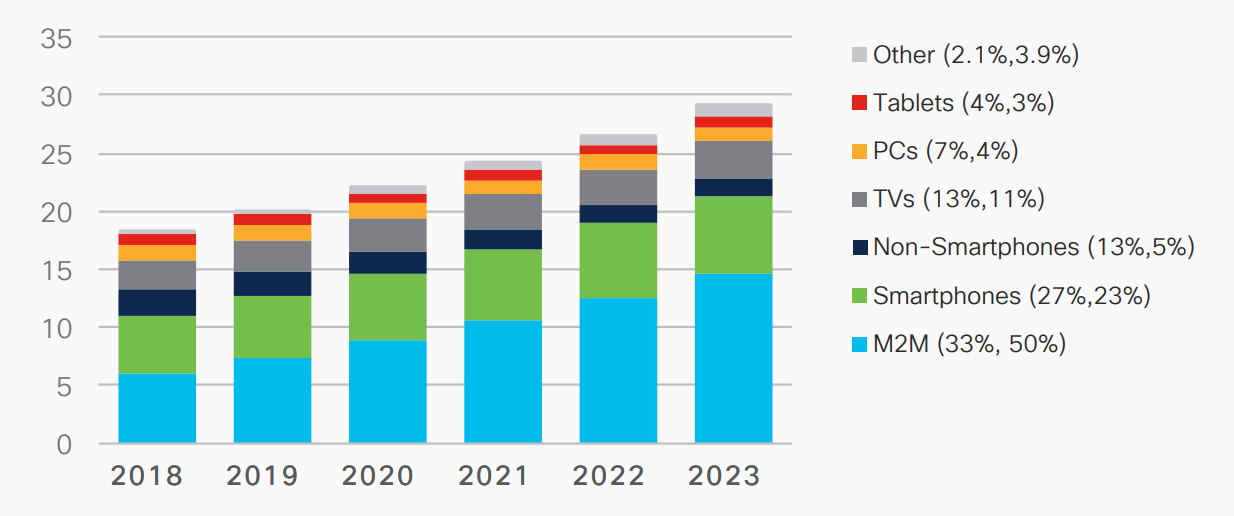
\includegraphics[width=.9\textwidth]{figs/devices growth.PNG}
		\vspace{\baselineskip}
	\caption{Global device and connection growth (billion)~\cite{forecast2019cisco}}
	\label{fig:device_growth}
\end{figure}


In order to address the computational limit of the local mobile devices, Mobile Edge Computing (MEC)~\cite{mec_wp} has recently been introduced as a promising architecture that has the potential to enable cellular networks to offer low latency to mobile applications. MEC equips cellular base stations (i.e., the edge) with computing and storage resources. Such an architecture allows mobile users to work with services deployed in their vicinity and avoid frequent communication with remote cloud services. However, the amount of available resources at the edge is scarce, and thus it is necessary to manage them efficiently to handle the ever-increasing user demands.

Recently, researchers \cite{sfcgeo, visualcomputing, yang2019delay, xu2020nfv} have proposed to apply NFV to MEC to provide more added-values, such as low cost and high efficiency. Network function virtualization (NFV) [4] has emerged as a networking-computing paradigm that enables efficient utilization of computing and networking resources by applying virtualization technologies to offer network services. In this paradigm, network services are implemented as software modules called virtual network functions (VNFs) that can be dynamically deployed, scaled, and chained together to offer a variety of services to users. In particular, the NFV paradigm is well suited to mobile environments where users freely roam at the edge of the network and dynamically change their point of attachment to the network. 
%A critical challenge of using NFV at the edge is the orchestration of service function chains (SFCs). Each SFC is an ordered sequence of VNFs that are chained together to process the user traffic in order to implement a specific network service. SFC orchestration is the problem of placement, routing, and migration of VNFs to minimize the user-perceived service latency with acceptable operational cost
In NFV, service demands are expressed in the form of Service Function Chains (SFCs). An SFC specifies a sequence of VNFs that user traffic has to pass through in order to attain the required service. 
%SFC is a common and flexible model to realize various services with different requirements, and it allows user to separate data processing in different computing units in MEC (\eg\ edge, cloud, local device) and therefore greatly boost processing time and reduce end-to-end latency while providing enhanced management. 
One of the main challenges of implementing SFCs in MEC is the placement of VNFs on the limited resources that are available at the edge, refer to as \textbf{SFC Orchestration}. User mobility further complicates the placement decisions, where due to user mobility, it may be possible to migrate an SFC or part of it closer to the new location of the user to reduce the communication delay, or continue to run the VNFs in their current locations to avoid service migration delays. Therefore, a trade-off between communication delay and migration delay is often considered when placing VNFs at the network edge.
%


\cat{Motiviating Example} An example of SFC orchestration in MEC can be illustrated in visual cloud computing for 3D light detection and ranging (LIDAR) \cite{visualcomputing}, which deal with different data processing stages such as: 1) acquisition; 2) preprocessing; 3) analysis; and 4) postprocessing. The LIDAR pipeline is outlined in figure 1. When scanning and modeling moving objects in 3D space, the processing stages are divided into two categories based on computational needs: (1) small instance processing: Camera metadata data processing, static background registration, and 3D rendering; (2) large instance processing: video camera pose computation, motion segmentation, and dynamic object positioning. In this example, we can consider each processing function as a service function in SFC orchestration, and a good strategy is to place small instance processing functions on the edge nodes that have limited computing resources but shorter access latency and place the large instance processing functions on the cloud that has sufficient capacity but longer access latency.
\begin{figure}
	\centering
	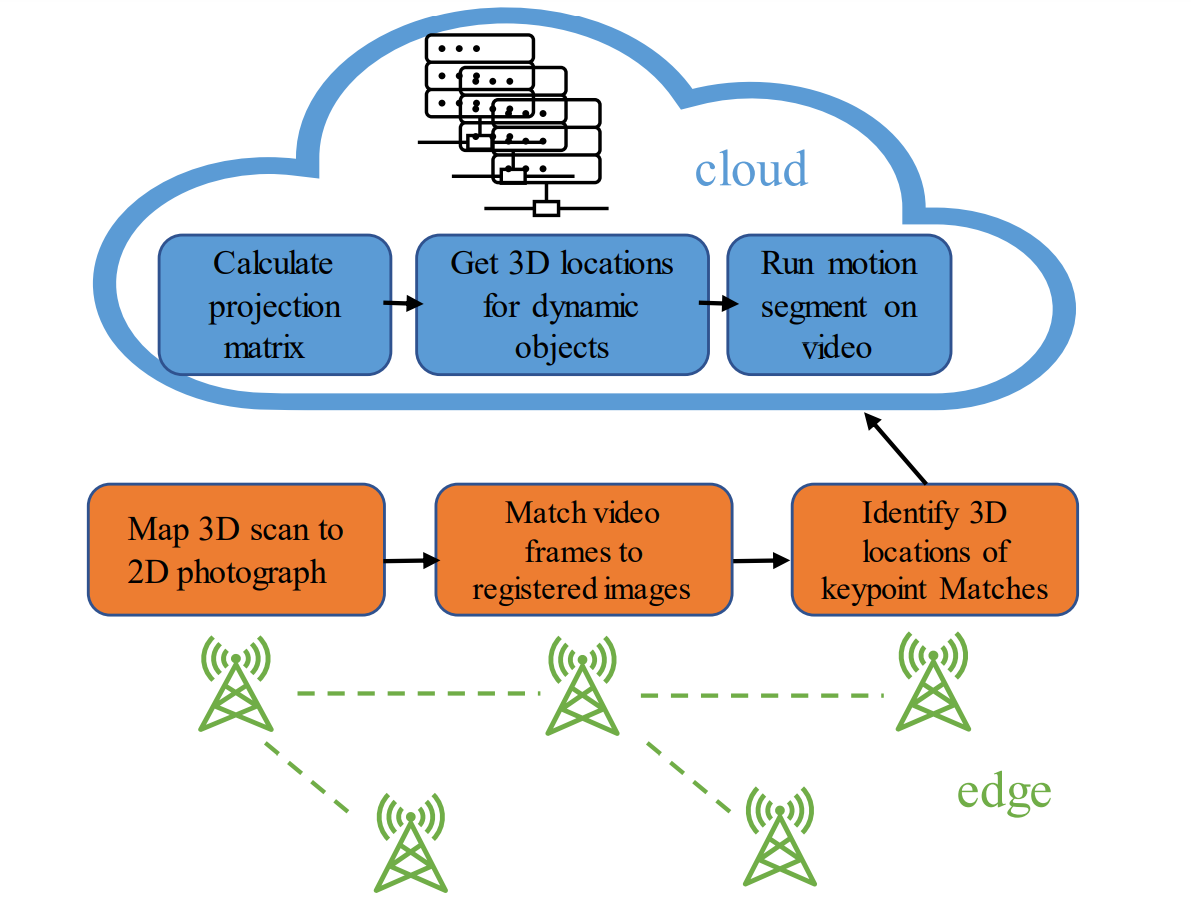
\includegraphics[width=0.9\textwidth]{figs/LIDAR.PNG}
		\vspace{\baselineskip}
	\caption{Example 1: visual cloud computing SFC for 3D light detection and ranging \cite{visualcomputing}}
	\label{fig:lidar}
\end{figure}

Another example of real-time SFC orchestration is shown in figure \ref{fig:geosfc}. This shows a geo-distributed latency sensitive SFC for the computer vision of a real-time object tracking pipeline\cite{sfcgeo}. The pre-processing and Human-Computer Interaction analysis functions are placed on the edge servers while the track function that involves
compute-intensive processing is placed on a cloud server. 
\begin{figure}
	\centering
	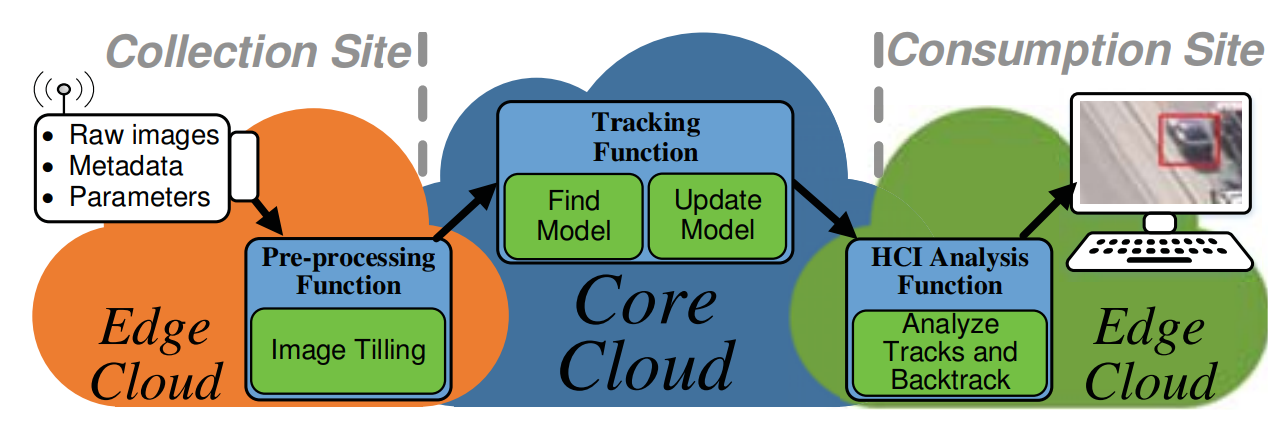
\includegraphics[width=0.8\textwidth]{figs/geosfc.PNG}
		\vspace{\baselineskip}
	\caption{Example 2: geo-distributed latency-sensitive SFC used
		for the real-time object tracking pipeline \cite{sfcgeo}}
	\label{fig:geosfc}
\end{figure}

%The majority of the existing works \cite{dynamicVNFedge, VNF5G, SFCedgecloud, Delay-awareVNFFlexibleResourceAllocation, PosterMEC, VNFmonoedgecore, LatencyAwareMEC} on SFC orchestration in MEC assume that system-wide information such as future service demand, user's mobility and network architecture is known, and one-shot solution is made based on this information, such problem is called \textit{system-managed placement}. However, in real MEC applications, the number of users and the diversity of their services and requirements limit the scalability and customizability of centralized system-managed solutions. \textit{online user-managed placement} is often considered due to user preference and system dynamics, In this model, each user is
%responsible for managing its own SFC with the help of the system that is provided through light-weight feedback.
%Recently, a few works have been proposed to use Reinforcement Learning (RL) based approaches to solve the online user-managed SFC placement~\cite{learningbasedvnf, QPlacement, Environment-AdaptiveRL, OnlineFault-tolerantDRL}. However, most of these works fail to address the SFC placement in a MEC context where features such as user's mobility and service migration are considered.
%Specifically, studies like \cite{MABserviceplacement} show that contextual user-managed algorithms are able to characterize mobile user behavior information and achieve better personalized support, in MEC system where system-level management is difficult due to the complexity of the edge cloud architecture.

The majority of previous research on SFC orchestration has focused on data center settings and does not consider edge resources and user mobility (\eg~\cite{minh_tnsm_20}). Thus, the existing works are not directly applicable to SFC orchestration in MEC. Those works that consider service orchestration in edge-enabled environments belong to one of the two classes: system-managed and user-managed methods. The system-managed methods orchestrate services from a centralized location (\eg~\cite{Spatio_temporal_TWC}). These works have an inherent uncertainty about the users' mobility and face scalability issues as the number of users increases. In contrast,  the user-managed methods enable end-users to manage their services in a distributed fashion based on the system feedback (\eg\ end-to-end delay). Several works use game theory to design user-managed mechanisms~\cite{8247219,8567670}. However, these works do not consider the migration cost and can not adapt to system changes. Recently, a few works have applied reinforcement learning and bandit formulation to provide a higher level of adaptability. In the face of problem complexity, these works have focused on the single VNF orchestration to limit the number of so-called \emph{arms} employed in the bandit formulation (\eg~\cite{MABserviceplacement}). We address this challenge by designing a user-managed SFC orchestration algorithm at the edge that applies reinforcement learning to minimize the user-perceived end-to-end delay while limiting the number of arms required for modeling SFCs by utilizing the theory of combinatorial bandits.


%
Therefore in this work, in order to take users' behavior into consideration while placing SFCs, we stand on the user-side perspective and propose an original contextual online learning approach that can cope with system uncertainty in edge and user-specific context.




\section{Thesis Objective}

In this thesis, we consider the problem of online SFC orchestration by mobile users with no prior knowledge of system side information (\ie, server capacities and link delays) in an edge-enabled environment, with the objective of minimizing the user-perceived end-to-end latency. More specifically, the uses generate a list of VNF demands representing the SFC request and decide which computing nodes they deploy the SFC on, yet they have no knowledge of the infrastructure information, including server capacities and link delays. The SFC orchestration is to decide, from the pool of resources available on the local device (\ie, hand-held equipment), at the edge and in a remote cloud, where to place each VNF of a service in order to minimize end-to-end service delay. In this optimization problem, there are three main difficulties that need to be considered:
\begin{itemize}
	\item \textit{Unknown environment}: The user has no knowledge of system information or future information.
	\item \textit{User's mobility}: User may roam throughout the MEC region during a continuous SFC-related service.
	\item \textit{VNF's migration}: VNF migration may be needed when the user moves too far from their original served region.
\end{itemize}



In our formulation of the problem, we consider the end-to-end service delay incurred due to processing, propagation, transmission, and service migration. We call this problem User-managed Edge-enabled Chain Orchestration Problem (\myproblem) and formulate it as a Mixed-Integer Program (MIP). To solve the problem, we design an algorithm, called \myalgorithm. In \myalgorithm, we employ the contextual combinatorial bandit framework to enable users to efficiently collect information from the environment and compute delay-optimized service placements. The context allows users to incorporate any available information (e.g., about demands) into the resource allocation formulation. We formulate the problem as a combinatorial bandit to focus on the basic user options (i.e., servers and links) during the learning phase of our algorithm, which significantly reduces the solution space of the problem. A naive formulation would force users to consider all possible solutions, whose number grows exponentially in terms of the number of servers and links (e.g., all the different paths in the network). 
Therefore, \myalgorithm\ can efficiently learn about the environment, i.e., fast convergence, without incurring a high processing penalty. For orchestrating services
efficiently, \myalgorithm\ uses a fast dynamic programming-based subroutine to make allocation and migration decisions based on the learned information. Finally, while the majority of exiting works in this area use numerical computations and simulations to evaluate their proposed algorithms, we use Mininet-WiFi to implement our proposed scheme and examine its performance and behavior in an emulated environment with a realistic setting and various mobility models.
%After the learning phase, the actual placement of services is done using a dynamic programming formulation that utilizes the learned information to compute a delay-optimized service placement



\section{Thesis Contribution}
In this section, we summarize the main contribution made by this work, including an overview of our proposed formulation and approach for \myproblem, and the experiments designed for evaluating the proposed approach.

\noindent\textbf{Customized Problem Formulation.}
We formulate the problem of user-managed SFC orchestration at the edge as an integer program by considering user demands, mobility, and end-to-end service delay, in which each formulation characterizes the key features in our work such as network models, delay models, and service models. The main constraints we consider in our formulation is designed to meet the network requirements, such as avoiding co-locating placement, single-path routing, and link bandwidth constraints. The objective of our problem is a weighted sum of four different delays we considered in our model. Specifically, we define multiple scale factors to specify the relative importance of different components of the end-to-end delay.

\noindent\textbf{Problem Transformation via Contextual CMAB.}
Due to the uncertainty of system-wide information and the visibility in the user-side state information, we are able to transform the user-managed SFC orchestration problem into a \textit{contextual combinatorial multi-arm bandit} problem. We formulate the delays in the network as arms that is to be selected and define various parameters to store information such as the unknown system feature and cumulative contextual feature.
The contextual combinatorial formulation allows the user to focus on the primitive options, thus greatly reduces the decision space and incorporate any available information to make better decisions. Furthermore, we adopted the \textit{contextual combinatorial upper confidence bound algorithm} (\ccucb) \cite{C^2MAB} in our decision making to balance exploration and exploitation. Lastly, We present a contextual combinatorial bandit learning algorithm to efficiently learn about the available resources on local equipment, at the edge, and in a remote cloud.

\noindent\textbf{Dynamic programming chain allocation.}
Our \ccmab\ formulation for user-managed SFC orchestration in MEC is an online learning problem that is unlikely to solve optimally due to the environment and time span uncertainty. However, at each learning slot, finding the current optimal SFC placement solution can be solved in a reasonable time with a traditional optimization method.
Therefore, we proposed a dynamic program (DP) based chain allocation method to optimally allocate SFC at each round, which takes the revealed estimates as input and take user-side specific contextual information into consideration. DP finds the optimal solution by starting from placing one single service and successively moving to the next service while taking the previous solutions into account. Our proposed DP-based approach is able to find the per-time-slot optimum in polynomial time.


% \noindent\textbf{Delay measurement framework.}
% A general CMAB framework assumes that, by selecting an arm, a certain estimation or outcome may be revealed. In order to satisfy this assumption, we proposed a time-stamp based delay measurement framework to obtain the delay experienced on a link or node of a SFC path. Moreover, we implement this framework in our Mininet-WiFi emulation.

\noindent\textbf{Simulation and Mininet-wifi emulation experiments.}
We present extensive simulation results to study the behavior of our algorithms under different experiment parameters and problem scales. 
By comparing to the offline optimum, we are able to show that our proposed approach can achieve a close-to-optimum performance.
We also compare the performance of our algorithms against two other greedy-based learning approaches and one offline benchmark to demonstrate the superior performance of the proposed algorithm. 
Furthermore, we simulate a MEC system with user mobility using \textit{mininet-wifi} \cite{mininetwifi} and implement manageable VNFs for each server node.
We then perform a set of experiments in Mininet-WiFi to validate the practical performance of the proposed algorithm.



\section{Thesis Organization.}
The thesis is divided into nine chapters. The content of each chapter is summarized below.

\dog{Chapter 1} discussed the motivation for this study, provides a summary of the current research scope and our research objective, as well as an outline of the main contributions in this work.

\dog{Chapter 2}  provides the necessary background on NFV, MEC, SFC techniques, discusses the online learning approaches as well as the mathematical optimization techniques employed in this study, and gives an overview of the software tools used in experiments.

\dog{Chapter 3} reviews the most relevant literature that focuses on SFC placement problems and classifies them into different categories based on whether they are edge-enabled and user-managed.

\dog{Chapter 4} describes the system model and present the optimization formulation for offline \myproblem.

\dog{Chapter 5} presents the contextual combinatorial bandit formulation for the proposed SFC placement problem and the design of our proposed dynamic programming-based online learning algorithm.

\dog{Chapter 6} presents the design of a time-stamp based delay estimation method that is required in the bandit formulation.

\dog{Chapter 7} presents the extensive simulations results to study the learning behavior of the proposed algorithms and demonstrate their superior performance on scalability compared to the greedy approaches. 

\dog{Chapter 8} presents the Mininet-WiFi experiment results to validate the practical performance of the proposed approach 

\dog{Chapter 9} concludes the thesis with a summary of the works and discussions for future research orientations.









\chapter{\textbf{Backround}}
This chapter presents the background knowledge for understanding our work in this thesis. Particularly, Section \ref{sec:NFV} provides a summary of basic knowledge on NFV architecture. Section \ref{sec: MEC} gives an introduction of the newly emerged MEC technologies. Section \ref{sec: SFC} specifically focus on the SFC architecture and its optimization opportunities. Then, Section \ref{sec:online learning} discusses the online learning techniques and especially the \ccmab algorithm adopted in this work in order to solve the user-managed online SFC orchestration problem. Section \ref{sec:mathematical tools} discusses the mathematical techniques employed in this work to model and solve the offline SFC orchestration on edge. Lastly, Section \ref{sec:software tools} gives an overview of the software tools used for simulation and emulation experiments.


\section{Network Function Virtualization}
\label{sec:NFV}
\subsection{NFV architecture}
Network Function Virtualization (NFV) is a network architecture concept that is first introduced in 2012 by the European Telecommunications Standards Institute (ETSI) \cite{nfv_wp}, in which they propose to softwarize the traditional network appliances that are physically installed (\eg, Deep Packet Inspection (DPI), Firewall, Message Router), and implement these functions in a way that they can be run on a range of industry-standard server, and can be migrated and placed in various locations in the network as required, without the need of installing new physical equipment. Each softwarized implementations of these network appliances are defined as a virtual network function (VNF). These VNFs can be automatically and remotely installed in a shared computing platform and have functionality as their hardware counterparts in principle.
An example of the NFV paradigm is shown in fig \ref{fig:NFVenvironment}, where  specialized middleboxes are replaced with VNFs consolidated on Commodity Off-The-Shelf (COTS) hardware \cite{zhang2020nfv}.
\begin{figure}
	\centering
	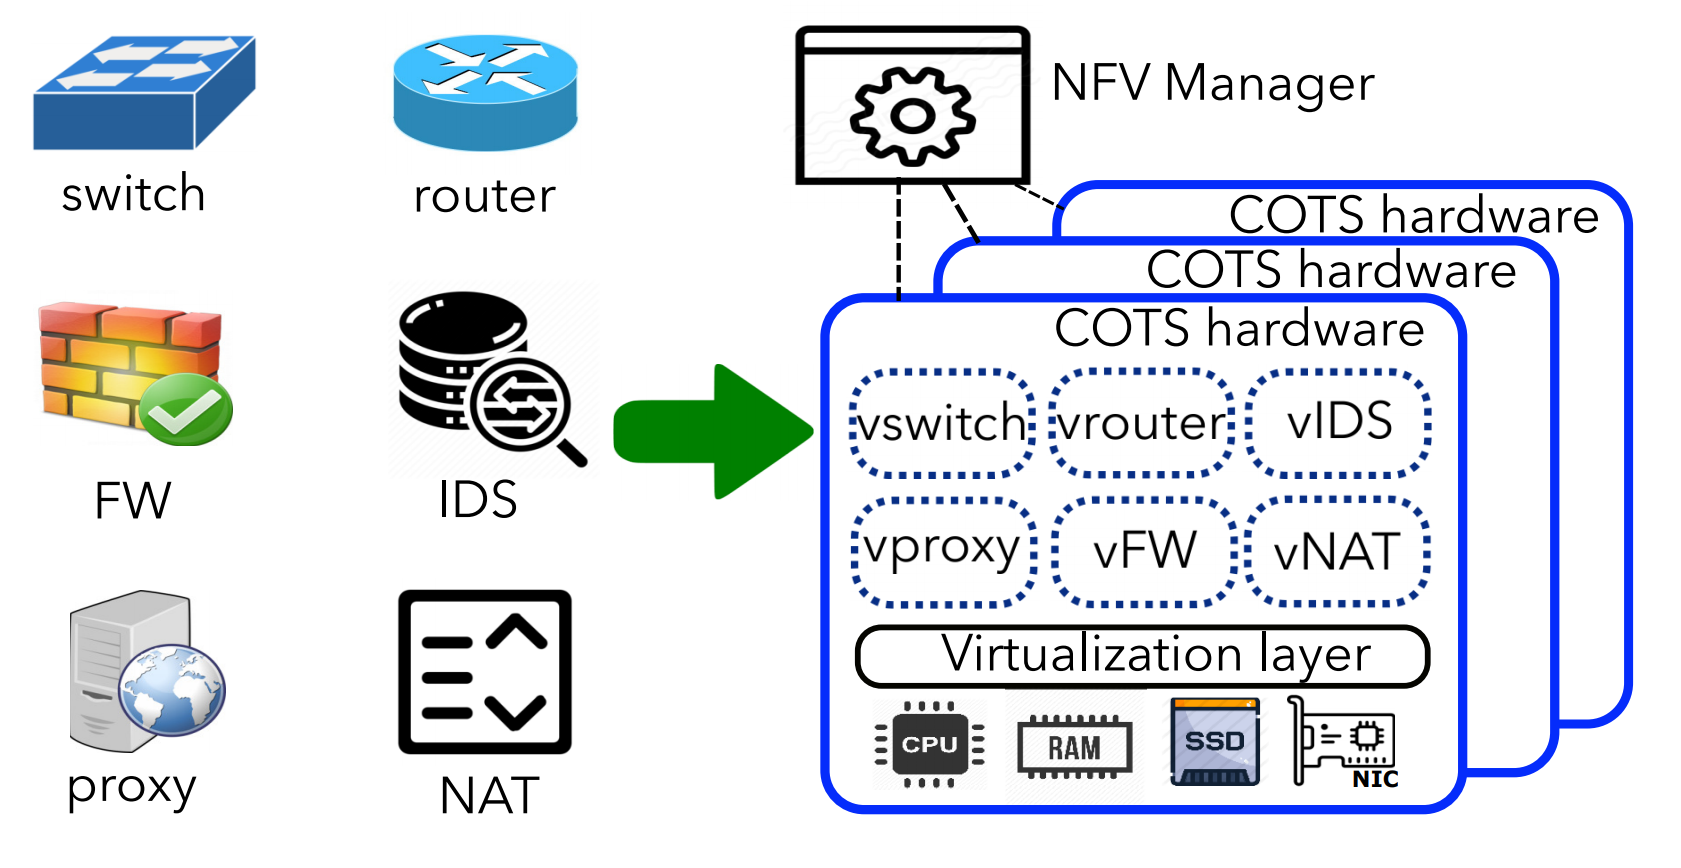
\includegraphics[width=0.9\linewidth]{figs/NFVenvironment.PNG}
		\vspace{\baselineskip}
	\caption{An illustrative example of NFV paradigm \cite{zhang2020nfv}}
	\label{fig:NFVenvironment}
\end{figure}
Virtualising Network Function has potential benefits such as reducing equipment cost, increasing the speed of Time to Market (\ie, the time it takes to implement a network service), and enabling multi-tenancy/multi-version network appliances. Moreover, NFV architecture provides users with enhanced manageability over their personalized applications. 
Compared to traditional network architectures, the advantages of adopting NFV can be summarized according to NFV white paper~\cite{nfv_wp} as follow:
(1) reduced equipment costs, 
(2) improved operating performance and operational efficiency,
(3) optimized network configuration and resource allocation,
(4) flexible network function deployment and dynamic operation, and (5) reduced energy consumption.

\subsection{NFV optimization}
Furthermore, NFV architecture provides various optimization opportunities for researchers such as latency, resource consumption, VNF deployment cost minimization, and utility maximization. In a typical resource allocation problem in an NFV-based network (NFV-RA), there are three stages described below.

1) \textit{VNF chain composition}: VNF chain composition, referred to as Service function Chaining in this work, is the problem of dynamically and strategically composing and deploying SFCs on a set of physical works in an NFV architecture, in order to meet a predefined service requirement. 
%The first challenge is the chaining of the VNFs to implement a requested network service.
%Figure \ref{fig:SFCcomposition} shows an example of two possible chainings of a Virtual Network Functions Request (VNFR), in which the SFC starts from VNF1 and terminates at VNF5, In VNF-FG2,
%the VNF composition is different as the VNF4 precedes VNF3 in the lower branch, which can be another feasible solution.
%\begin{figure}
%	\centering
%	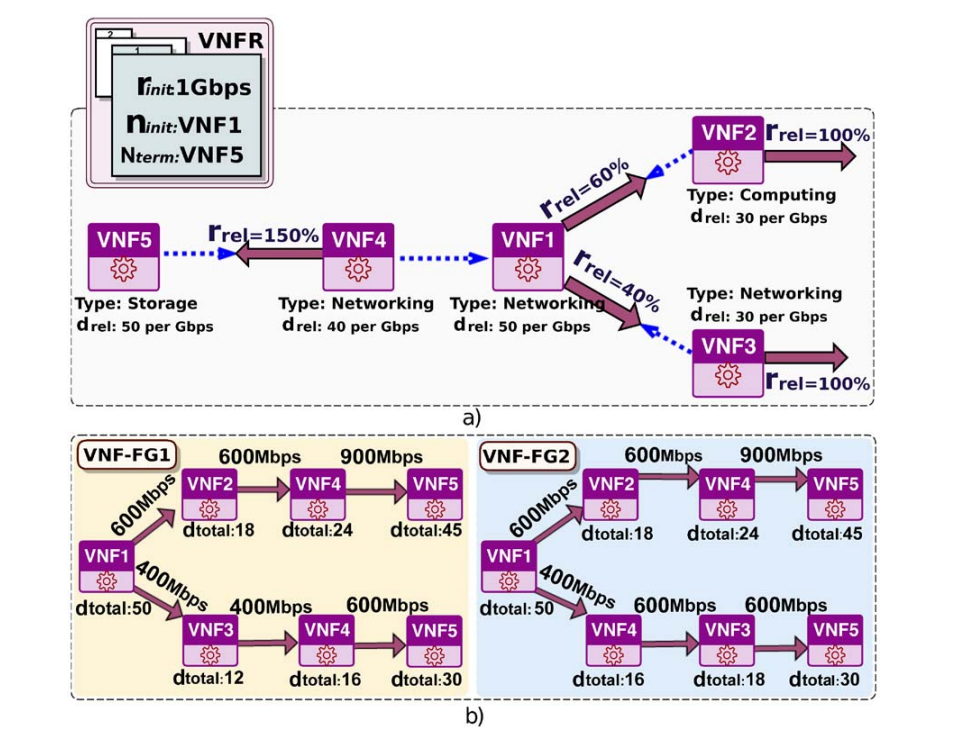
\includegraphics[width=0.9\textwidth]{figs/SFCcomposition.PNG}
%		\vspace{\baselineskip}
%	\caption{VNF Chain composition \cite{herrera2016resource}}
%	\label{fig:SFCcomposition}
%\end{figure}


2) \textit{VNF Chain Embedding}: The second stage is called VNF Chain Embedding, also referred to as SFC placement or orchestration in this work, which aims to find the physical node in the network infrastructure to employ the VNFs that suits the requested network services. Figure \ref{fig:SFC embedding} shows an example of an end-to-end VNF chain (Firewall $\rightarrow$ LoadBalancing $\rightarrow$ Encryption $\rightarrow$ PacketInspection $\rightarrow$ Decryption) embedding.


\begin{figure}
	\centering
	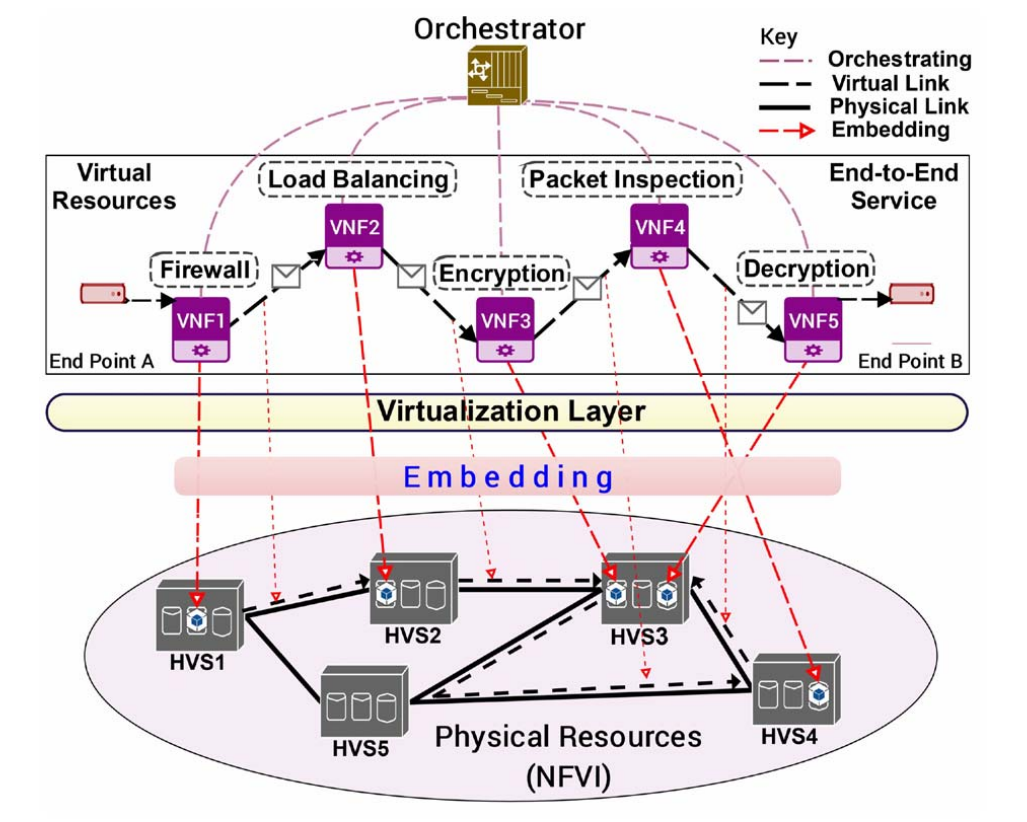
\includegraphics[width=0.9\linewidth]{figs/SFCembedding.PNG}
		\vspace{\baselineskip}
	\caption{VNF Chain Embedding \cite{herrera2016resource}}
	\label{fig:SFC embedding}
\end{figure}

3) \textit{VNF Chain Scheduling}: The final stage is to schedule the VNFs on the chain properly. Specifically, this stage seeks to minimize the total execution time of the requested network services by scheduling the execution of each VNF, for example, execute some VNFs simultaneously or execute each VNF in order of the chain. 
%Figure \ref{fig: VNF Chain Scheduling} showing an example of how the same VNF chain can be scheduled in three different ways.
%\begin{figure}
%	\centering
%	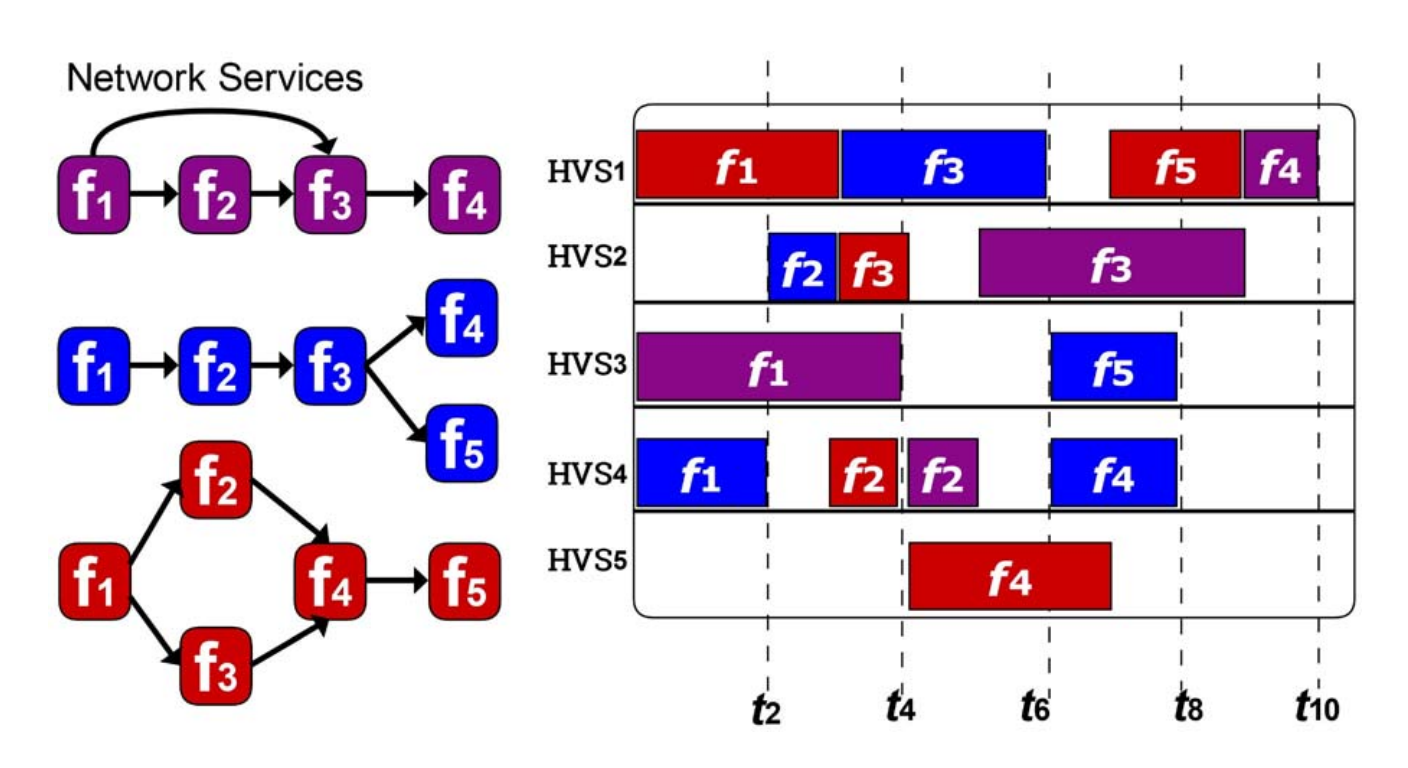
\includegraphics[width=0.9\linewidth]{figs/VNFSchedule.PNG}
%		\vspace{\baselineskip}
%	\caption{VNF Chain Scheduling \cite{herrera2016resource}}
%	\label{fig: VNF Chain Scheduling}
%\end{figure}


In this work, our focus is mainly on the second stage of an NFV-RA problem, that is, the placement/embedding/orchestration of the VNF chain to physical, we refer to it as \textbf{SFC orchestration} in this thesis. In section \ref{sec: SFC} we further discuss the standard SFC architecture,  mathematical and algorithmic approaches for SFC orchestration.






%The work in this thesis concerns the minimization of end-to-end delay while taking resource consumption into consideration. 

\section{Mobile Edge Computing}
\label{sec: MEC}
\subsection{MEC architecture}
Mobile Edge Computing (MEC) was first standardized by European Telecommunications Standards Institute (ETSI) and Industry Specification Group (ISG), it is introduced as an integration of edge computing (also known as fog computing) and mobile computing, which empowers Mobile Cloud Computing (MCC) by distributing cloud resources (\eg storage and processing capacity) to the edge servers inside the range of radio access network (RAN). 
An illustration of a MEC system is shown in fig \ref{fig:MECachitecture}, which consists of two major components: mobile devices (e.g. end-users, clients, and service subscribers) and MEC servers. MEC server is usually
a small data center deployed by cloud and telecom operators that can be placed close to the end-user and co-located with the wireless APs. The edge servers are connected to the data centers through a gateway via a backbone internet, while mobile devices are connected to the edge servers via a well-established wireless link implemented using advanced wireless communications and network technologies \cite{MECsurvey}.
%
In section \ref{section: system model} we present our system model formulation for MEC that consist of one cloud center and multiple edge servers.
%
\begin{figure}
	\centering
	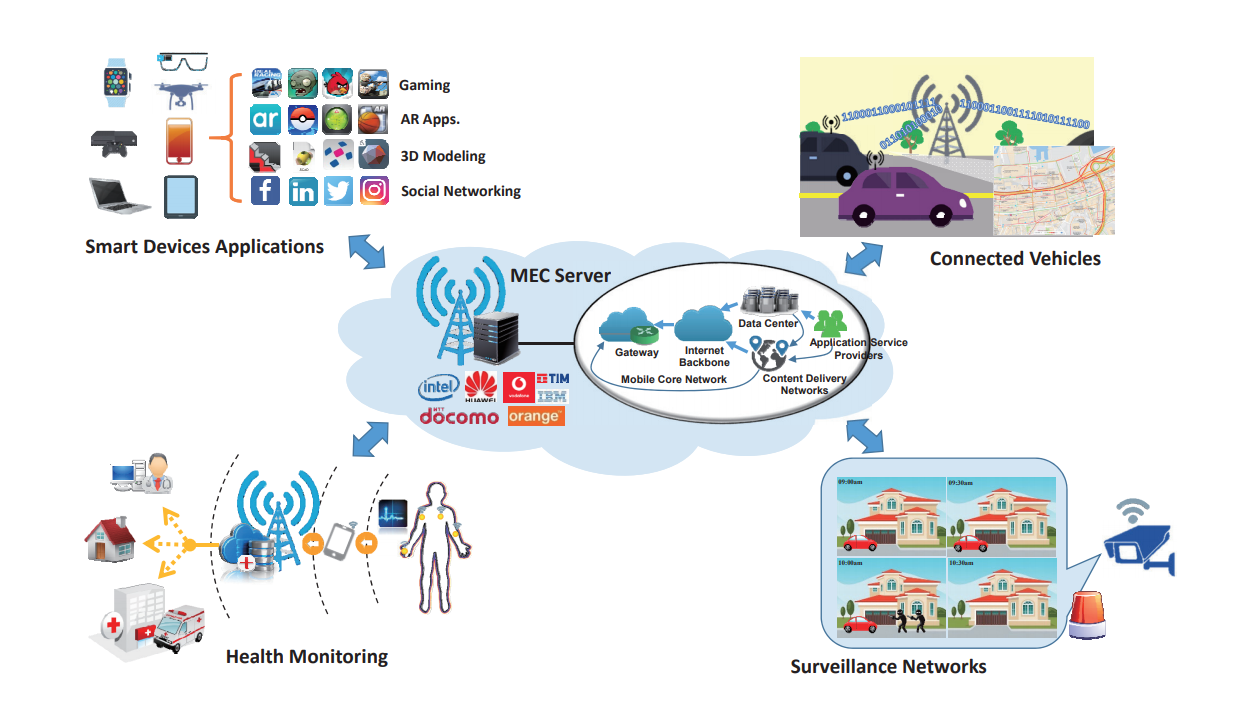
\includegraphics[width=0.9\linewidth]{figs/MEC architecture.PNG}
		\vspace{\baselineskip}
	\caption{Architecture of the MEC system \cite{MECsurvey}}
	\label{fig:MECachitecture}
\end{figure}

Numerous works in different fields have been discussed in the literature that can be exemplified as a application scenario for MEC, including but not limited to: Health care \cite{apphealthcare1}, Video Analytics\cite{appvideoanalytics1}, Mobile Big Data Analytics \cite{appmobilebigdata1}, Connected Vehicles \cite{appconnectedvehicles1}, Smart Grid\cite{appsmartgrid1}, Wireless Sensor and Actuator Networks \cite{appwsn1}, Smart building Control, SDNs \cite{appsdn1}, Ocean Monitoring \cite{appoceanmonotoring1}. According to the white paper published by ETSI \cite{MECwhitepaper}, a brief summary of the key features of MEC is characterized below.

\cat{On-premises} MEC can run isolated from the rest of the network while having access to local resources. This plays an essential role in Machine-to-Machine (M2M) scenarios such as security or safety systems that require high-level resilience.

\cat{Proximity} Being close proximity to resources, MEC has an advantage in capturing and analyzing big data. It also provides direct access to devices, which can benefit compute-hungry applications such as augmented reality (AR) and video analytics.

\cat{Lower Latency} Edge server is usually deployed at the nearest location of the mobile user, which considerably reduces user-perceived latency to their devices. This can greatly boost user experience and reduce the congestion of other parts of the network.

\cat{Location awareness}  MEC devices can utilize low-level signaling information to determine the location of other connected devices under different types of the wireless network, which provide mobile users with location-based services and analytics.

\cat{Network context awareness} RAN Real-time network information such as the congestion of the radio cell and network bandwidth can be estimated by applications that adopt MEC in their implementation. This offers context awareness that can help to improve the mobile user's experience.

In summary, MEC provides the end-user with swift and powerful computing, energy efficiency, storage capacity, mobility, location, and context awareness support. 
%

\subsection{MEC research topics}
MEC has provided numerous research topics in computer science, and we summarize the main topics that have been studied in this area and discuss where our work stands.

\cat{Computational Offloading}
The most discussed research topic in the MEC area is computation offloading, which is the process of migrating computing tasks to external resources such as clouds, grids, or clusters \cite{ma2013mobile}.
This increases the computing ability of mobile devices by running computing-intensive and resource-demanding applications (e.g. 3-D gaming and video encoding) on edge cloud. 
For example, offloading web application execution on the edge servers that is within the RAN can accelerate web browsing \cite{takahashi2015analysis}.

Using well-designed algorithms and approaches, the computational offloading process can also be optimized in a radio access environment, which can reduce signal interference and energy consumption \cite{chen2015efficient, sardellitti2015joint}. 



\cat{Low Latency}
MEC can greatly improve users' experience by lowering the latency of their requested applications and services. 
For example, latency can be effectively reduced by intelligently scheduling memory replication events in the edge cloud while resolving conflicts for wireless resources\cite{abdelwahab2015replisom}.
%
Integrated with 5G technologies, MEC can provide real-time context-aware support for applications such as live remote robotic telesurgery and road accident\cite{nunna2015enabling}, which require context-information (e.g. geographical information). MEC allows ultralow latency for these applications by satisfying the context demands.
%
MEC can also support vehicular delay-tolerant network by utilizing smart grid devices that communicate with the MEC environment. It addresses the communication complications caused by the high mobility of vehicles by interacting with mobile smart devices that monitor the data sets\cite{kumar2016vehicular}.

\cat{Storage support}
MEC also provides users with additional storage support when their local device storage is limited. MEC storage capabilities can be further enhanced by integrating with virtualization techniques such as software-defined network, software-defined compute, and software-defined storage\cite{jararweh2016sdmec}, which enable the support for storage/computing-intensive applications such as traffic monitoring and mobile gaming.

\cat{Energy Efficiency}
By running computational tasks on edge cloud architecture, MEC can reduce the energy consumption of users' local devices. 

For example, mobile devices can share the energy and computational resources on edge by adequately estimating the network status, which ensures the computation time is synchronized \cite{gao2014opportunistic}. 
%
MEC can significantly prolong the battery lifetime of user devices by offloading computing-intensive tasks like video encoding to the edge servers that employ advanced encoding services\cite{beck2015me}. Instead of migrating computing-intensive to the edge, MEC architecture can also coordinate resources between resource-rich mobiles devices and resource-constraint mobile devices in order to escalate the power management of these devices.

In this work, our focus is on computational offloading and latency reduction in MEC architecture. In particular, we consider the optimization of the end-to-end latency to run SFCs in MEC, for which we design an online SFC orchestration algorithm and offload SFC tasks accordingly.







\section{Service Function Chain}
\label{sec: SFC}
Service Function Chain is defined as a sequence of multiple VNFs that user's traffic has to traverse through to realize their required services. This section provides some background knowledge of SFC, including SFC architecture, SFC request model,  SFC Resource allocation problems, and optimization approaches.
\subsection{SFC architecture}
A typical SDN-based SFC architecture consists of the SFC control plane and  SFC data plane, as defined by the IETF SFC and ONF working groups. Fig \ref{fig:SFCachitecture} shows an illustration of a standard SFC architecture that is explained as follows:

\cat{SFC control plane} The control plane is responsible for the management of SFC, such as the management of each service function instance (SFI), the mapping of SFC to a specific service function path (SFP), the administration of forwarding rules, and the adjusting of SFP with regards to the link status.

\cat{SFC data plane} SFC data plane consist of: SFC classifier, Service function forwarding (SFF), Service function (SF) and SFC proxy. the SFC classifier differentiates the incoming traffic into flows and tags each flow with an SFP header. An SF executes a particular set of actions on the incoming packets (e.g deep packet inspection or firewall functions). An SFC proxy de-capsulate the packets when the majority of SFs do not recognize the SFC packet headers.
\begin{figure}
	\centering
	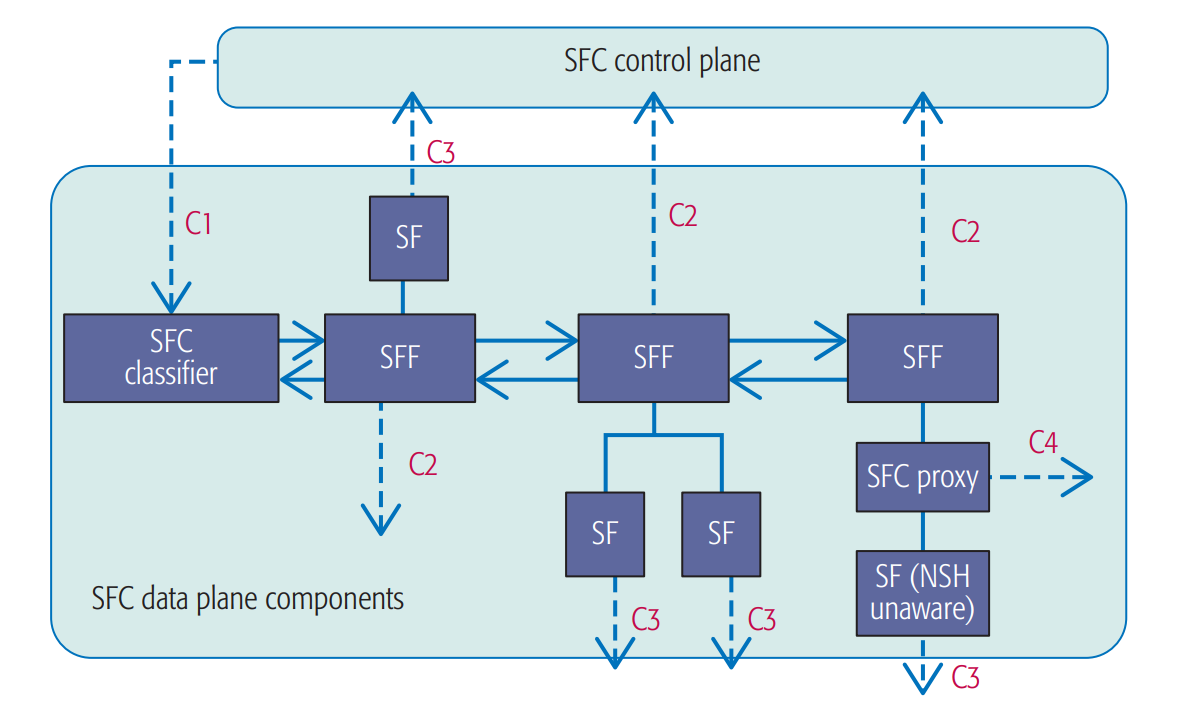
\includegraphics[width=0.9\linewidth]{figs/SFCarchitecture.PNG}
		\vspace{\baselineskip}
	\caption{A typical SFC architecture \cite{medhat2016service}}
	\label{fig:SFCachitecture}
\end{figure}

\subsection{SFC request model}
In order to realize a particular service, the user's traffic flow must be directed through an ordered sequence of VNF instances. For example, an SFC of NAT, FW, and IDS, as depicted in fig \ref{fig:SFCrequestmodel}. The set of enabled services represents the operators'
services, which is built according to the service agreements between
operators and end-users with regards to network policies \cite{xie2016service}

An SFC request is a source-to-destination path that contains an ordered list of service functions, and the users may have various bandwidth and computational demands for each service function. We model our SFC demand in section \ref{sec:SFCrequest}, in which we define $\lambda$ as the user-generated traffic rate and add customized scale factor $\alpha_{s_i}$ to it with respect to each type of service $s_i$.

\begin{figure}
	\centering
	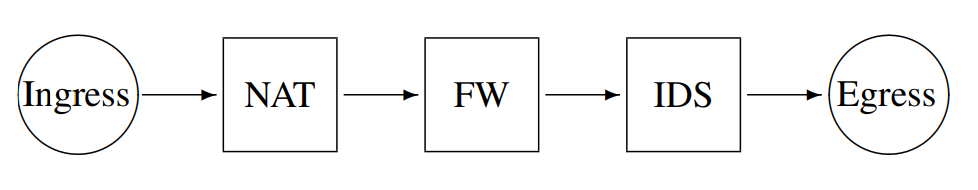
\includegraphics[width=0.9\linewidth]{figs/SFCrequestmodel.PNG}
		\vspace{\baselineskip}
	\caption{Service Request Model \cite{xie2016service}}
	\label{fig:SFCrequestmodel}
\end{figure}

\subsection{SFC orchestration problem}

\cat{Delay Aware} In a delay-aware SFC orchestration problem, a physical network and a set of service requests are given, as well as the number of needed VNF types and demand specifications. The goal is to minimize the total end-to-end delay. Therefore delay-aware SFC orchestration problem has two steps:

\begin{enumerate}
	\item Calculate the latency on each link and node with regards to the service demand and capacity.
	\item Place SFCs to physical nodes and links such the total end-to-end delay is minimized.
\end{enumerate}

\noindent In addition, a virtual link on SFC may be placed on several physical links.

\cat{Cost Aware} The objective of the cost-aware SFC orchestration problem is to minimize the deployment cost when placing SFCs to physical nodes and links, which is often expressed as the resource and bandwidth consumption.








\subsection{SFC orchestration optimization approaches}
To orchestrate a SFC via an NFV architecture, the user needs to choose a set of computing platforms to install each VNF on a SFC and decide the SFC's routing order while considering various constraints such as fluctuated SFC demands and quality of service (QoS). The problem of SFC orchestration is one of the main challenges in NFV. Therefore many works have taken aims at addressing it, and many optimization approaches have been investigated. They can be summarized as below.

\cat{Exact and approximation solutions} SFC orchestration problem can be typically formulated into: Integer Linear Programming (ILP) or Mixed Integer Linear Programming (MILP). We can use traditional exact approaches to solve ILP, \eg, \textit{dynamic programming, branch and bound, cutting plane methods}
The work in this thesis uses DP to solve per-time-slot SFC orchestration in a guaranteed time. \textit{Approximation solutions} give a trade-off between optimal solution and algorithm complexity, which achieves a near-optimal but polynomial-time performance.

\cat{Heuristic solutions}
In practice, SFC orchestration is required to be low latency or real-time. Thus fast heuristics-solution is often preferred due to the hardness of the SFC orchestration problem. \eg, \textit{simulated annealing, tabu search, genetic algorithm, ant colony, best-fit decreasing}. 


\section{Learning algorithm}
In this section, we discuss the learning algorithms we applied in this work.
\label{sec:online learning}
\subsection{Online learning}
Online learning is the process of taking actions given knowledge of rewards of the previous actions and possibly available information. It takes place in continuous rounds. On each round, the learner is presented with a set of actions and is required to take one of them. The goal of online learning is to maximize the accuracy of the learner's predictions so that correct decisions can be made, which is in contrast to a traditional offline learning method that is to learn a model from the entire training data set at once \cite{hoi2018online}. 
Therefore, online learning can instantly learn from newly arrived data and are easier to implement than offline learning. In this work, user-managed SFC orchestration can be modeled as an online learning process due to the sequentialness of the user requests.

Online binary learning can be exemplified as a simple online learning, where the reward/outcome of each action is binary: yes or no.  Algorithm \ref{alg:online binary learning} summarizes a brief procedure of online binary learning, where $\nb{x}_t$ denotes the sequential instance and $y_t$ denotes the binary reward label of each instance. At each round, the learning use vector $\nb{w}_t$ as a prediction model to calculate the predicted reward label : $\hat{y}_t = \textnormal{sign}( \textbf{w}_t^\top \textbf{x}_t)$. Then the learner receives the true reward label $y_t$ after taking the predicted action, and calculate the suffered loss: $l_t(\textbf{w}_t) = \textnormal{max}(0,1-y_t\textbf{w}_t)^\top \textbf{x}_t)$. Lastly, the learner strategically update the prediction model based on the loss and true labels received. 
\begin{algorithm}
	\caption{Online Binary Learning}
	\label{alg:online binary learning}
	Initialize the prediction function as \textbf{w_1};\\
	\For{$t=1,2,...,T$}{
		\textnormal{Receive instance: $\nb{x}_t \in \mathbb {R}^d;$}\\
		\textnormal{Predict $\hat{y}_t = \textnormal{sign}( \textbf{w}_t^\top \textbf{x}_t);$} \\
		\textnormal{Receive the true reward label: $y_t \in \{ -1, +1\};$}\\
		\textnormal{Suffer loss: $l_t(\textbf{w}_t) = \textnormal{max}(0,1-y_t\textbf{w}_t)^\top \textbf{x}_t);$}\\
		\textnormal{Update the prediction model} $\textbf{w}_t$ to $\textbf{w}_{t+1};$
	}
	\textnormal{Calculate regret:} $R_T = \sum^T_{t=1} l_t({\bf w_t}) - \min _{\bf w} \sum_{t=1}^T l_t({\bf w});$
\end{algorithm}





\subsection{Bandit online learning}
As an import branch of online learning, Bandit online learning, a.k.a. Multi-Armed Bandit (MAB) problem, has been studied extensively in the online learning community.
MAB is normally formulated as a sequential decision-making problem where the decision-maker is presented with $m$ arms to select from at each of $n$ rounds, where $T$ is often unknown at the beginning and decisions are made based only on the feedback from the environment. The distribution of reward on each arm is unknown, and the goal of the problem is to maximize the total reward or minimize the total loss over the course of $n$ rounds, with $a_t$ denoting the action of each round, $r_t(a_t)$ and $l_t(a_t)$ denoting the reward and loss of that action respectively. We can formally define the "regret" as the difference of cumulative loss between the optimal arms and player selected arms:
\begin{equation}
	R_T = \sum\limits_{t=1}^T l_t(a_t) - \min\limits_{i\in[m]} \sum\limits_{t=1}^T l_t(i)
\end{equation}
One of the major challenges of MAB is how to trade-off between \textit{exploitation} and \textit{exploration}, where \textit{exploitation} of past actions ensure high payoffs based on the past knowledge and \textit{exploration} of new actions gives possibly higher payoffs in the future, which is also one of the major concerns in this work.


\cat{$\epsilon$-Greedy Multi-Arm Bandit}
The first simplest MAB based algorithm is $\epsilon$-Greedy MAB introduced in \cite{sutton1998introduction}, in which the player plays the arm that currently has the highest average reward with probability $1-\epsilon$ and plays a random arm with probability $\epsilon$, where $\epsilon$ is a constant value in (0, 1). $\epsilon$-Greedy Multi-Arm Bandit algorithm is summarized in algorithm \ref{alg:greedymab}, where $N_{i_t}(t)$ denote the number of times arm $i$ has been selected by the player until $t$ rounds and $\mu_{i_t}$ denotes the mean of the rewards received on arm $i$. 

In this work, $\epsilon$-Greedy Multi-Arm Bandit algorithm is used as a performance comparison in experiments presented in chapter \ref{chapter:simulation} and \ref{chapter: Mininet-wifi Experiments}. 

\begin{algorithm}
	\caption{$\epsilon$-greedy MAB}
	\label{alg:greedymab}
	\textbf{INPUT:} parameter $\epsilon > 0$\\
	\textbf{INIT:} empirical means $\mu_i = 0, \forall i \in [m]$\\
	\For{$t=1, 2, ..., T$}{
		with probability 1-$\epsilon$ play the current best arm $i_t = \textnormal{argmin}_{i\in[m]}\mu_i$\\
		with probability $\epsilon$ play a random arm\\
		receive $l_t(i_t)$ and $r_t(i_t)$\\
		update the empirical means $\mu_{i_t} = (\mu_{i_t}*N_{i_t}(t) + r_t(i_t))/(N_{i_t} + 1)$\\
	}
	
	
\end{algorithm}







\cat{Contextual Combinatorial Multi-Arm Bandit}
In the framework of a Combinatorial multi-armed bandit (CMAB), the decision-maker needs to select a set of arms(referred to as a super arm) and play it,  after a super arm is played and the reward of each arm in the super arm and other triggered arms are revealed at each round. When each arm can be characterized by a feature vector that the decision-maker is able to observe, the problem is known as Contextual Combinatorial Multi-arm bandit (\ccmab) problem, which is often used to adapt to user feedback and diverse interest.
Our work is inspired by the contextual combinatorial upper confidence bound algorithm (\ccucb) presented in \cite{ccmab}, which is a general algorithms for addressing \ccmab problems. \ccucb\ characterize the user-observed context using a set of
feature vectors $\textbf{X}_t = \{\textbf{x}_t(i), ..., \textbf{x}_t(m)\}$ corresponding to $m$ arms at each round $t$ and use vector $\theta_*$ to characterize the system feature, which is unknown to user. 
\ccucb\ then define the reward function on each arm to be:
\begin{equation}
	\label{eqn:computesore}
	r_t(i) = \theta_*^T\textbf{x}_t(i) + \epsilon_t(i),
\end{equation}
where, $\epsilon_t(i)$ is a zero-mean random variable that represent the noise in the system. The goal of \ccucb\ is to maximize the expected cumulative reward $\E [\sum_{t\in n}R_t(S_t)]$ over n rounds, where $R_t(S_t)$ represent the sum reward received for all the arms on the selected super arm $S_t$ at round $t$.
The algorithm use the feature vectors and previously observed rewards to maintain a confidence set for true parameter $\theta_*$, which is then used to compute an reward upper confidence bound for each arm:
$ \hat{\textbf{r}}_t = {\hat{r}_t(1), ..., \hat{r}_t(m)} $
according to equation \ref{eqn:computesore}. $\hat{\textbf{r}}_t$ and $\textbf{X}_t$ is taken as a input to a computation oracle that computes the optimal or near-optimal super arm $S_t$. The algorithm plays the returned super arm and update the confidence sets using the observed rewards on the super arm.
The pseudocode of \ccucb\ is summarized in algorithm \ref{alg:ccucb}, 
where $\alpha_t$ is an approximation ratio that shows the proximity of the current solution to the optimal solution, $\textbf{V}_t$ and $\textbf{b}_t$ are two auxiliary vectors used to update the system paramter $\theta_t$.

In this work, chapter~\ref{chapter: Proposed Method} presents our proposed algorithm that adopts the \ccucb\ framework, which uses an optimal oracle that is based on dynamic programming (e.g, $\alpha_t = 1$)

\begin{algorithm}
	\caption{\ccucb}
	\label{alg:ccucb}
	\textbf{Input:} \alpha_1, ..., \alpha_n\\
	Initialize \textbf{V}_0 \leftarrow \textbf{I}_{d\times d}, \textbf{b}_0 \leftarrow \textbf{0}_d \\
	\For{t \leftarrow 1, ..., n}
	{
		$\hat{\theta}_t$ \leftarrow \nb{V}^{-1}_{t-1}\nb{b}_{t-1}\\
		\For{i \leftarrow 1, ..., m}{
			$\bar{r}_t(i)$ \leftarrow \hat{\theta}_t^T \textnormal{\bf x}_t(i)\\
			$\hat{r}_t(i)$ \leftarrow \bar{r}_t(i) + $\alpha_t\sqrt{\textnormal{\bf x}_t(i)^T \nb{V}_t^{-1}\textnormal{\bf x}_t(i)}$
		}
		\textbf{S}_t \leftarrow \mc{O}({\hat{\textbf{r}_t}}, \textnormal{\bf X}_t)\\
		\textnormal{Play super arm }\textbf{S}_t \textnormal { and observe} \{r_t(i)\}_{i\in S_t}\\
		\nb{V}_t \leftarrow $\nb{V}_{t-1}$ + \sum_{i\in S_t}\nb{x}_t(i)\nb{x}_t(i)^T\\
		\nb{b}_t \leftarrow \nb{b}_{t-1} + \sum_{i\in S_t} r_t(i)\nb{x}_t(i)\\
	}
\end{algorithm}



\section{Mathematical Tools}
\label{sec:mathematical tools}
In this section, we present the two mathematical tools we used for the optimizations considered in this work.
\subsection{Integer Linear problem}
Integer Linear problem is a type of constrained optimization, which consists of an objective function and a set of constraints. In ILP, all the variables in the objective function are restricted to be integers while all the functions and constraints are linear. In this work, we formulate \myproblem\ as a specific form of ILP that is Binary integer linear problem (BILP), in which all of the variables are binary, that is, they can only take on the value of 0 or 1. This  is often used to represent a selection or rejection of an option, \eg\ a yes/no answer, a turning on/off of a switch, and in our work, a decision of whether or not to select a certain node and link.
Formulation \ref{ILP} illustrates an example of a standard constrained binary integer linear problem. In this program, $x_i$ are the \textit{variables} while $c_i$ and $a_{i,j}$ are the \textit{constant coefficient},  the expression \ref{ILP:objective} describes the objective of the BILP as a linear function of variable $x_i$, expression \ref{ILP:const1} and \ref{ILP:const2} are the inequality and equality constraints that $x_i$ is subjected to respectively , while expression \ref{ILP:const3} restrict $x_i$ to be variables only. An standard form also restricts that the variables are ordered according to the objective function coefficients, which is expressed in constraint \ref{ILP:const4}.
\begin{problemenv}
	\caption{A Standard Binary Integer Linear Program}
	\begin{subequations}
		\label{ILP}
		\begin{align}
			\label{ILP:objective}
			\textbf{ Minimize Z =}  & \sum_{i=1}^nc_ix_i\\
			\label{ILP:const1}
			\textbf{Subject to:}  &\sum_{j=1}^n a_{ij}x_j \leq b_i, \quad\forall i \in {1, 2,    ..., h}\\
			\label{ILP:const2}
			&\sum_{j=1}a_{ij}x_j = b_i, \quad\forall i \in {h+1, h+2, ..., m} \\
			\label{ILP:const3}
			& x_i =  0\ \text{or}\ 1,\quad \forall \in {1, 2, ..., n}\\
			\label{ILP:const4}
			& 0\leq c_1\leq c_2 \leq ...\leq c_n 
		\end{align}
	\end{subequations}
\end{problemenv}

The formulation above may seem restrictive, but it is easy to convert many problems to this form. For example, we can handle the negative objective function by simply replacing $x_i$ with $1-x_i$. Negative constraints can also be handled by converting $\leq$ form to $\geq$ form, and reordering the variables is easy.

\cat{Linearization}
A common linearization of BILP is to linearize a product of multiple binary variables, which can be done by a general method showed in formulation \ref{BILP:linearization}, 
where a product of $n$ binary varibles $x_i$ can be represented by a new binary variable $z$ and additional constraints. The linearization concerned in this work is a product of two binary variables, more specifically, we linearize the migration delay part of the objective using this method as expressed in equation \ref{eqn:objlinearization}.
\begin{problemenv}
	\caption{BIP Product Linearization}
	\label{BILP:linearization}
	\begin{equation}
		\begin{align}
			&z = \prod_{i=1}^n x_i\\
			&z \leq x_i\\
			&z \geq x_i-(n-1)
		\end{align}
	\end{equation}
\end{problemenv}


\subsection{Dynamic program}
A recursive algorithm can be designed to solve the problem more efficiently by taking advantage of the similarities in the substructures of a
problem,\cite{IntroductiontoAlgorithm}.
This type of algorithm first divides the problem into many subproblems recursively, each of which has the same structure. The algorithm then repeatedly calls itself to solve each subproblem. Because the problem is divided recursively, there are many instances where subproblems in different branches of the recursion tree are exactly identical to one another.
Rather than separately solving all subproblems,
which wastes computing resources and time, Dynamic Programming proposes to store the results of the subproblems and reuse them when necessary \cite{IntroductiontoAlgorithm}. By apply such a simple technique,
the number of recursive steps needs to solve the problem can be reduced from exponential to polynomial. DP is an optimization approach that has been widely used in common problems such as Min/Max
Knapsack, Shortest Path, and Shortest Common/Uncommon Subsequence, etc. With respect to this work, Dynamic Programming is applied to solve the recurrence equation \ref{DP:recurrence relation}, which is used to find the optimal per-time-slot solution of SFC orchestration.
The idea of the DP-based SFC orchestration is first to compute the optimal solutions for small subproblems (mapping a virtual service function and its associated virtual) and store those values, which is then used to solve larger subproblems until the overall problem (a whole SFC) is solved.
A general DP framework for SFC orchestration is presented in algorithm \ref{alg:DP_SFC}, in which each VNF is assigned with a matrix $D_i$ that stores the cost of sub-optimal SFC orchestrations through iterations and eventually the complete SFC orchestration. Specifically, diagonal elements ($D(j,j)$) of the matrix store node-related cost and none-diagonal elements ($D(k,j)$) store link-related cost. 

\begin{algorithm}
	\caption{A general DP algorithm for SFC orchestration}
	\label{alg:DP_SFC}
	\textbf{Input:} SFC (\textit{s} services), \textit{n} computing nodes\\
	\textbf{Output:} hostsList: substrate nodes hosting the SFC\\
	Initialize $D \leftarrow \textbf{I}_{s\times n\times n}, C \leftarrow \textbf{I}_{s\times n}, H \leftarrow \textbf{I}_{n\times s}$\\ 
	\For{$i = s-1; i \geq 0; i--$}{
		\textnormal{Associate a Matrix $D_i$ to each $vnf_i$}\\
		D_i(j,j) = cost(vnf_i, j)\\
		D_i(j,k) = cost((vnf_i, vnf_{i+1}), (j, k))\\
		\textnormal{Associate a hostList $H_j$ for each $D_i(j,j)$ to store the computed chain mapping }\\
		\For{$j = 1 \rightarrow n$}{
			$ minCost = \infty$ \\
			\For{$k = 1\rightarrow n$}{
				\If{$minCost \geq C$}{
					C(vnf_i, j) = D_i(j,j) + D_{i+1}(k,k) + D_{i+1}(j,k)\\
					minCost = C(vnf_i, j)\\
					host_{i+1} = k\\
				}
			}
			
			D_i(j,j) = minCost\\
			\textnormal{Add $host_{i+1}$ to $H_j$}\\
		}
	}
	\textnormal{Extract the minimum SFC cost from $D_1$by computing the minimum diagonal value }\\
	C(SFC) = \textnormal{min}(D_1(j,j))\ \forall\  j \in [1, n]\\
	Extract the optimal SFC mapping from $H$\\
	
	
\end{algorithm}




\section{Software Tools}
\label{sec:software tools}
In the simulation experiments, networkx\cite{networkx} is used to simulate different types of network topologies and weighted graphs. In emulation experiments, Mininet-wifi\cite{mininetwifi} is deployed to create a mobile wireless network as a simulation to MEC. In both simulation and emulation, Gurobi\cite{gurobi} is used as an offline optimization solver. 

\subsection{Networkx}
NetworkX is a Python software package used to create, manipulate and study complex network structure, dynamics, and functions \cite{networkx}. It is mostly used for the purpose of analysis of network-related algorithms and problems. Networkx allows users to create data structures that represent multiple types of networks or graphs, including simple graphs, directed graphs, multigraphs, and order graphs, in which the nodes and edges are feasible to be assigned with attributes or weights that can be various Python data types and structures (integer, string, list, etc.). In addition to the primary data structure, Many standard graph algorithms are provided and implemented by Networkx to calculate network attributes and structural metrics: shortest paths, simple paths, clustering, and traversal, etc. NetworkX can exchange with existing data by reading and writing various graph formats and generate data for classic graphs and models such as the Erdos-Renyi, Small World, and Barabasi-Albert models \cite{networkxpaper}. Networkx is a Python-language-based package. Therefore it can interact with many other Python packages such as Numpy, Scipy, and Matplotlib. Networkx is used to create and analyze network topologies with different parameters, such as node/edge attributes, which simulates a dynamic MEC network.

\subsection{Gurobi}
The Gurobi Optimizer \cite{gurobi} is developed by the same team that founded CPLEX\cite{CPLEX}. It serves as a solver for a wide variety of optimization problems such as linear programming, quadratically programming, mixed integer programming, etc. 
It allows users to customize the solver's functioning according to the specifics of the problem by modifying parameters such as convergence tolerance, termination conditions, and optimization algorithms. For example, the convergence tolerance can be adjusted to speed up the optimization process in applications where determining the exact solution is not critical, therefore sacrificing a certain degree of accuracy. The termination condition is used to specify the termination criteria for an optimization model when multiple termination parameters are used, Gurobi will stop when it reaches the first one. Gurobi optimizer provides two main optimization algorithms: barrier and simple, the barrier algorithm works faster for large, intricate models, while simple algorithm is a good alternative for problems that are less numerical sensitive. Gurobi also supports parallel optimization and distributed optimization over multiple processors/machines. Gurobi is known as one of the most accessible and user-friendly optimization solvers. It provides interfaces to multiple modeling and programming languages, including AMPL, Matlab, R, Python, C/C++, and Java. User guidelines and API are comprehensively documented and updated on the Gurobi website, and free licenses can be obtained for academic purpose, which has access to all key features. In this study, Gurobi is used to solve the offline optimization introduced in formulation \ref{formulation:offline}


\subsection{Mininet-wifi}
Mininet-WiFi \cite{miniwifipaper} is a wireless network emulator based on Mininet\cite{team2012mininet}. Mininet is an open-source SDN network emulator for prototyping network systems and conducting experiments on them. It allows creating virtual network hosts, links, and switches that behave like an entire system on a single machine by utilizing the network namespaces and process virtualization of Linux. Mininet-WiFi extends the functionality of Mininet by adding the virtualization of WiFi Stations and Access Points using the standard Linux wireless driver and the 80211\_hwism wireless simulation driver, while supporting all the normal SDN emulation of Mininet as well. In addition, it supports multiple mobility models (e.g. RandomWayPoint, TruncatedLevyWalk, GaussMarkov, etc.) and propagation models (e.g, Friis Propagation Loss Model, Log-Distance Propagation Loss Model, Two-Ray Ground Propagation Loss Model), In section \ref{sec:mobility model experiments}, we study how different mobility models can affect our algorithm performance in Mininet-WiFi. 

\cat{Stations}
Stations are devices that are connected to access points through wireless authentication and association. 
In Mininet-WiFi, Mininet Hosts are customarily connected to an access point and therefore stations are able to communicate with those hosts. In our Mininet-WiFi experiments presented in Chapter \ref{chapter: Mininet-wifi Experiments}, stations are implemented as a simulation for mobile devices, which are configured with propagation models and mobility models. 

\cat{Access points}
Access points (AP) are devices that manage associated stations. In Mininet-WiFi, Access points are virtualized using the hostapd daemon and virtual wireless interfaces. In our emulation experiments, Access Points function as both routers and base stations in MEC that connect the server hosts and mobile users, respectively.

The advantages of using Mininet-WiFi as a MEC emulator can be summarized as follows, (i) Mininet-WiFi provides a lightweight virtualization scheme scripted by python API, allowing easy creation of customized network topologies and settings. (ii) Mininet-WiFi provides support for emulations of various mobility models and propagation models. (iii) Virtual wireless systems emulated by Mininet-WiFi are able to interact with external systems and machines just like in real networks. Thus real MEC applications can be deployed at Mininet-WiFi hosts. (iii) Mininet-WiFi makes it possible to test edge-cloud applications in a simulated mobile edge computing network, which can be overly burdensome in a real-world MEC.




\chapter{\textbf{Related Work}}
This chapter reviews previously proposed works in the literature that solves the SFC placement problem and relevant to our work. Based on their problem model, these algorithms can be broadly grouped into four classes: (i) System-managed Edge-agnostic, (ii) System-managed Edge-enabled, (iii) User-managed Edge-agnostic, (iv)User-managed Edge-enabled. This chapter is divided into four sections, with each section summarizing the algorithms proposes in one class of problem model. The related work overview is summarized in table \ref{tab:related work overview}.



\section{System-managed Edge-agnostic}
System-managed SFC placement is based on the assumption that future information (\eg\. user mobility and future demands) and system-wide information (\eg\.  capacity and bandwidth) is know,  works in this category are usually able to formulate their model into one of these models: Integer Linear Program (ILP), Mixed Integer Linear Program (MILP),  mixed-integer quadratically constrained programming (MIQCP).

A large number of works have studied the system-managed SFC placement in NFV-enabled network that is edge-agnostic. Therefore those works usually do not consider factors such as mobility and migration cost, and the objectives can be categorized into three groups: delay-aware, cost-aware, and hybrid. For example, authors in \cite{coDeC} proposed a heuristic algorithm that addresses resource allocation in a System-managed Edge-agnostic model, and their approach is both cost-effective and delay-aware. 
Authors in \cite{Delay-AwareMulti} consider a delay-aware objective for multicast and multi resources application in NFV-enabled network such as Internet Protocol Television (IPTV), video streaming
platforms.
Authors in \cite{AnEnergy-AwareSFCReconfiguration}, however, consider an energy-aware objective and used Genetic Algorithm (GA) to solve the SFC placement in a multi-cloud model.

\section{System-managed Edge-enabled}
Recently, many works have proposed to deploy MEC application in NFC as service function chains, those works focus mainly on the system-managed edge-enabled SFC placement. We can further deliberate about these works based on their objective, optimization models, and different heuristics.

\subsection{Delay-related objective}
Many studies address SFC placement intending to minimize the overall delay of SFC. One typical delay model consists of four different communication delays in 1) propagation delay, 2) transmission delay, 3) queuing delay, and 4) processing delay\cite{SFCedgecloud}. 
\eg, Authors in \cite{clusteredSFCplacement} provide a clustered NFV service chaining scheme that computes the optimal number of clusters to minimize the end-to-end delay for MEC services.
In dynamic SFC placement, VNF migration or re-location costs are often considered as well\cite{dynamicVNFedge, VNF5G, MABserviceplacement} due to non-negligible configuration cost and transmission delays.
Specifically, authors in \cite{dynamicVNFedge}, and \cite{MABserviceplacement} also consider user mobility in the model when computing communication delays.

\subsection{Resource-related objective}
Another primary objective in past publications is the minimization of SFC deployment costs, which is usually expressed as the resources needed to place an SFC. \eg, Authors in \cite{SFCedgecomputingenablednetworks} consider the SFC resource utilization to be an accumulation of CPU, memory, and bandwidth utilization. The same objective is also pursued in \cite{PosterMEC}, in which the same SFC resource utilization attributes are used to formulate the physical network and SFC requests into weighted graphs. Authors in \cite{VNFmonoedgecore} consider the resource optimization with regards to mono- or multi-tenant context.
Authors in \cite{LatencyAwareMEC} however, consider the maximization of the number of satisfied clients as their objective.  
Authors in \cite{SFCedgecloud, Delay-awareVNFFlexibleResourceAllocation} consider both delay and resource optimization and try to achieve a balance between these two objectives.
Besides the objectives above, some studies also consider quality of service (QoS) requirements (e.g., latency, bandwidth, security) in their placement scheme. \cite{ProbabilisticQoSEdge, dynamicVNFedge, VNFmonoedgecore, VNF5G, SFCedgecloud}.
The authors in  \cite{SFCedgecloud} formulate their objective to consist of the number of computational and
communication resources for placing the SFC, and the total delay experienced in the SFC paths. Then they jointly optimize the total objectives and find an optimal trade-off.
Rather than minimizing both delay and resources, the work in \cite{Delay-awareVNFFlexibleResourceAllocation} introduces \textit{Resource-Delay Dependency} to provide a specific end-to-end delay while minimizing resource consumption.
In \cite{LatencyAwareMEC}, authors aim to maximize the number of satisfied clients, where satisfaction necessitates both the latency constraints and the client's desired network function. 

In our work, we focus on user-managed SFC placement. Therefore we consider the minimization of user-perceived end-to-end delay as our objective.
% we started from here next time ##################################################


\subsection{Models}
To deal with System-wide SFC placement in cloud \& edge architecture,
numerous optimization models have been introduced. 
One standard model of solving the SFC placement problem is to formulate and solve it ILP. Many works have introduced ILP based approaches \cite{dynamicVNFedge, VNFmonoedgecore, SFCedgecloud, VNF5G, SFCedgecomputingenablednetworks} and solve it as a performance benchmark.
To deal with different optimization objectives for SFC placement, authors in \cite{Delay-awareVNFFlexibleResourceAllocation, clusteredSFCplacement, specifyVNF} formulate their models as MIQCP. 
In order to jointly minimize a set of requirements, works in \cite{SFCedgecloud, VNF5G} introduce 
a Mixed Integer Programming (MIP) formulation

Besides formulating the problem into traditional optimization models, some works\cite{PosterMEC, dynamicVNFedge, sfcgeo} also introduce other LP-based models. 
Authors in \cite{PosterMEC} formulate the SFC placement as the Weighted Graph Matching Problem (WGMAP).
Authors in \cite{dynamicVNFedge} apply a dynamic scheduler on their ILP model in order to fit it in a real-world scenario. 
For an augmented cloud infrastructure, the work in \cite{sfcgeo} defines the optimal SFC composition as the integer multi commodity-chain flow problem (MCCF).

\subsection{Heuristic approaches}

Besides using the exact model that solves the problem optimally, most works above \cite{VNFmonoedgecore, SFCedgecloud, VNF5G, PosterMEC, SFCedgecomputingenablednetworks} also propose heuristic-based approaches that can likely achieve a near optimum. These approaches also handle the computational complexity so that it can solve the problem in a polynomial time.
\eg, authors in \cite{PosterMEC} design a Hungarian-based SFC placement algorithm in MEC and compare it with a heuristic-based greedy algorithm, which shows an efficient reduction in execution time.

Some other work\cite{clusteredSFCplacement,ProbabilisticQoSEdge} only focus on heuristic approaches to solve the problem in order to avoid the complexity of the LP problem or deal with different challenges and contexts, specifically, works in \cite{clusteredSFCplacement} proposed a clustered NFV service chaining scheme in order to reduce the amount of traffic in MEC. As already mentioned before, SFC placement has already been used in different applications such as visual computing\cite{sfcgeo} and SFC placement can often be solved within a different context in different scenarios. \eg, \cite{VNFmonoedgecore} solves the SFC placement problem allowing adequate management of rare resources to address the multi-tenant issue in edge and core network, some work such as \cite{VNF5G} consider the total response time to get the service ensuring user Quality of Service in 5G networks. Authors in \cite{sfcgeo} address the geo-distributed latency-sensitive SFC placement problem using trace-driven simulations comprising of challenging disaster-incident conditions. 
However, the works mentioned above mainly focus on the system-wide SFC placement, where the scheduler or agent knows the complete system-wide information and considers one-shot offline optimization. Our work, however, focuses on user-managed online SFC placement that conducts optimization at run time to adapt to network dynamics and unknown future demands and available resources.

\section{User-managed Edge-agnostic \& Edge-enabled}

On the user-managed service placement, where the user makes decisions based on their interactions with the environment, many reinforcement-learning-based approaches \cite{learningbasedvnf, QPlacement, Environment-AdaptiveRL, OnlineFault-tolerantDRL, NFVdeep, RLCellularnetwork, ScaRL, QuantummachinelearningSFCMEC} has been proposed to solve the online SFC placement problem. 
For example, Q-placement\cite{QPlacement} is proposed to optimally place services in an iterative manner with guaranteed performance and convergence rate. Authors in \cite{Environment-AdaptiveRL} proposed an accelerated RL method that divides the learning process into two steps in order to deal with numerous explorations in real networks. %Double Deep Q-networks Placement (DDQP) is proposed to cope with the complex and unpredictable network state in \cite{OnlineFault-tolerantDRL}, in which they are able to achieve a fault-tolerant behavior.
% Authors in \cite{learningbasedvnf} propose an algorithm that is based on the best‐fit-decreasing algorithm, in which they use automata theory, correlation coefficient, and ensemble prediction algorithm to make better decisions in SFC placement of cloud data centers.
ScaRL is proposed in \cite{ScaRL} that leverages reinforcement learning to solve SFC allocation in MEC by using its trial-and-error mechanism.
%
As an improved version of reinforcement learning, deep reinforcement learning (DRL) is proposed in 
\cite{NFVdeep, Parallel-Deep-Reinforcement-Learning, OnlineFault-tolerantDRL} in order to address a more complex and dynamic problem state. e.g. \cite{NFVdeep} introduce Markov decision process (MDP) model to capture the dynamic network state transitions and proposed DRL to deploy SFCs automatically.
%
In \cite{QuantummachinelearningSFCMEC}, a novel machine learning approach based on quantum physics is proposed to solve SFC placement in massive data scenarios such as dynamic SFC placement on edge clouds.
%
Specifically, \cite{ScaRL, QuantummachinelearningSFCMEC} both solve the SFC placement in a MEC context and define the computing resources of the edge server as the state set in the learning framework. 

However, Most of these works lack considerations of some of the critical features in edge-enabled SFC placement. 
For example, most of them fail to consider an edge-enabled application scenario: \cite{ QPlacement, Environment-AdaptiveRL, NFVdeep} focus on general SDN, \cite{learningbasedvnf, OnlineFault-tolerantDRL} focus on traditional core cloud data centers and \cite{RLCellularnetwork} focus on 5G networks. 
%
Most works \cite{Environment-AdaptiveRL, OnlineFault-tolerantDRL, QPlacement, ScaRL, NFVdeep, RLCellularnetwork, Parallel-Deep-Reinforcement-Learning, QuantummachinelearningSFCMEC} do not consider VNF migration.
%
Other works like~\cite{learningbasedvnf, RLCellularnetwork} does not consider the user-specific request, and none of the above works consider users' mobility.
% 
Besides lacking the context consideration in MEC, none of these solve SFC placement in a combinatorial manner, which means that the reward function of the learning objectives in these work is often defined to be the reward of one complete SFC, this will not only ignore the rewards on independent nodes and links but also make the action space of selecting SFCs exponential. The overview of related work is summarized in table \ref{tab:related work overview}.

Our work is inspired by the advantage of using multi-armed bandit model \cite{MABserviceplacement} to overcome the challenges of lacking both future and system-wide information in \myproblem\ and using contextual combinatorial MAB \cite{C^2MAB} to characterize the dynamic context of the mobile user and the feature observed on each single arms such as each node and link.
%
To fill the scarcity of MEC-related and user-managed consideration in SFC placement studies, we proposed a novel online-learning SFC orchestration approach with a Combinatorial Contextual Multi-arm Bandit ($\text{C}^2\text{MAB}$) framework that are able to not only predict users' preference by utilizing user-specific and edge-enabled context but also able to solve the SFC placement problem in a combinatorial manner that allows user to focus on the primitive options.





\begin{table}[]
	\caption{Related work overview}
	\centering
	\setcellgapes{3pt}\makegapedcells
	\resizebox{\columnwidth}{!}{\begin{tabular}{ |c|c|c|c|c|}
			\hline
			\textbf{Works} & \textbf{\makecell{Models}} & \textbf{\makecell{Heuristic \\ approaches}} & \textbf{online}& \textbf{Objective}\\
			\hline
			\cite{dynamicVNFedge}  &  ILP  & \xmark & \xmark&  \makecell{Minimize end-to-end latency\\ from all users to their respective VNFs}\\
			\hline
			\cite{VNF5G}           &  MILP  & Ant Colony Optimization  &  \xmark&\makecell{Minimize total VNF relocation \\ and total response time }\\
			\hline
			\cite{SFCedgecloud}     &  MILP  & Tabu Search  &  \xmark&\makecell{Minimize
				the end-to-end communication \\and the overall deployment cost}\\
			\hline
			\cite{PosterMEC}       &  WGMP  & Hungarian-based placement &  \xmark&\makecell{Minimize the total resource consumption \\ and algorithm execution time}\\
			\hline
			\cite{SFCedgecomputingenablednetworks}  &  ILP  & Priority based Greedy &  \xmark&Minimize the total resource consumption\\
			\hline
			\cite{clusteredSFCplacement}   &  MIQCP  & cluster based &  \xmark& Minimize the average service time\\
			\hline
			\cite{VNFmonoedgecore}   &  ILP  & \xmark &  \xmark&Minimize the total resource consumption\\
			\hline
			\cite{ProbabilisticQoSEdge}   &  \xmark  & EdgeUser &  \xmark&Maximize tolerated latency for SFC\\
			\hline
			\cite{Delay-awareVNFFlexibleResourceAllocation}   &  MIQCP  & \xmark &  \xmark&Minimize resource consumption\\
			\hline
			\cite{sfcgeo}   & MCCF  & metapath composite variable &  \xmark&\makecell{Minimize a sum of SFC demands and \\ corresponding physical resource capacity ratios}\\
			\hline
			\cite{learningbasedvnf}   &  \xmark  & best‐fit decreasing& \cmark&Minimize energy consumption\\
			\hline
			\cite{QPlacement}   &  \xmark  & Reinforcement Learning &  \cmark& \makecell{Minimize the average service cost\\ for end users}\\
			\hline
			\cite{MABserviceplacement}   &  ILP & \makecell{contextual multi-armed bandit} &  \cmark&Minimize the total service cost\\
			\hline
			\cite{ScaRL}   &  ILP  & Reinforcement Learning &  \cmark& \makecell{minimize the transmission latency \\ and processing latency}\\
			\hline
			\cite{LatencyAwareMEC}   & ILP  & $(1-1/e)$ deterministic  & \xmark& \makecell{Maximize the number of satisfied clients}\\
			\hline
			\cite{specifyVNF}   &  MIQCP  & \xmark & \cmark& \makecell{Maximize the remaining data}\\
			\hline
			\cite{Environment-AdaptiveRL} & \xmark & Reinforcement Learning & \cmark& \makecell{throughput latency ratio} \\
			\hline
			\cite{NFVdeep} & MDP &Deep Reinforcement Learning & \cmark &
			\makecell{minimize the operation cost \\ and maximize the total throughput}\\
			\hline
			\cite{QuantummachinelearningSFCMEC} &ILP & Quantum machine learning&\cmark &
			\makecell{Minimize the end-to-end delay}\\
			\hline
			\cite{Parallel-Deep-Reinforcement-Learning}&\xmark  & Deep Reinforcement Learning  &\cmark&\makecell{Minimize the resource cost}\\
			\hline
			\cite{RLCellularnetwork} &\xmark & Reinforcement Learning &\cmark&
			\makecell{Minimizing energy consumption \\ of allocating new VNFs}\\
			\hline
			Our work  &  ILP  & BandEdge &\cmark & \makecell{Minimize the average response time}\\
			\hline
	\end{tabular}}
	
	\label{tab:related work overview}
\end{table}
\chapter{\textbf{Problem Formulation}}
This chapter describes different mathematical models we propose for user-managed SFC orchestration in MEC and show how our problem can be formulated as a constrained optimization problem. Specifically, Section \ref{section: system model} presents the system model, network model, and service model in user-managed SFC orchestration. Section \ref{section: formulation} shows the mathematical formulation of the User-managed Edge-enabled Chain orchestration Problem as constrained optimization.


\section{System Model}
\label{section: system model}
In this section, we describe our model.
Our model is able to represent existing edge-enabled architectures with required elements for bandwidth and processing resource allocation.
We adopt a time-slotted model and use $\mc{T}=\{0,\dots,T\}$ to denote the considered time horizon. Each timeslot $t\in\mc{T}$ represents a resource allocation phase with the duration of $\Theta$ seconds.   
In addition, we assume that our system is a user-managed system where each user receives light-weight feedback about the system operation, and is responsible for managing and resource allocation of service individually with the help of the feedback.
This system operation scheme keeps the system complexity and scale at a smaller scale, which enables us to achieve better solutions in section~\ref{chapter: Proposed Method}.  

\begin{figure}
	\centering
	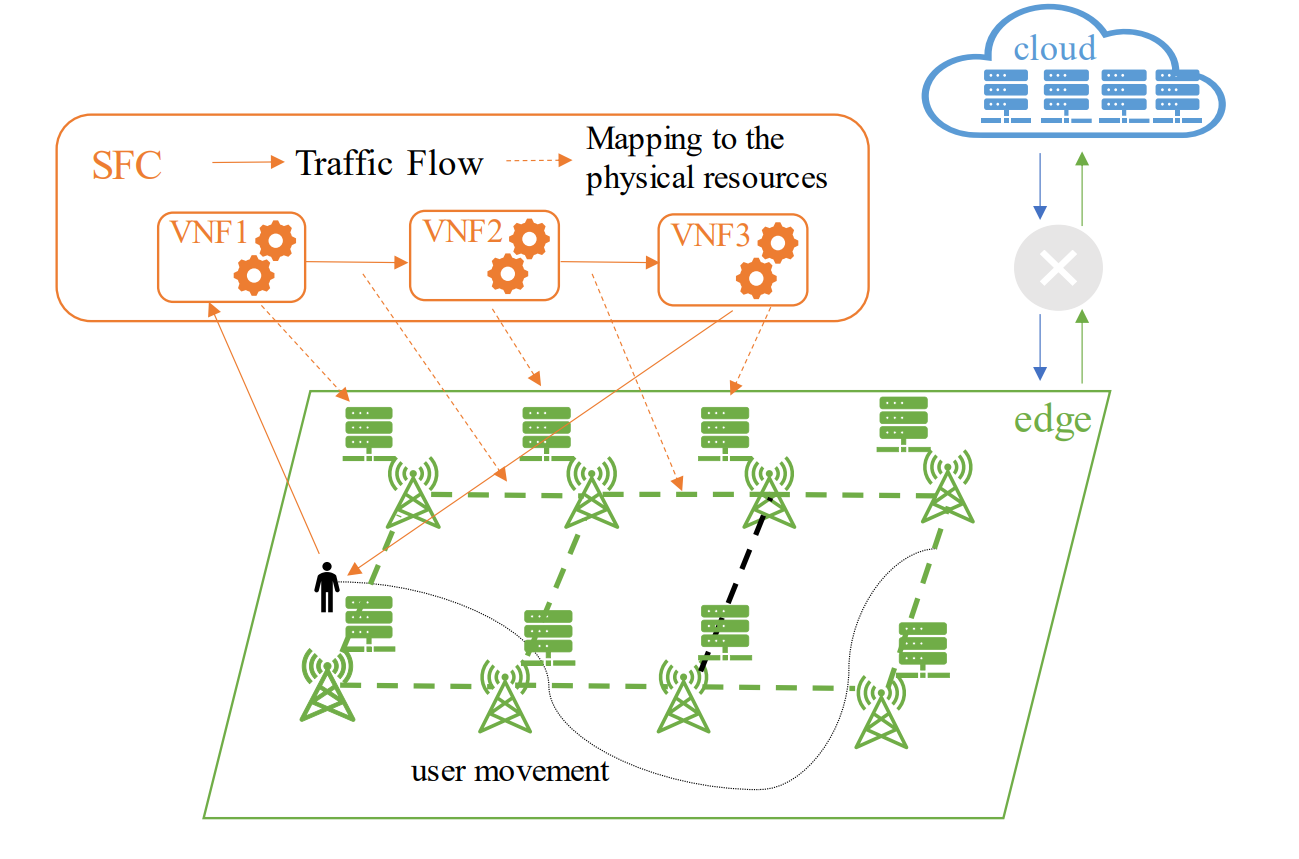
\includegraphics[width=0.9\linewidth]{figs/MEC_SFCdiagram_colored2.PNG}
		\vspace{\baselineskip}
	\caption{An example of SFC placement in MEC}
	\label{fig:mecsfcdiagram}
\end{figure}
\subsection{Network Model}
As illustrated in figure \ref{fig:mecsfcdiagram}, We consider a remote cloud $C$ and a mobile access network consisting of a set of base stations, each of which is bridged with an edge server, and is accessible through wireless channels.
Each base station is equipped with an edge server, where the set of all edge servers is denoted by $\mc{E}$. The cumulative processing capacity of the cloud and each edge server $e\in\mc{E}$ (in terms of the number of CPU cores) in timeslot $t$ is denoted, respectively, by $c_{C}(t)$ and $c_{e}(t)$\footnote{When cores are heterogeneous we must normalize the numbers with regard to the weakest CPU core in the system}. Edge servers are connected to each other and the remote cloud through a capacitated backbone network $G(\mc{R}, \mc{L})$, where $\mc{R}$ is the set of backbone routers and $\mc{L}$ is the set of backbone links. At time $t$, each link $\ell\in\mc{L}$ is associated with the bandwidth capacity $b_{\ell}(t)$ and propagation delay $d_{\ell}(t)$. We also refer to a link by its two endpoints, \eg, $d_{a,b}$ is the delay of the link between $a$ and $b$. Generally, the delay between edge servers and the cloud is significantly higher than the delay between edge servers. While, propagation delay within the cloud is considered to be negligible. 

\subsection{Service Model}
\label{sec:SFCrequest}
We assume that each user who roams in the vicinity of the access network has a mobile device $u$  (\eg\ Smartphone, tablet, in-vehicle infotainment system) with the processing capacity of $c_{u}(t)$, which is always connected to the nearest base station (denoted by $\beta$). Each user in time slot $t$ generates traffic at rate $\lambda(t)$ megabits per-second (Mbps) and requires it to be processed by a set of pre-determined \emph{services} in strict order (\aka\ a service chain). Each service is a software program (\eg\ video transcoder, firewall, and logger) that can be deployed in the cloud or an edge server with the means of state-of-the art virtualization methods such as Container~\cite{containerNFV}. We use $\mc{S}=(s_1, \dots, s_K)$ to denote the list of the user-required services and assume that service $s_i$ incurs $\pi_{s_{i}}$ seconds of delay to process $1$ Mbps of incoming data by using $1$ unit of CPU core. Moreover, each service can scale the user input traffic by a factor of $\alpha_{s_i}\in[0,\infty)$ before sending it to the next service due to operations such as encoding or decoding. Consequently, the traffic rate to the service $s_{i}$ can be computed by,
\begin{gather}
	\lambda_{s_{i}}(t) = \lambda(t) \times \prod_{j=1}^{i-1} \alpha_{s_j}.
\end{gather}
Note that service migration is inevitable as the user moves in the environment. Let $\mc{N}=\mc{E}\cup\{C, u\}$ represent all nodes that can host a service and provide the required processing capacity. The \textit{migration delay} $\rho_{a, b}^{s_{i}}(t)$
is defined as the time that the user has to wait for if her service $s_{i}$ is migrated from the source node $a$ to the destination node $b$ ($a,b \in \mc{N}$) in timeslot $t$ (clearly, $\rho_{a, a}^{s_{i}}(t)=0$). To serve a user request, each service in $\mc{S}$ should be deployed in a node with sufficient processing capacity, and the network routing should be adjusted such that user traffic goes through the services in the specified order. Finally, we assume that there is a special service at the end of the chain which is constrained to be placed on the user device. This technique guarantees that the results of the computation is carried back to the user.  

\begin{table}[t]
	\ra{1.2}
	\centering
	\caption{List of main notations in \myproblem\ formulation}
	\begin{tabular}{ll}
		\toprule
		Notation & \multicolumn{1}{c}{Description} \\
		\midrule
		$\mc{T}$ & Time frame \\
		$\mc{E}$ &  Set of all edge servers\\
		$C$ &  Cloud \\
		$\mc{L}$ &  Set of backbone links\\
		$\mc{R}$ & Set of backbone routers\\
		$b_{\ell}(t)$ & Current bandwidth capacity on link $\ell$\\
		$d_{\ell} (t)$ & Current propagation delay on link $\ell$ \\
		$c_{n}(t)$ & Current CPU core of node $n$ \\
		$\beta (t)$ & Current connected base station \\
		$\mc{S}$ & Set of all available services \\
		$\mc{N}$ & Set of all selectable nodes\\
		$\lambda(t)$ & Current user traffic rate \\
		$\pi_{s}$ & Processing delay factor of service $s$ \\
		$\alpha_{s}$ & Traffic scale factor of service $s$ \\
		$\rho_{a, b}^{s}(t)$ & Migration delay of service $s$ from node $a$ to node $b$ \\
		$\delta^{+}(r), \delta^{-}(r)$ & Incoming and outgoing links of router $r$\\
		%$\mc{C(t)}$ & Context \\
		%$\mc{S}(t)$ & SFC at time slot $t$ \\
		$x^s_n(t)$ & Current placement of service $s$ on node $n$\\
		$y^{s_i}_\ell(t)$ & Usage of link $\ell$ to route traffic from service $s_i$ to $s_{i+1}$  \\
		
		\bottomrule
	\end{tabular}
	\label{tab:System parameter}
\end{table}



\section{Problem Formulation}
\label{section: formulation}
In this section, we formally define the problem of SFC orchestration at the edge. Specifically, We consider the problem of service placement, service migration, and traffic routing with the objective of minimizing the user-perceived end-to-end delay. 
%We assume that users receive sophisticated feedback and manage manage their own services individually. This system operation scheme keeps the system complexity and scale at a smaller scale which enables us to achieve better solutions in later section. We call this the User-managed Edge-enabled Chain Placement Problem (\ie\ \myproblem).

\cat{Placement} To specify the placement of a service chain, we define binary decision variables $x_{n}^{s}(t)$, where $x_{n}^{s}(t)=1$ means that service $s$ is placed on the node $n$ in time slot $t$. We use the following constraint to ensure that every service in the chain is placed on a node,
\begin{gather}
	\sum_{n\in\mc{N}} x_{n}^{s}(t) = 1. 
	\qquad 
	\forall s\in\mc{S}, t\in\mc{T}
\end{gather}
Recent studies show that co-locating a user's services compromises the system reliability~\cite{colocatingService}. Thus, we include the following constraint to prevent co-located services,
\begin{gather}
	\sum_{s\in\mc{S}} x_{n}^{s}(t) \le 1. 
	\qquad 
	\forall n\in\mc{N}, t\in\mc{T}
\end{gather}

\cat{Routing}
A single path consisting of intermediate links and routers with enough bandwidth should be provisioned for every consecutive services $s_{i}$ and $s_{i+1}$ that are placed on separate nodes. To this end, we define binary decision variables $y_{\ell}^{s_{i}}(t)$, where $y_{\ell}^{s_{i}}(t)=1$ means that link $\ell$ is used to route the traffic between hosting nodes of services $s_{i}$ and $s_{i+1}$. Additionally, to unify the formulation and present it in a compact manner, we assume that a base station is a router and also assume that a hypothetical router resides on the user hand-held device the connects the device to the corresponding base station. We call this hypothetical router $\beta^{'}$ and denote the extended set of router by $\mc{R}^{'}=\mc{R}\cup\{\beta, \beta^{'}\}$. Therefore, we can use following constraint to specify a path,
\begin{gather}
	\textstyle\sum_{\ell\in\delta^{+}(r)} y_{\ell}^{s_{i}}(t)
	- \textstyle\sum_{\ell\in\delta^{-}(r)} y_{\ell}^{s_{i}}(t) = 0, \\
	\textstyle\sum_{\ell\in\delta^{-}(n)} y_{\ell}^{s_{i}}(t)
	- \textstyle\sum_{\ell\in\delta^{+}(n)} y_{\ell}^{s_{i}}(t)
	= x_{n}^{s_i} - x_{n}^{s_{i+1}},
\end{gather}
where, $\delta^{+}(r)$ and $\delta^{-}(r)$ show the incoming and outgoing links of router $r$,respectively. Furthermore, the following constraint is employed to ensure the capacity of links is respected,
\begin{gather}
	\sum_{s_{i}\in\mc{S}} \lambda_{s_{i+1}}(t)y_{\ell}^{s_{i}}(t) \le b_{\ell}(t).
	\qquad
	\forall \ell\in\mc{L}, t\in\mc{T}
\end{gather}

\cat{Delay}
The end-to-end chain delay is composed of four fundamental components: (1) \emph{processing delay}, (2)  \emph{transmission delay}, (3) \emph{propagation delay}, and (4) \emph{migration delay}. These delays, respectively, are represented by $\Gamma_{1}(t)$, $\Gamma_{2}(t)$, $\Gamma_{3}(t)$, and $\Gamma_{4}(t)$.
The total \emph{processing delay} is computed with regards to the traffic rate assigned to each services on SFC and the CPU cores of the nodes that each service is placed on, expressed as, 
\begin{gather}
	\Gamma_{1}(t) = \sum_{s\in\mc{S}} 
	\sum_{n\in\mc{N}} 
	\frac{x_{n}^{s}(t)\pi_{s}\lambda_{s}(t)}{c_{n}(t)}.
\end{gather}
The \emph{transmission delay} is computed with regards to the traffic rate routed to each link on SFC and its bandwidth,
\begin{gather}
	\Gamma_{2}(t) = \sum_{s_{i}\in\mc{S}} 
	\sum_{n\in\mc{N}} 
	\sum_{\ell\in \delta^{-}(r_n)} 
	\frac{y_{\ell}^{s_{i}}(t)\lambda_{s_{i+1}}(t)}{b_{\ell}(t)}.
\end{gather}
The \emph{propagation delay} of each link on SFC is computed as,
\begin{gather}
	\Gamma_{3}(t) = \sum_{s_{i}\in\mc{S}}
	\sum_{\ell\in\mc{L}} 
	y_{\ell}^{s_{i+1}}(t)d_{\ell}(t).
\end{gather}
Lastly, notice that when multiple services are migrated in the same timeslot, the transfer happens in parallel and thus the \emph{migration delay} is the maximum time that any of the re-located services need to start its operation. Consequently, the migration delay is computed as,
\begin{gather}
	\Gamma_{4}(t) = max\{
	\sum_{a,b\in\mc{N}}
	x_{a}^{s}(t-1)x_{b}^{s}(t)\rho_{a,b}^{s}(t)\}_{s\in\mc{S}}.
\end{gather}
As the objective, the user minimizes its overall weighted delay,
\begin{gather}
	\text{Min. }\sum_{t=0}^{\mathcal{T}} \sum_{i=1}^{4} \gamma_{i}\Gamma_{i}(t),
	\label{linearized obj}
\end{gather}
where, $\gamma_{i}$ are the scale factors that specifies the relative importance of the different components in the total delays $\Gamma_{i}$.



% \subsection{Placement strategy}
% In order to place a SFC on a network, we have to determine which node should we choose to place which kind of service. Thus, we use a binary variable $x^t_{i,s}$ to denote our placement decision at time slot $t$. $x^t_{i,s} = 1$ means that service $s$ will be placed on node $i$, the following constraints enforce that, for a given time slot, each service should be placed on one and only one node, each node can ran at most one service: 
%  \begin{equation}
%          x^t_{i,s}\in \{0,1\},\ \   \sum_{i\in \mathcal{M}} x^t_{i,s} = 1, \\ \sum_{s\in\mathcal{S} }x^t_{i,s} \leq 1.
% \end{equation}


% \subsection{Service demand}
% For different types of services (e.g. lightweight firewalls, Deep Packet Inspection and visual cloud computing), service demand can include memory, CPU and IO.  Here we use a simple model to characterize the overall capacity requirement of each service, more explicitly, the amount of capacity that is required by each service $s$ in the SFC at time slot $t$ is denoted by single variable $\lambda^t_s$, and we use a vector $\lambda^t$ to represent the sequential SFC demand, the order of the SFC $\mathcal{S}$ is followed in the demand vector and will be considered when making placement decisions. Therefore we have:
% \begin{equation}
%         \lambda^t = [\lambda^t_1, \lambda^t_2, ..., \lambda^t_s],\ \  s\in \mathcal{S}.
%     \end{equation}

% \subsection{Computing delay}
% At each time slot the user can choose a set of computing nodes to place the SFC on, and the computing delay will be sum of the computing latency of each service at time slot $t$ since the services will be executed in order, we use $c^t_i$ to denote the available computation capacity at node $i$ in that time slot and $\lambda^t_s$ represents the demand for service $S$ at time slot $t$ and $d^t_{cp}$ to denote the total computing delay, which is calculated by:
% \begin{equation}
%         d^t_{cp} = \sum_{s\in S}\sum\limits_{i\in M}x^t_{i,s} \frac{\lambda_s^t}{c^t_i}.
%   \end{equation}

%  \subsection{Communication delay}
%  We consider communication delay to be consisted of two parts: access latency between user and the base station, transfer delay between each services as the SFC is being processed. Thus the end-to-end delay will be calculated from sending SFC request to all the services being executed and returned to user from the last placed node. We use $f^t_{i, j}$ to denote the link capacity between two nodes. Due to earlier assumption that each computing node is connected with a based station, this will not only measures the access latency between the user current connected base station $l^t$ (depends on the location position) and base station of a computing node, it also measures the communication latency between two computing nodes $i$ and $j$. Therefore, the communication delay can be expressed as follow on a given SFC placement:
% %   \textbf{communication delay $d^m$}
%     \begin{equation}
%         d^t_{cm} =\sum_{s \in \mathcal{S}} \sum_{i\in M}\sum_{j\in M} f^t_{i,j}x^t_{i, s}x^t_{j, s+1} + \sum_{i\in M}x^t_{i, S[1]}  f^t_{l^t, i} +  \sum_{i\in M}x^t_{S[-1], i} f^t_{i, l^t},
%     \end{equation}
%   where $S[1]$ is the the first service and $S[-1]$ is the last service on the SFC,  
% \subsection{Switching cost}
% During the SFC placement at each time slot, the user may change the set of nodes to put services on, which will involve switching cost due to service migration. However, frequent service migration could cause a high failover and latency. Thus, we take switching cost into consideration in our model. The total switching cost would be the sum of migration cost over all services in the SFC at time slot $t$, we assume that for each service we also use the general model $f^t_{j, i}$ described in communication delay to measure the switching cost between computing node $i$ and $j$, the switch cost can be calculated as:
% \begin{equation}
%         S^t = \sum_{s\in S} \sum_{i\in M} \sum_{i\in M} f^t_{j,i} x^{t-1}_{j, s} x^{t}_{i,s},
%     \end{equation}
% specifically, we assume that for nodes on the cloud, the switching cost between them is negligible and the switching cost between the cloud node and edge node will be considerably larger.
% \subsection{Objective}
% To optimize the SFC cost in a balanced manner, we formulate the total SFC cost minimization with weight on each cost and define the objective service cost as follow:
%   \begin{equation}
%          Cost(t) = \sum\limits _{t\in \mathcal{T}} w^t_1d^t_{cp} + w^t_2d^t_{cm} + w^t_3s^t.
%   \end{equation}

%  Where $w_1^t$, $w_2^t$ and $w_3^t$ are the dynamic weights of computing delay, communication delay and switching cost.


\section{Complete Problem Formulation}
\label{section: complete problem formulation}
In an offline setting, given the network topology and delays, demands, user's location at each time slot, our goal is to find a sum minimum delay throughout all time slots while satisfying the constraints for link bandwidth and co-located services prevention. 
We note that sub-objective~\ref{linearized obj} in the above formulation is non-linear. In this section, we show how to linearize it and formulate the problem above into a binary integer programming (BIP) that can be solved using standard solvers such as Gurobi\cite{gurobi}, which allow us to get an offline optimum as a performance benchmark.

The last sub-objective $\Gamma_4(t)$ contains a product of two binary variables: $x^s_a(t-1)$ and $x^s_b(t)$, which can be replaced by introducing a 2-dimension multiplication binary variables $x^s_{a,b}(t)$ and several equivalent linearized constraints, we can rewrite objective~\ref{linearized obj}  as follows:
\begin{equation}
	\label{eqn:objlinearization}
	\begin{aligned}
		&\Gamma_{4}(t) = \sum_{s\in\mc{S}}
		\sum_{a,b\in\mc{N}}
		x^s_{a,b}(t)\rho_{a,b}^{s}(t),\\
		&x^s_{a,b}(t) = x^s_a(t-1) * x^s_b(t),\\
		& x^s_{a,b}(t) \leq x^s_a(t-1), \\
		&x^s_{a,b}(t) \leq x^s_b(t),\\
		& x^s_{a,b}(t)  \geq  x^s_a(t-1) + x^s_b(t) -1,\\
		& \forall t\in \mathcal{T}, \forall s \in \mathcal{S}, \forall a,b \in \mathcal{N}.\\
	\end{aligned}
\end{equation}
% We note that that equation (4) and (5) contains a product of two binary variables: $x^t_{i, s}x^t_{j, s+1}$ and $x^{t-1}_{j, s} x^{t}_{i,s}$, which can be linearized by introducing two multiplication binary variables $xs_{i,j,s,t}$ and $xt_{i, j, s ,t}$ and equivalent linearized constraints, we hence reformulate it into a linear objective as follow:

% \begin{equation}
% \begin{aligned}
%     &xs^t_{i,j,s} = x^t_{i, s}x^t_{j, s+1},\\
%     &xt^t_{i, j, s} = x^{t-1}_{j, s} x^{t}_{i,s},\\
%     & xs^t_{i,j,s} \leq x^t_{i, s}, xs^t_{i,j,s}\leq x^t_{j, s+1}, xs^t_{i,j,s}\geq x^t_{i, s} + x^t_{j, s+1} - 1,\\
%     & xt^t_{i, j, s} \leq x^{t-1}_{j, s}, xt^t_{i, j, s} \leq x^{t}_{i,s}
%     xt^t_{i, j, s}  \geq  x^{t-1}_{j, s} + x^{t}_{i,s} -1,\\
%     & \forall t\in \mathcal{T}, \forall s \in \mathcal{S}, \forall i,j \in \mathcal{M}.\\
% \end{aligned}
% \end{equation}

% Our offline algorithm that solve the problem using a BIP formulatiom is given in algorithm 1
Formulation \ref{formulation:offline} presents the complete problem formulation for the offline placement in the form of a BILP



\begin{problemenv}
	\caption{Exact offline \myproblem}
	\label{formulation:offline}
	\begin{equation}
		\begin{array}{ll@{}ll}
			\text{Min.}   & \sum\limits_{t=0}^{\mathcal{T}} \sum\limits_{i=1}^{4} \gamma_{i}\Gamma_{i}(t)\\
			\text{s.t.} 
			&\Gamma_{1}(t) = \sum\limits_{s\in\mc{S}} 
			\sum\limits_{n\in\mc{N}} 
			\frac{x_{n}^{s}(t)\pi_{s}\lambda_{s}(t)}{c_{n}(t)}.\\
			&    \Gamma_{2}(t) = \sum\limits_{s_{i}\in\mc{S}} 
			\sum\limits_{n\in\mc{N}} 
			\sum\limits_{\ell\in \delta^{-}(r_n)} 
			\frac{y_{\ell}^{s_{i}}(t)\lambda_{s_{i+1}}(t)}{b_{\ell}(t)}.\\
			&\Gamma_{3}(t) = \sum\limits_{s_{i}\in\mc{S}}
			\sum\limits_{\ell\in\mc{L}} 
			y_{\ell}^{s_{i+1}}(t)d_{\ell}(t).\\
			&\Gamma_{4}(t) = \sum_{s\in\mc{S}}
			\sum_{a,b\in\mc{N}}
			x^s_{a,b}(t)\rho_{a,b}^{s}(t).\\
			&    \sum\limits_{n\in\mc{N}} x_{n}^{s}(t) = 1. 
			\qquad 
			\forall s\in\mc{S}, t\in\mc{T}.\\
			& \sum\limits_{s\in\mc{S}} x_{n}^{s}(t) \le 1. 
			\qquad 
			\forall n\in\mc{N}, t\in\mc{T}.\\
			&\sum\limits_{\ell\in\delta^{+}(r)} y_{\ell}^{s_{i}}(t)
			- \sum\limits_{\ell\in\delta^{-}(r)} y_{\ell}^{s_{i}}(t)
			= x_{n_r}^{s_{i}}(t) - x_{n_r}^{s_{i+1}}(t).
			\qquad \\
			&\qquad\qquad\qquad\qquad\qquad\qquad\qquad\forall r \in\mc{R}^{'},t\in\mc{T}.\\
			&  \sum\limits_{s_{i}\in\mc{S}} \lambda_{s_{i+1}}(t)y_{\ell}^{s_{i}}(t) \le     b_{\ell}(t).
			\qquad
			\forall \ell\in\mc{L}, t\in\mc{T}.\\
			& x^s_{a,b}(t) \leq x^s_a(t-1), \\
			&x^s_{a,b}(t) \leq x^s_b(t),\\
			& x^s_{a,b}(t)  \geq  x^s_a(t-1) + x^s_b(t) -1,\\
			& \forall t\in \mathcal{T}, \forall s \in \mathcal{S}, \forall a,b \in \mathcal{N}.\\     
			% & xs^t_{i,j,s} \leq x^t_{i, s}, xs^t_{i,j,s}\leq x^t_{j, s+1}, xs^t_{i,j,s}\geq x^t_{i, s} + x^t_{j, s+1} - 1,\\
			% & xt^t_{i, j, s} \leq x^{t-1}_{j, s}, xt^t_{i, j, s} \leq x^{t}_{i,s}
			% xt^t_{i, j, s}  \geq  x^{t-1}_{j, s} + x^{t}_{i,s} -1,\\
			% & \forall t\in \mathcal{T}, \forall s \in \mathcal{S}, \forall i,j \in \mathcal{M},\\
			
			&\text{constants}:\gamma,  \pi, \lambda, \rho, c, b, \mathcal{T}, \mathcal{N}, \mathcal{S}, \mathcal{L}\\
		\end{array}
	\end{equation}
\end{problemenv}


\chapter{\textbf{Proposed Method}}
\label{chapter: Proposed Method}
In this chapter, we present the design of \myalgorithm, our proposed bandit-based algorithm for online SFC orchestration at the edge.

We first present the contextual combinatorial bandit formulation~\cite{C^2MAB} of the chain placement problem by characterizing the environment with a set of \emph{arms} (\ie\ placement options) and specifying their relations in subsection~\ref{section_bandit_formulation}.
The formulation reduces the bandit solution's computational complexity and allows the user to handle the uncertainty in the environment and through repeated interactions to find efficient service placement and resource allocation schemes. Specifically, the context allows the user to incorporate the available information into the resource allocation procedure (\eg\ demand). The combinatorial formulation allows the user to focus on the primitive options (\ie\ servers and links) during the learning procedure, which significantly reduces the problem space. Otherwise, the user would be forced to consider all the solutions, which are exponential in terms of the number of servers and links (\eg\ all the different paths in the network). 
Then, we show how to reduce the uncertainty about the quality
of arms and use the result to compute a service efficiently
placement by dynamic programming, which is presented in subsection~\ref{sec:placement algorithm}


%In this section, we present the design of \myalgorithm, our proposed bandit-based algorithm for online SFC orchestration at the edge. To reduce the computational complexity of the bandit solution, we apply the contextual bandit formulation~\cite{C^2MAB} by characterizing the environment with a set of \emph{arms} (\ie\ placement options) and specifying their relations in subsection~\ref{section_bandit_formulation}.
%%
%Then, we show how to reduce the uncertainty about the quality of arms and use the result to efficiently compute a service placement by dynamic programming in subsection~\ref{subsection_dynamic_programming}.


\subsection{Bandit Formulation}
\label{section_bandit_formulation}
At the beginning of each timeslot $t$,
user-side information such as their service demands $\lambda(t)$ during the timeslot, the current location $\beta(t)$, and the placement of their service chain in the previous timeslot(\ie\ $x_n^s(t-1)$) is known. In contrast, the system-level information such as processing and bandwidth capacity of servers and links are not accessible, thereby are required to be learned by the user. 
%
Therefore, to learn about the environment, we consider each server and link as an option that can be used for placing a service, which is analogous to the concept of \emph{arm} in bandit theory. The available options in each timeslot are defined to be $O_{t}\subseteq \mc{L}\cup\mc{N}$, which is the set of all links, user's device, edge servers, and the remote cloud. At the beginning of each timeslot, based on the information learned so far, the user selects a subset of feasible options for the service chain's placement and minimizes the end-to-end delay. At the end of each timeslot, the user observes each option's contribution to the delay objective. Specifically, for each selected option $o\in O_{t}$, the user observes some value $\delta_{o}(t)$. This value is only a noisy estimate of the true value of the option $o\in O_{t}$. Our goal is to quickly and efficiently estimate the true values of delays incurred by each option.
%
According to our delay formulation, each option contributes \emph{linearly} to the user's perceived end-to-end delay. Following the framework of contextual bandits, we assume that in each timeslot $t$, the significance of each option depends only on an unknown system parameter vector $\theta$ and a contextual feature vector $\pmb{\chi}_{o}(t)$ that is fully known to the user. For example, the edge server capacities are unknown parameters but the user's current location is a known contextual feature.
%
Thus, the observed value $\delta_{o}(t)$ is characterized as follows:
\begin{gather}
	\delta_{o}(t) = \theta^{\intercal} \times \pmb{\chi}_{o}(t) + \epsilon_{o}(t),
\end{gather}
where, $\epsilon_{o}(t)$ is a zero-mean random variable representing the noise delay in the network. 
%

Note that the user can select arm $o$ as a part of service placement resources but only observes the resulting delay $\delta_{o}(t)$ at the end of the timeslot. Specifically, the user, in each timeslot, using the historical information, should select a subset of options $O_{t}\subseteq \mc{L}\cup\mc{N}$ that (1) is feasible for the placement of the service chain and (2) minimizes the overall delay perceived by the user. The user's goal is to minimize the expected cumulative delay in the period of service placement, which is defined as,
\begin{gather}
	\mathbb{E}\left[\sum_{t\in\mc{T}} \sum_{o\in O_{t}} \delta_{o}(t)\right].
\end{gather}

In the following, we fully describe the system parameter vector
$\theta$ and contextual feature vector $\pmb{\chi}_{o}(t)$.

\cat{System Parameters}
The parameter vector of the system (which is unknown to the user) is composed of four sub-vectors, where each sub-vector contains parameters that are related to a specific type of delay.
\begin{enumerate}[leftmargin=*]
	\item $\theta_{c}$ is the sub-vector of parameters that determine the processing delay based on the number of CPU cores in each computing node:
	\begin{gather}
		\theta_{c} = [\textstyle\frac{1}{c_{n}}, \quad \forall n\in\mc{N}]. 
	\end{gather}
	\item $\theta_{b}$ is the sub-vector of parameters that determine the transmission delay based on the bandwidth of links:
	\begin{gather}
		\theta_{b} = [\textstyle\frac{1}{b_{\ell}}, \quad \forall \ell\in\mc{L}].
	\end{gather}
	\item $\theta_{d}$ is the sub-vector of parameters that determine the propagation delay:
	\begin{gather}
		\theta_{d} = [d_{\ell}, \quad \forall \ell\in\mc{L}].
	\end{gather}
	\item $\theta_{\rho}$ is the sub-vector of parameters that determine the service migration delay:
	\begin{gather}
		\theta_{\rho} = [\rho_{a,b}^{s}, \quad \forall a,b\in\mc{N}, s\in\mc{S}].
	\end{gather}
\end{enumerate}
Finally, it is possible to construct the system parameter vector $\theta$ from the concatenation of the aforementioned sub-vectors:
\begin{gather}
	\theta = \theta_{c} \oplus \theta_{b} \oplus \theta_{d} \oplus \theta_{\rho},
\end{gather}
where, $\oplus$ is the concatenation operator.


\cat{Notation}
In the following, we use the notation $1_p$ to represent an indicator function that is equal to $1$ when the logical predicate $p$ is true and is equal to $0$ otherwise. 

\cat{Contextual Features}
We define a contextual feature vector to represent the known information at the user's side for each placement option $o\in O_t$. Each option is either a link $o=\ell\in\mc{L}$ or a computation node $o=n\in\mc{N}$. Since the information about links and nodes are different, we define a feature vector for nodes and links separately. The contextual vector, similar to the parameter vector, comprises four sub-vectors that correspond to four types of delay. The link contextual sub-vectors are defined as follows:
\begin{enumerate}[leftmargin=*]	
	\item $\pmb{\chi}_{\ell}^{b}(t)$ is the sub-vector corresponding to the transmission delay. $\pmb{\chi}_{\ell}^{b}(t)$ contains contextual information about the user's transmission rate.
	\begin{gather}
		\pmb{\chi}_{\ell}^{b}(t) = [1_{\ell'=\ell,\exists n\in\mc{N}: \ell'\in \delta^{-}(n)}\lambda_{s}(t), \quad \forall \ell'\in\mc{L}].
	\end{gather}
	Note that if the user uses link $\ell$ to transfer the result of computation out of the computation node $n$, the multiplication of this sub-vector by the system parameter vector computes the expected transmission delay.
	\item When the user selects a link, its corresponding propagation delay is incurred. Thus, the contextual propagation delay sub-vector of link $\ell$, denoted by $\pmb{\chi}_{\ell}^{d}(t)$, is defined as:
	\begin{gather}
		\pmb{\chi}_{\ell}^{d}(t) = [1_{\ell'=\ell}, \quad \forall \ell'\in\mc{L}],
	\end{gather}
	Note that when this sub-vector is multiplied by the corresponding system sub-vector the propagation delay of $\ell$ is obtained.
	
	\item Since links have no effect on the computational and migration delays, the corresponding sub-vectors, denoted by $\pmb{\chi}_{\ell}^{c}(t)$ and $\pmb{\chi}_{\ell}^{\rho}(t)$, respectively, are zero vectors:
	\begin{gather}
		\pmb{\chi}_{\ell}^{c}(t) = [0, \quad \forall n\in\mc{N}], \\
		\pmb{\chi}_{\ell}^{\rho}(t) = [0, \quad \forall a,b\in\mc{N}, s'\in\mc{S}].
	\end{gather}
\end{enumerate}
Thus, the contextual feature vector of each link $\ell$ that is going to be used to route the traffic towards service $s\in\mc{S}$ is obtained from the concatenation of these sub-vectors:
\begin{gather}
	\pmb{\chi}_{\ell}(t) = \pmb{\chi}_{\ell}^{c}(t) \oplus \pmb{\chi}_{\ell}^{b}(t) \oplus \pmb{\chi}_{\ell}^{d}(t) \oplus \pmb{\chi}_{\ell}^{\rho}(t), 
\end{gather}
The contextual feature vector of each computation node is defined based on four sub-vectors as follows:
\begin{enumerate}[leftmargin=*]
	\item The contextual sub-vector of computation features, denoted by $\pmb{\chi}_{n}^{c}(t)$, is defined as follows: 
	\begin{gather}
		\pmb{\chi}_{n}^{c}(t) = [1_{n'=n}\times \pi_{s}\lambda_{s}(t), \quad \forall n'\in\mc{N}].
	\end{gather}
	Note that if we multiply this sub-vector by the sub-vector of system parameters for computation, the computation delay of running the service $s$ on node $n$ is obtained.
	\item The migration contextual sub-vector contains information about the placement of services in the previous timeslot.  We denote this sub-vector by $\pmb{\chi}_{n}^{\rho}(t)$ and define it as follows:
	\begin{gather}
		\pmb{\chi}_{n}^{\rho}(t) = [1_{s'=s,b=n}x_{a}^{s}(t-1), \quad \forall a,b\in\mc{N}, s'\in\mc{S}].
	\end{gather}
	%\hl{	Note that this sub-vector }
	\item Since computation nodes do not affect the transmission and propagation delays, the corresponding contextual feature sub-vectors, denoted by $\pmb{\chi}_{n}^{b}(t)$ and $\pmb{\chi}_{n}^{d}(t)$, respectively, are zero vectors: 
	\begin{gather}
		\pmb{\chi}_{n}^{b}(t) = [0, \quad \forall \ell\in\mc{L}], \\
		\pmb{\chi}_{n}^{d}(t) = [0, \quad \forall \ell\in\mc{L}].
	\end{gather}
\end{enumerate}
Finally, the contextual feature of each node $n$ where service $s\in\mc{S}$ is placed is obtained by concatenating the mentioned sub-vectors:
\begin{gather}
	\pmb{\chi}_{n}(t) = \pmb{\chi}_{n}^{c}(t) \oplus \pmb{\chi}_{n}^{b}(t) \oplus \pmb{\chi}_{n}^{d}(t) \oplus \pmb{\chi}_{n}^{\rho}(t), 
\end{gather}


\subsection{Placement Algorithm}
\label{sec:placement algorithm}
In this subsection, we present the design of our proposed bandit-based algorithm that efficiently estimates each arm's value, which is equivalent to the expected delay of each placement option.
Our proposed bandit-based algorithm for SFC placement on edge is summarized in Algorithm~\ref{alg:cccpa}, called \myalgorithm.
\myalgorithm\ repeatedly examines different placement strategies and adjusts the estimates based on the noisy feedback it receives from the system. Then, \myalgorithm\ uses the expected estimated delay values to compute a placement with the minimum end-to-end delay. \myalgorithm\ is outlined in  Algorithm~\ref{alg:cccpa}. \myalgorithm\ gets the service chain, the contextual features, and available nodes and links as the input. To estimate the expected delay for each placement option, the algorithm has to estimate the system parameter vector $\theta$. We use $\hat{\theta}(t)$ and $\hat{\delta}_o(t)$ to represent the estimated parameter vector and estimated delay for placement option $o$ at timeslot $t$. To compute these values, we applied the confidence bound-based algorithm in~\cite{C^2MAB}.

The algorithm starts with an initial estimate for the covariance matrix  $\pmb{V}_{0}$ and mean vector $\pmb{b}_{0}$ of system parameters expressed as follows (line~\ref{alg_bandedge_line_V0}-\ref{alg_bandedge_line_b0}),
\begin{gather}
	\pmb{V}_{0} \gets \pmb{I}_{d\times d}, \label{eqn:v_init} \\

	\pmb{b}_{0} \gets \pmb{0}_{d}, \label{eqn:b_init}.\end{gather}

In each timeslot, the estimated system parameter vector is obtained from the covariance matrix and the mean vector. The estimated system parameter vector is then used to compute the excepted delay of each placement option, which is expressed as follows (line~\ref{alg_bandedge_line_theta}-\ref{alg_bandedge_line_delta_bar}), 
\begin{gather}
	\hat{\theta}(t)
	\gets
	\pmb{V}_{t-1}^{-1}\pmb{b}_{t-1}, \label{eqn:theta_hat}\\
	\bar{\delta}_{o}(t)
	\gets
	\hat{\theta}(t)^{\intercal}
	\pmb{\chi}_{o}(t), \forall o \in O_t.
\end{gather}
Then, a lower bound for each delay values in computed as follows (line~\ref{alg_bandedge_line_delta_hat}),
\begin{gather}
	\hat{\delta}_{o}(t)
	\gets
	\bar{\delta}_{o}(t)
	-
	\sqrt{\pmb{\chi}_{o}(t)^{\intercal}\pmb{V}_{t}^{-1}\pmb{\chi}_{o}(t)}. 
	\label{eqn:delta_hat}
\end{gather}

Then, the algorithm selects a set of placement options $P_{t}$ at time $t$ based on a placement strategy, which is expressed as follows(line~\ref{alg_bandedge_line_place}),
\begin{gather}
	P_{t}\leftarrow \textbf{Place}(\hat{\delta}_{o}(t), \mc{S}[t]).
\end{gather}
The placement strategy, based on dynamic programming, is outlined in Algorithm~\ref{alg:DP_SFC}.

Finally, the computed placement is implemented and the algorithm observes the delay values
incurred as a result. The algorithm the update the covariance matrix
and the mean vector accordingly as follows (line~\ref{alg_bandedge_line_update_V}-\ref{alg_bandedge_line_update_b}),
\begin{gather}
	\pmb{V}_{t} \gets \pmb{V}_{t-1} + \sum_{{o}\in P_{t}} \pmb{\chi}_{o}(t)\pmb{\chi}_{o}(t)^{\intercal}, \label{eqn:v_update}\\
	\pmb{b}_{t} \gets \pmb{b}_{t-1} + \sum_{{o}\in P_{t}} \delta_{o}(t)\pmb{\chi}_{o}(t).\label{eqn:b_update}
\end{gather}
%The user, then, uses $\pmb{V}_{0}$ and $\pmb{b}_{0}$ as follows to compute new lower-bound estimates,
%\begin{gather}
%\hat{\theta}(t)
%\gets
%\pmb{V}_{t}^{-1}\pmb{b}_{t}, \label{eqn:theta_hat} \\
%\bar{\delta}_{n}(t)
%\gets
%\hat{\theta}(t)^{\intercal}
%\pmb{\chi}_{n}(t), \\
%\hat{\delta}_{n}(t)
%\gets
%\bar{\delta}_{n}(t)
%-
%c\sqrt{\pmb{\chi}_{n}(t)^{\intercal}\pmb{V}_{t}^{-1}\pmb{\chi}_{n}(t)}, \label{eqn:delta_hat}
%\end{gather}

\cat{Exploration vs Exploitation}
In online learning, \textit{Exploration} allows user to improve their knowledge about each arm that is likely to lead to a long-term benefit while \textit{Exploitation} allows user to exploit their current knowledge by choosing the current largest estimated arms. In equation~\ref{eqn:delta_hat}, $\bar{\delta}_{n}(t)$ denotes the current estimates at timeslot $t$ and therefore represent the exploitation, while $\sqrt{\pmb{\chi}_{n}(t)^{\intercal}\pmb{V}_{t}^{-1}\pmb{\chi}_{n}(t)}$ denotes the adjustment made on each arm and therefore represent exploration. Additionally, we associate
a constant ratio $c$ to exploration term to determine the exploration-exploitation level, refer to as \textit{exploration ratio}.\ \eg, bigger $c$ leads to a smaller lower bound on the estimates and encourages exploration, smaller $c$ leads to a larger lower bound and encourages exploitation. We further evaluate the effect of the exploration ratio $c$ in section~\ref{eval:explorationratio}.
\begin{algorithm}[t]
	%\fontsize{12}{12}\selectfont
	\DontPrintSemicolon
	\caption{\textbf{\myalgorithm}: \textbf{Cha}i\textbf{n} Orchestrator at the Ed\textbf{ge}}
	\label{alg:cccpa}
	\SetKwInput{kwInit}{Init}
	\textbf{Input}: $\mc{N}, \mc{L}, \mc{S},\pmb{\chi} $\\
	$\pmb{V}_{0} \gets \pmb{I}_{d\times d}$ \label{alg_bandedge_line_V0} \\
	$\pmb{b}_{0} \gets \pmb{0}_{d}$ \label{alg_bandedge_line_b0} \\
	\For{$t\in \mc{T}$}{
		$\hat{\theta}(t)
		\gets
		\pmb{V}_{t-1}^{-1}\pmb{b}_{t-1}$ \label{alg_bandedge_line_theta} \\
		$\bar{\delta}_{o}(t)
		\gets
		\hat{\theta}(t)^{\intercal}
		\pmb{\chi}_{o}(t), \forall o \in O_t$ \label{alg_bandedge_line_delta_bar} \\
		$\hat{\delta}_{o}(t)
		\gets
		\bar{\delta}_{o}(t)
		-
		\sqrt{\pmb{\chi}_{o}(t)^{\intercal}\pmb{V}_{t}^{-1}\pmb{\chi}_{o}(t)}$ \label{alg_bandedge_line_delta_hat} \\
		$P_{t}\leftarrow \textbf{Place}(\hat{\delta}_{o}(t), \mc{S}[t])$ \label{alg_bandedge_line_place} \\
		$\pmb{V}_{t} \gets \pmb{V}_{t-1} + \sum_{{o}\in P_{t}} \pmb{\chi}_{o}(t)\pmb{\chi}_{o}(t)^{\intercal}$ \label{alg_bandedge_line_update_V} \\
		$\pmb{b}_{t} \gets \pmb{b}_{t-1} + \sum_{{o}\in P_{t}} \delta_{o}(t)\pmb{\chi}_{o}(t)$ \label{alg_bandedge_line_update_b} \\
	}
\end{algorithm}

%\cat{Proposed Algorithm} Our proposed bandit based algorithm for SFC placement on Edge is summarized in Algorithm~\ref{alg:cccpa}, we call it \textit{\myalgorithm} 
\cat{SFC placement algorithm}The SFC placement algorithm, presented in Algorithm~\ref{alg:dplace} is based on the dynamic programming (DP) principle, which, given the delay estimates $\hat{\delta}_{o}(t)$ and required service set $\mc{S}[t]$,  calculates the optimal resource allocation in polynomial time by defining the cost of an optimal solution recursively in a bottom-up fashion. DP finds the optimal solution by starting from placing one single service and successively moving to next service while taking the previous solutions into account. There are three recurrence relations for the minimum cost to place service $s_{i}$ on node $j$ as explained below (line 5-12):
\begin{itemize}[leftmargin=*]
	\item $s_{i}$ is the first service on SFC:
	\begin{equation}
		\widetilde{D}(s_{i}, j) = \hat{\delta}_{l_{\beta(t), j}(t)} +  \hat{\delta}_j(t) %+ s(s_{i}, j) \\
		+ min\{\hat{\delta}_{l_{j, k}}(t) + \widetilde{D}(s_{i+1}, k)\}_{k\in \mathcal{N}}.
		%	d(s_{i}, j) = \hat{\delta}_{l_{g, j}}(t) + d_{cp}(s_{i}, j) + s(s_{i}, j) \\
		%	+ min\{d_{cm}(j, k) + \text{Cost}(s_{i+1}, k)\}_{k\in \mathcal{N}}.
	\end{equation}
	\item $s_{i}$ is the last service on SFC:
	\begin{equation}
		\widetilde{D}(s_{i}, j) =  \hat{\delta}_j(t)+\hat{\delta}_{l_{j, \beta(t)}}(t)
		%\text{Cost}(s_{i}, j) = d_{cp}(s_{i}, j) + s(s_{i}, j) + d_{cm}(j, g)
	\end{equation}
	\item $s_{i}$ is neither the first and nor the last service on SFC:
	\begin{equation}
		\widetilde{D}(s_{i}, j) =  \hat{\delta}_j(t) 
		+ min\{\hat{\delta}_{l_{j, k}}(t) + \widetilde{D}(s_{i+1}, k)\}_{k\in \mathcal{N}}.
	\end{equation}
\end{itemize}
The optimal placement of a SFC is then determined by the node with the minimum cost to place the first service, that is:
\begin{equation}
	\text{Cost}(\text{SFC}) = min\{\text{Cost}(1,n)\}_{n\in\mc{N}}.
\end{equation}
The solution is obtained by extracting the host list associate with it, that is:
\begin{equation}
	P_{t}\leftarrow H(1, n)
\end{equation}
%where  $d_{cm}(s_{i},j)$ denotes the computing delay of vnf $s_{i}$ on node $j$, $d_cm(s_{i},j)$ denotes the link delay between node $i$ and node $j$ and $s(i,j)$ denotes the switching cost from node $i$ to $j$, $g = \beta(t)$, which indicates the user's current connected base station. 

\begin{algorithm}[t]
	%\fontsize{8}{8}\selectfont
	\DontPrintSemicolon
	\caption{\textbf{Place}($\hat{\delta}_{o}(t)$, $\mc{S}[t]$)}
	\label{alg:dplace}
	\SetKwInput{kwInit}{Init}
	$H(i,j) \leftarrow \mathbf{0} \quad \forall i\in \mc{S}[t], \forall j\in \mc{N}$ \\
	$\widetilde{D}(s_i,j)\leftarrow 0 \quad \forall i\in \mc{S}[t], \forall j\in \mc{N}$ \\
	\For{$i \in S..1$}{
		\ForEach{$j \in \mc{N} $}
		{
			\eIf{$i = 1$}{
				$\widetilde{D}(s_{i}, j) = \hat{\delta}_{l_{\beta(t), j}(t)} +  \hat{\delta}_j(t)
				+ min\{\hat{\delta}_{l_{j, k}}(t) + \widetilde{D}(s_{i+1}, k)\}_{k\in \mathcal{N}}.$
				
			}
			{
				\eIf{$i=S$}{
					$\widetilde{D}(s_{i}, j) =  \hat{\delta}_j(t)+\hat{\delta}_{l_{j, \beta(t)}}(t)$}
				{$\widetilde{D}(s_{i}, j) =  \hat{\delta}_j(t) 
					+ min\{\hat{\delta}_{l_{j, k}}(t) + \widetilde{D}(s_{i+1}, k)\}_{k\in \mathcal{N}}.$}}
			$H(i,j) \leftarrow H(i-1, k).append(k)$
		}     
	}
	Extract the node with the minimum cost to place $s_1$: $n \leftarrow \text{argmin}\{\widetilde{D}(s_1, j)\}_{j \in \mathcal{N}}$ \\
	Get the corresponding host list as the solution $P_{t}\leftarrow H(1, n)$ \\
	\textbf{Return} $P_t$
\end{algorithm}          
With probability $1-\epsilon$, the regret of the proposed  algorithm is less than 
\begin{equation}
	O(Slog(n)\sqrt{T}+\sqrt{TSlog(T/\epsilon)}),
\end{equation}
where, $S$ shows the length of the chain and $T$ is the lifetime of the chain (\ie\ total timeslot). For detailed analysis refer to \cite{C^2MAB}.

\begin{theorem}
	With combinatorial bandit formulation, the decision space of the user is reduced by the following factor compared to a general bandit formulation:
	\begin{gather}
		\label{eqn: decision space}
		\frac
		{n + l}
		{\sum_{k = 0,...,s} \frac{n!s!}{k!(s-k)!(n-s+k)!}}
	\end{gather}
	
\end{theorem}
\begin{proof}
	A general Combinatorial Multi-armed Bandit (CMAB) algorithm selects the arm (a set of underlying arms) of round t to play based on the outcomes of revealed arms selected in previous rounds, without knowing the expectation vector $\mu$ of all individual arms \cite{chen2013combinatorial}. 
	We denote $S_t$ to be the super arm selected in round t, which can be a random super arm chosen depending on the outcomes of arms in previous rounds and potential randomness in the algorithm itself. 
	The objective of CMAB is to maximize the expected reward of all rounds up to round n, that is, Min$(\E_S[\sum_{t\in\mc{T}} r(S_t)])$, where $\E_S$ denotes taking expectation only among all random events generating the super arm $ S_t$'s, $r(S_t)$ is a non-negative variable denoting the reward of round $t$ when super arm $S$ is played.
	In order to formulate the \myproblem\ into a general CMAB problem, the size of the arm set that the user can choose can be analyzed as follow, during each timeslot, the user is presented with the choice of selecting a set of nodes from mobile edge or cloud to deploy SFC and run applications. Therefore we define a set of nodes as a super arm. For example, we consider $n$ edge nodes, $l$ links, one cloud in the MEC network, and $s$ service requested. Since in the core network, the computing resources are considered to be limitless and are capable of running all the services, we assume that there are at least $s$ nodes to choose from in the cloud, by combinations the total decision space can be calculated as the bottom part of eq.\ref{eqn: decision space}. With our proposed CMAB formulation, the decision space is reduced to $n + l$ because we view individual links and nodes as candidates to select.  
\end{proof}

\begin{figure}[t]
	\centering
	\begin{subfigure}[b]{.48\linewidth}
		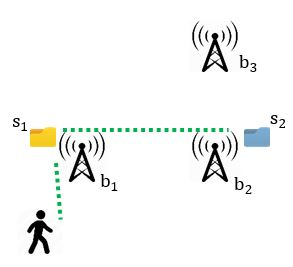
\includegraphics[width=0.7\linewidth]{figs/example_before.JPG}
		\caption{Service placement at $T_1$}
		\label{fig:alg_example_before}
	\end{subfigure}
	\hfill
	\begin{subfigure}[b]{.48\linewidth}
		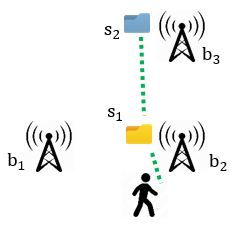
\includegraphics[width=0.7\linewidth]{figs/example_after.JPG}
		\caption{Service placement at $T_2$}
		\label{fig:alg_example_after}
	\end{subfigure}
	\vspace{\baselineskip}
	\caption{An illustrative example used for CMAB formulation}
	
	\label{fig:algo_example}
\end{figure}

\subsection{Bandit Formulation Example}
Assume there are $3$ base stations as shown in Fig.~\ref{fig:algo_example}. At time $T_1$, the user is in the vicinity of $b_1$. The first service $s_1$ is located in the edge server at $b_1$ and the second service $s_2$ is located in the edge server at $b_2$. Assume that after some time the user moves to the neighborhood of the base station $b_2$ at time $T_2$. As a result, he changes his service placement as shown in the  Fig.~\ref{fig:alg_example_after}. To get this placement, the user has selected the nodes at the base stations $b_2$ and $b_3$ ($n_1$ and $n_2$) as well as the links between himself and the base station $b_2$ and between base stations $b_2$ and $b_3$, which are referred to by $\ell_1$ and $\ell_2$. The unknown system parameter is expressed as follows:
\begin{align*}
	& \theta_{c}^{\intercal} = [\frac{1}{c_1}, \frac{1}{c_2}, \frac{1}{c_3}] \\
	& \theta_{b}^{\intercal} = [\frac{1}{b_{\ell_1}}, \frac{1}{b_{\ell_2}}, \frac{1}{b_{\ell_3}}, \frac{1}{b_{\ell_4}}] \\
	& \theta_{d}^{\intercal} = [d_{\ell_1}, d_{\ell_2}, d_{\ell_3}, d_{\ell_4}] \\
	& \theta_{\rho}^{\intercal} = [\rho_{e_1,e_2}^{s_1}, \rho_{e_1,e_3}^{s_1}, \rho_{e_2,e_3}^{s_1}, \rho_{e_1,e_2}^{s_2}, \rho_{e_1,e_3}^{s_2}, \rho_{e_2,e_3}^{s_2}] \\
	& \theta^{\intercal} = \theta_{c}^{\intercal} \oplus \theta_{b}^{\intercal} \oplus \theta_{d}^{\intercal} \oplus \theta_{\rho}^{\intercal}
\end{align*}
However, as the user does not know this parameter vector, starts with an estimate that is obtained by equations~\eqref{eqn:v_init}, \eqref{eqn:b_init}, and \eqref{eqn:theta_hat}-\eqref{eqn:delta_hat}.
Then, the user assumes $\hat{\theta}(t)$ is the correct parameter vector and use it to construct proper contextual feature vectors $\pmb{\chi}_{b_{2}}$ to compute the expected delays. Then, the user uses the computed expected delays to find the best chain placement. For example, the user, in order to evaluate the expected delay of the base station $b_2$ for placement of his first service $s_1$, uses the following contextual feature vector:
\begin{align*}
	& \pmb{\chi}_{b_{2}}^{c} = [0, \pi_{s_{2}}\lambda_{s_1}, 0] \\
	& \pmb{\chi}_{b_{2}}^{b} = [0, 0, 0, 0] \\
	& \pmb{\chi}_{b_{2}}^{d} = [0, 0, 0, 0] \\
	& \pmb{\chi}_{b_{2}}^{\rho} = [1, 0, 0, 0, 0, 0] \\
	& \pmb{\chi}_{b_{2}} = \pmb{\chi}_{b_{2}}^{c} \oplus \pmb{\chi}_{b_{2}}^{b} \oplus \pmb{\chi}_{b_{2}}^{d} \oplus \pmb{\chi}_{b_{2}}^{\rho}
\end{align*}
The user, then, uses the employed feature vectors and observed delay values to update the vectors $\pmb{V}_{t}$ and $\pmb{b}_{t}$ by using equation~\eqref{eqn:v_update} and \eqref{eqn:b_update}.

\subsection{Delay Estimation and Deployment Considerations}
\label{section:estimation}
Algorithm \ref{alg:cccpa} needs to know the contribution of each server and each link in the solution $O_{t}$ in the end-to-end delay (\ie\ $\{\delta_n(t)\}$). There are multiple hardware and software-based solutions to obtain these delays. Designing another mechanism for this problem is not the focus of this work. However, we briefly explain the viability of obtaining these estimates by employing current studies. A simple and lightweight approach is using time-stamped packets, where a special packet is sent along the same path that carries the service traffic. Each server adds a timestamp that specifies the packet's arrival time and another timestamp that specifies a departure time, which is set to be after the mean processing time of the service packets. A simple daemon that is deployed on servers can accomplish this task. In order to compute the mean service time for each service more precisely, it is possible to employ the approach that is presented in~\cite{koMON}. Further, it is possible to use available tools (\eg\ \cite{SDNTimeSyn}) to achieve the desired level of time synchronization that is enough for the accuracy of timestamped-based calculations. However, it is possible to employ the ideas from the network tomography, which is deeply studied, to avoid network synchronization complications and overheads. With approaches like~\cite{SLAM}, it is possible to obtain link-level delay estimates from end-to-end measurements. The processing delays can be obtained with the same approach as before, and the servers can directly send their measurements to the user.  

In chapter~\ref{chap:estimation}, we present our design of a simple timestamp-based estimation framework.

% \cat{Clock synchronization}
% \textit{Clock synchronization}\cite{clocksyn} is often an issue that is considered in distributed systems, however, in our deployment, all the servers are running as an virtual instance on one machine, thus we do not consider this issue in our paper.

% \cat{Network noise when collecting time stamps}
% When deploying the time-stamp estimation framework, we notice that the estimated delay is usually higher than the actual configured delay because of the noise delay in the network, that is, $\bar{d}_{n}(t) = d_{n}(t) + \epsilon_{n}(t)$, where $\epsilon_{n}(t) > 0$.


% \begin{figure}[t]
%     \centering
%     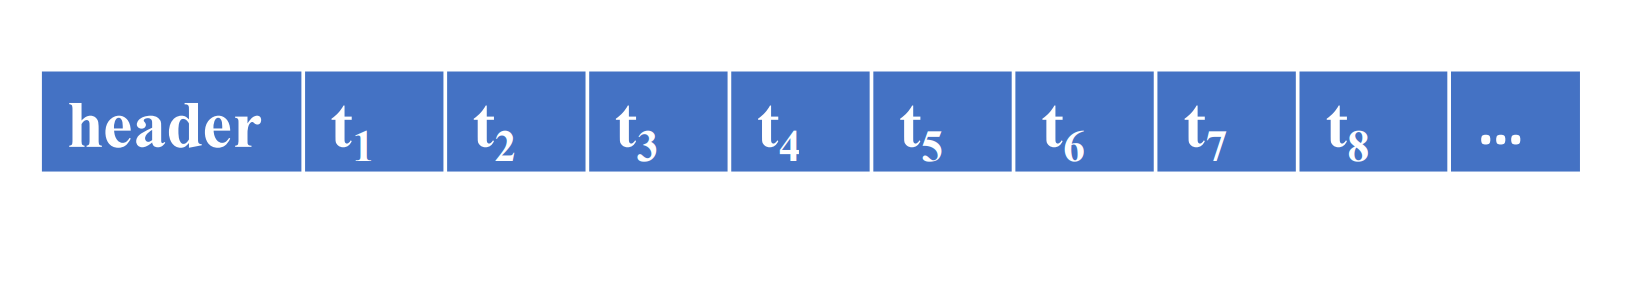
\includegraphics[width=0.9\linewidth]{figs/packetformat.PNG}
%     \caption{Estimation packet format}
%     \label{fig:estimation_packet_format}
% \end{figure}


% Notice that if the values of $x_{n}^{s}(t)$ and $y_{\ell}^{s}(t)$ are a feasible solution for the \myproblem problem, then $\sum_{n\in O_{t}} \delta_{n}(t)$ is the end-to-end delay. Next, we show how the system can collect the values of $\delta_{n}(t)$ (the delay incurred by using node $n$) in an efficient manner and send them back to the user. 

% In this section, we present our proposed Contextual combinatorial upper confidence bound algorithm (\cucb) for \myproblem. The basic idea of \cucb is to balancedly explore and exploit each arm in $\mc{A}$ by "adjusting" them before selecting. The algorithm performs as follow:

% During the learning slots, the algorithm will maintain: (1) variable $T_i$ as the total number of times arm $i$ is played so far; (2) variable $\hat{\mu}_i^t$ as the mean of all outcomes of arm $i$ observed so far, which will be used to adjust the estimation of each arm. 
% At each timeslot $t$, the algorithm first adjust each arm estimation and update the contextual information, which are then given to the oracle (denote as $\mc{O}$) as input.

% Then, the algorithm plays the super arm $S(t)$ returned by the oracle and uses the observed outcome to update $T_i$ and $\hat{\mu}_i^t$, while receiving an actual cost.
% The pseudo-code of the algorithm is summarized in algorithm \ref{alg:CMAB}.

% In step5, we apply an adjustment term to each arm estimation as follow:
% where $\hat{\mu}_i^t$ is the average estimate of arm $i$ so far at timeslot $t$,  $T_i$ is the number of times arm $i$ has been selected, by doing such adjustment we are performing what's called Upper Confidence Bound Selection\cite{UCB}, which uses uncertainty in the arm-value estimates for balancing exploration and exploitation, e.g. For those arms that have not been selected much times, its $T_i$ will be smaller and $\bar{\mu}_i^t$ will be smaller, this will increase the chance of arm $i$ being "explored". Moreover, $c$ decides the level of exploration, the bigger $c$ is, the more likely it is to explore a less selected arm, by doing this, we either gets the highest reward or we get to learn about an arm that we know least about.


%\subsubsection{Capacity measurement 1}
%Now we introduce two techniques for computing capacity and link capacity measurement respectively.
%For a reliable processing delay estimation on a computing node,  we apply $KOMon$ \cite{koMON} framework to measure the packet times of VNF through lightweight in-stack monitoring.

%For measuring link bandwidths along a path, we apply $pathchar$ \cite{jacobson1997pathchar}, $pathchar$ is a measurement tool developed by Van Jacobson at Lawrence Berkeley Laboratory (LBL), that can be used to find the bandwidth, delay, average queue and loss rate of every links in the network.

%$pathchar$ utilize the time-to-live (ttl) field of a IP packet, ttl  limits how many links it can traverse in the network before it expires, e.g. if a router receives an expired packet, it sends an ICMP error packet back to the sender, therefore the address of the $n$th router can be found by setting ttl to a value $n$. $pathchar$ works by sending probes with different ttl values and different sizes, it measures the time of each probes until the error packet returns, then it analyze the returned data based the following rtt formula from two nodes (say $n$ and $n-1$) using Van Jacobson's specifications:

%\begin{equation}
%\begin{aligned}
%   rtt &= q_1 + (latency + packet\_ size/bandwidth) + q_2 + forward \\   &   +q_3 + (latency + error\_size/bandwidth) + q_4,\\
%\end{aligned}
%\end{equation}

%where $q_i$ are random variables that represent the queuing delays between nth and n-1th node, $forward$ is the packet processing time when forwarding the packet. But $pathchar$ assumes three things: (1) the size of the error packet is negligible, (2) the forwarding time is negligible and (3) the queuing delays are negligible if enough measurements are made on a given path. Therefore we have:

%\begin{equation}
%   rtt = (latency + packet\_size/bandwidth) + latency.
%\end{equation}
%In our case, we apply the following probing steps on a SFC path to get the estimation of link latency and processing delay :
%\begin{enumerate}
%   \item At each timeslot, send multiple probe packets simultaneously to the $n$ nodes on the SFC path with various packet sizes, it then measures the round trip time (rtt) until a feedback packet is received, denoted by $rtt_n$
%  \item Each server i, upon receiving the probing packet, sends back a feedback packet with processing delay measured by KOMon(e.g. queue size), which will be used as processing capacity estimation. 
%   \item Analyze the feedback packet based on $pathchar$ and reconstruct link-by-link path characteristic
%\end{enumerate}
%A round trip time to node $n$ can for packet of size $s$ be expressed as
%\begin{equation}
%    rtt_n = \sum_{i=1}^n[s/b_i + d_i/c] + 2*\sum_{i=1}^n f_i
%\end{equation}
%A example for packet routing and probing in SFC placement is shown in figure 6.
% %\begin{figure}
%  %   \centering
%   %  \includegraphics[width=0.7\textwidth]{pathchar.PNG}
%     \caption{SFC packet routing and probing}
%     \label{fig:my_label}
% \end{figure}


% For analysis, we assume that the probing packet is small enough so that the processing delay and queuing delay can be negligible, therefore we have:
% \begin{equation}
%     rtt_n = 2*\sum_{i=1}^n f_i, n\in \mathcal{S}.
% \end{equation}

% \subsubsection{Capacity measurement 2}
% For processing delay measurement, using KoMON\cite{koMON}, for each computing node, upon receiving the first packet in a SFC request, it starts to calculate the processing delay and send it back to user after processing the last packet of SFC request. Processing delay piggy back packet will then be using the same timeslot as the SFC request. More specifically, the server doesn't have to know the exact timeslot, it just need to make sure that a task is finished and processing delay is calculated within a time interval, say $\tau$

% For processing delay, we apply SLAM\cite{SLAM} framework that is designed for SDN, SLAM is deployed on centralized controller and combines four components: rule generator, traffic generator, traffic listener, and latency estimator (as shown in Figure ). The latency computation process is composed of three steps: 
% \begin{enumerate}
%     \item  Preselect end-to-end path and install specific flow monitoring rules on all switches along the path. 
%     \item Controller sends constructed probe packets that match monitoring rules to switches and then the probe will traverse through the monitored path. Once the probe packet arrived at a switch, it will be regarded as a new flow and trigger Packet\_in message to controller. 
%     \item  Controller estimates path's latency based on the time-stamp in these messages. 
% \end{enumerate}


%currently 
% Now we introduce our $Capacity\ Update\ Protocol$ for measuring link capacity in one hop. it uses a simple timestamp insertion to the probing packet for the calculation of end-to-end delay from one computing node to another and the computing delay on a computing node. As depicted by Figure 6, each node inserts current time as a timestamp to the probing packet before sending it to the next node , while it also keeps track of time when processing the request. e.g., for a request with $\lambda^t$, Node A sends the request to Node B at $t_1$, Node B receives it at $t_2$ and finish the request at $t_3$, link capacity $LC$ and computing capacity $CC$ is then calculated by:
% \begin{equation}
%     LC = \lambda^t/(t_1-t_2),\  CC=\lambda^t/(t_3-t_2),
% \end{equation}
% In order to solve the issue that the system clocks of two edge nodes are usually not synchronized, we use $packet\ pair\ probing$\cite{1049160} that can give us a better estimation of link capacity. 
% Consider the scenario that Packet i arrives at link($A\rightarrow B$) at $\tau_i$ and leaves the link at $\tau^*_i$, the link delay is therefore 
% \begin{equation}
%     d_i = \tau^*_i - \tau_i = \lambda^i/LC, 
% \end{equation}
% We compare two adjacent packet we have:
% \begin{equation}
% \begin{aligned}
%     \text{inter-arrival time:}\ t_i&=\tau_i - \tau_{i-1}, \\
%     \text{inter-departure time:}\ t^*_i&=\tau^*_i - \tau^*_{i-1},\\
%     \text{delay variation:}\ \delta_i &= d_i - d_{i-1}=t^*_i-t_i\\
%     &=\lambda_i/LC - \lambda_{i-1}/LC\\
%     &=(\lambda_i-\lambda_{i-1})/LC.\\
%   \end{aligned}
% \end{equation}
% Therefore we have:
%     \begin{equation}
%         LC = (\lambda_i-\lambda_{i-1})/(t^*_i-t_i).
%     \end{equation}
% With packet pair probing we are able to calculate link capacity by using the interval between a packet pair that is not affected by the clock offset.

% For a more reliable processing delay estimation on a computing node,  we apply $KOMon$ \cite{8854514} framework to measure the packet times of VNF through lightweight in-stack monitoring. 


% \begin{figure}
%     \centering
%     \includegraphics[width=0.7\textwidth]{timestamp.PNG}
%     \caption{Delay Update Protocol (DUP)}
%     \label{fig:my_label}
% \end{figure}


% \subsection{Message Complexity Analysis}
% In our proposed framework we use the commonly deployed Transmission Control Protocol (TCP) as a measurement service. We now analyze the complexity of estimation packet.
% %In order to support the need for $KOMon$, we assume that all the computing nodes has KOMon module loaded into its kernel beforehand.  

% \subsubsection{Packet size}
% As we described before in packet format, each estimation packet requires $(l+1)*18$ bytes for storing information time stamps for a SFC of length $l$. Therefore a TCP based packet size will be:
% \begin{equation}
% \label{eqn: packet size cal}
%     20 + (l+1)*18 = 38+18l
% \end{equation}
% bytes in total with 20 bytes for the TCP header. As it may be concerned, here we do not consider the issue of clock synchronization\cite{clocksyn} due to the fact that all of our emulation experiments will be executed on virtual computing machines that are in the same time system. 

% \subsubsection{Number of packets sent in each timeslot}
% As it may be apparent, assume that $n$ packets are sent to measure each link bandwidth on a SFC, the number of packets sent in total can be calculated by:
% \begin{equation}
%     N = 1 + n*s,
% % \end{equation}
% where $s$ is the number of links on a SFC path.




% Explain how many packets (how many bytes) will be sent to collect estimated information. 

% TCP/IP header overhead discussion. 
% You are designing the body of the messages. 
% But, you use TCP/IP (or even UDP) to send them. 

% How many request packets will be sent in a single timeslot?
% How many response packets will be sent in a single timeslot?

% Processing delay measurement is easy.
% ** IMPORTANT **
% "How to measure link delays?"
% Link delay measurement
% Link delay monitoring
% Per-link delay estimation


%To mitigate the measurement uncertainty and obtain a robust placement that is able to handle system dynamics we design our algorithm based on the contextual combinatorial bandit problem. 


%  Where $C()$ and $P()$ is the combination and permutation function respectively. 

% At the beginning of the arm selection, only the user side information is known, such as user's location and user's request, which are used as the context information. The information about the nodes are unknown, but as learning slots proceeding and arms being chosen, the system may gain a better knowledge of the arms and make better decisions based on it. 

% The selection is made in a way that is shown in Figure \ref{fig: selectionmakingdiagram}. In each timeslot the user selects the same number of computing nodes that equals to the services as an arm to deploy the SFC, and then they send their traffic towards SFC and waiting for the task to be processed. Due to the mobility, the users may or may not change the nodes to place each service on.
% \begin{figure}
%     \centering
%     \includegraphics[width=0.9\linewidth]{system.PNG}
%     \caption{Selection making during two timeslots}
%     \label{fig: selectionmakingdiagram}
% \end{figure}
% % ========== END examples

% Based on the descriptions above, We now transform the SFC problem into a general Contextual CMAB. To better formulate the SFC placement into a multi-arm bandit problem, we first characterize each computation node $i$ using a feature vector $\mu$ and then the super arm set $\eta$ will be formulated based on the node feature vector and the service number in SFC, which has size $n$ calculated in (7). 

% \begin{equation}
% \begin{array}
%     % &\mu_i^t = [1/c^t_i, f^t_{i, 1}, ..., f^t_{i, n}],\\
%     &\eta = \{\eta_1, \eta_2, ..., \eta_N\},\\
%     &\eta^t = [\mu_1^t, ..., \mu_s^t].\\
%   \end{array}
% \end{equation}
% where $\eta^t$ is the arm set that is selected at timeslot $t$ and $\mu_s^t$ denotes the node that runs service $s$ at timeslot $t$.

%  \begin{algorithm}
% \caption{Contextual MAB}
% \begin{algorithmic}[1]
%  \renewcommand{\algorithmicrequire}{\textbf{Initialization:}}
%  \renewcommand{\algorithmicensure}{\textbf{Online Learning}}
%  \REQUIRE \ 
%   \STATE Initialize the cumulative context of each super arm $\eta_i$ in set $\eta = \{\eta_1, \eta_2, ..., \eta_n\}$, $B_i = \textbf{I}$ ($s*(2M+3)$ dimensional identity matrix), the estimated vector of each super arm: $\hat{\eta_i} = \textbf{0}$ ($s*(2M+3)$ dimensional zero vector), cumulative SFC cost of super arm $\eta_i$: $f_{\eta_i} = \textbf{0}$ 
%  \ENSURE  \
%   \FOR{each timeslot $t = 1,2,...,T$}
%   \STATE  \textbf{Sample} the aggregated cost $\theta_{\eta_i}(t)$ for each super arm $\eta_i$ from the posterior distribution $\mathcal{N}(b(t)^{\top}\hat{\eta_i}, v^2b(t)^{\top}B_{\eta_i}^{-1}b(t))$
%   \STATE \textbf{Select} the super arm $s(t) = argmin\theta_a(t)$ and receive an actual cost $r_t$
%   \STATE \textbf{Update} $B_{s(t)} = B_{s(t)} + b(t)b(t)^{\top}, f_{s(t)} = f_{s(t)} + b(t)r_t, \hat{\eta_s} = B^{-1}_{s(t)}f_{s(t)}$
%   \ENDFOR
%  %\RETURN $P$ 
% \end{algorithmic} 
% \end{algorithm}

%  Where $\lambda^t$ indicates the current SFC demand, $g^t$ indicates the current user location and $f^t$ records the last SFC placement. 

%  $v$ is a control parameter in algorithm 1.


% In this subsection we present how to transform the SFC placement problem in to a general contextual CMAB problem.


% For a network with $m$ nodes, We define the links as an arm set $\mathcal{L} = \{\ell_1^t, \ell_2^t, ...., \ell^t_m \}$, where $\elll_i^t$ represent the link set from node $i$, thus we have:
% \begin{equation}
%      \mathcal{L} = \{\ell_1^t, \ell_2^t, ...., \ell^t_m \}, \ \
%      l^t_i = \{f^t_{i,1}, f^t_{i,2}, f^t_{i,3}, ..., f^t_{i,m}\},
% \end{equation}


% where $f^t_{i,j}$ denotes the link attribute from node $i$ to node $j$ at timeslot $t$ (e.g. transmission delay). We then define the link arm set as a binary vector $X^t = [x^t_{1,2},...,x^t_{1,m},x^t_{2,1},...,x^t_{2,m}, ..., x^t_{m,1}, ..., x^t_{m,m}]$ for selection, where $x^t_i = 1$ means link arm $i$ is chosen.
% Computing nodes are defined as a arm set $\mathcal{N} = \{ c_1^t, c_2^t, ..., c_m^t\}$, where $c_m^t$ represents the computing capacity on node $n$. Again we define the node arm set as a binary vector $Y^t = [y_1^t, ..., y^t_m]$ for selection, where $y^t_i = 1$ means node arm $i$ is chosen. 


% Estimation of the single arms and collecting those estimations at the user-side for further placement decisions is explained in detail in section~\ref{section:estimation}. 


% \subsection{Arms formulation in \myproblem}
% The arms in our problem are a collection of links and nodes, that is, $\mc{A} = \mc{N}\cup\mc{L}$, where $\mc{N}$ denotes the set of all node arms, $\mc{L}$ denotes the set of all link arms and we use $\mc{A}$ to denote the set of all arms.
% We then further transform both link arms and node arms into aforementioned binary vector for section, denoted by $X^t$ and $Y^t$, therefore we can express the arm formulation for \myproblem as follow:
% \begin{equation}
%     \begin{aligned}
%       X^t &= \{x^s_n(t)\}.\qquad \forall n\in\mc{N}, s\in \mc{S}, t\in\mc{T}\\
%       Y^t &= \{y^s_\ell(t)\}.\qquad \forall \ell\in\mc{L}, s \in \mc{S}, t\in\mc{T}\\
%     \end{aligned}
% \end{equation}
% At each timeslot, the user need to decide a set of arm to deploy the current SFC, we denote it by $\mc{S}(t)$, the super arm consist of the node and link arms selected to place this SFC. Formally, the super arm can be expressed as:
% \begin{equation}
%     \begin{aligned}
%       & S_t  = \{x^s_n(t), y^s_\ell(t)\}_{s\in\mc{S}(t)}

%     \end{aligned}
% \end{equation}
% where
% \begin{equation}
%     \begin{aligned}
%       &  \sum_{n\in\mc{N}} x_{n}^{s}(t)  = 1. 
%     \qquad 
%     \forall s\in\mc{S}, t\in\mc{T}\\
%     &\sum_{s\in\mc{S}} x_{n}^{s}(t) \le 1. 
%     \qquad 
%     \forall n\in\mc{N}, t\in\mc{T}\\
%     \end{aligned}
% \end{equation}


% Similar to many existing works \cite{MABserviceplacement, Mobility-Aware},
% Specifically, computing delay is calculated from arm set $X$ while migration and transmission delay is calculated from arm set $Y$. Therefore we define the reward function at each timeslot to be:
% where $d^t_{cp}$, $d^t_{cm}$ and $s^t$ are the computing delay communication delay and switching cost respectively. Specially, our switching cost will be calculated from a general model that is based on link capacity and the size of the VNF that needs to be migrated, we have:
% \begin{equation}
%     s_{i,j}^t = \alpha \cdot  \lambda_{S_i}^t /f_{i,j}^t,
% \end{equation}
% where $\alpha$ is an adjustment coefficient, $\lambda_{S_i}$ represents the size of the VNF that provides service $S_i$. 
% \subsection{Reward function of a super arm}
% We define our reward function to be the objective of \myproblem, that is, the end-to-end delay perceived by user, which is mainly consist of three parts as formulated in section \ref{section: formulation}: computing delay, transmission and propagation delay, migration delay. 
% As defined before, the reward function of a super arm $S$ at timeslot $t$ can be expressed as:
% \begin{equation}
%     \begin{aligned}
%          r(S_t) &= \text{Min. } \sum_{i=1}^{4} \gamma_{i}\Gamma_{i}(t)
%     \end{aligned}
% \end{equation}


%
% To consider user's specific context such as mobility and requests, we define the current-time-slot information such as user's connected base station $\beta(t)$, SFC request $\Lambda(t)$ and previously selected super arm $S_{t-1}$ as the contextual information, denoted by $\mc{C}(t)$, which is expressed by:
% \begin{gather}
%     \mc{C}(t) = [\beta(t), \Lambda(t), S_{t-1}], \\
%     \Lambda(t) = [\lambda_{s_1}(t), ..., \lambda_{s_k}(t)], \\
%     S_{t-1} = \{x^s_n(t-1), y^s_\ell(t-1)\}_{s\in\mc{S}(t-1)}.
% \end{gather}


%
% In order to treat each arm individually and be able to use their information that can be observed when playing a super arm for further selection, we formulation each link and node as individual arms. More specifically, we assume that we are able to get an estimation of each link and node by time-stamp techniques that are introduced in section~\ref{section:estimation}.
% %
% We then define the super arm selection policy that constraints the combination of links and arms to be physically feasible in a network, and the context information used for selection. 

% \subsection{Arms formulation in \myproblem}
% We then further transform both link arms and node arms into aforementioned binary vector for section, denoted by $X^t$ and $Y^t$, therefore we can express the arm formulation for \myproblem as follow:
% \begin{equation}
%     \begin{aligned}
%       X^t &= \{x^s_n(t)\}.\qquad \forall n\in\mc{N}, s\in \mc{S}, t\in\mc{T}\\
%       Y^t &= \{y^s_\ell(t)\}.\qquad \forall \ell\in\mc{L}, s \in \mc{S}, t\in\mc{T}\\
%     \end{aligned}
% \end{equation}
% At each timeslot, the user need to decide a set of arm to deploy the current SFC, we denote it by $\mc{S}(t)$, the super arm consist of the node and link arms selected to place this SFC. Formally, the super arm can be expressed as:
% \begin{equation}
%     \begin{aligned}
%       & S_t  = \{x^s_n(t), y^s_\ell(t)\}_{s\in\mc{S}(t)}

%     \end{aligned}
% \end{equation}
% where
% \begin{equation}
%     \begin{aligned}
%       &  \sum_{n\in\mc{N}} x_{n}^{s}(t)  = 1. 
%     \qquad 
%     \forall s\in\mc{S}, t\in\mc{T}\\
%     &\sum_{s\in\mc{S}} x_{n}^{s}(t) \le 1. 
%     \qquad 
%     \forall n\in\mc{N}, t\in\mc{T}\\
%     \end{aligned}
% \end{equation}


% \subsection{Policy for choosing a Super arm}
%  To satisfy the requirements of a SFC when choosing a super arm, we use the routing constraint and link constraint introduced in section \ref{section: formulation} as the policy of choosing super arms:

% \begin{equation}
% \label{eqn: superarmpolicy}
% \begin{aligned}
%   & \sum_{\ell\in\delta^{+}(r)} y_{\ell}^{s_{i}}(t)
%     - \sum_{\ell\in\delta^{-}(r)} y_{\ell}^{s_{i}}(t)
%     = x_{n_r}^{s_{i}}(t) - x_{n_r}^{s_{i+1}}(t).\\
%     &\qquad\qquad\qquad\qquad\qquad\qquad\qquad\forall r \in\mc{R}^{'},t\in\mc{T}\\
%     &\sum_{s_{i}\in\mc{S}} \lambda_{s_{i+1}}(t)y_{\ell}^{s_{i}}(t) \le b_{\ell}(t).
%       \qquad\forall \ell\in\mc{L}, t\in\mc{T}\\
% \end{aligned}
% \end{equation}
%  We assume that the SFC path always starts from user's current connected station and goes back to it, as shown in Figure 2.
% % \begin{equation}
% % \label{eqn: superarmpolicy}
% %     \begin{aligned}
% %     & \sum^{m}_{i=1}\sum^{m}_{j=1}x_{i,j}^t = \sum^m_{i=1}y_i^t, x_i^t \in X^t, y_i^t \in Y^t, \\
% %     & S^t = [c^t_g, f^t_{i,j}, c^t_j, f^t_{j,p}, c^t_p, ..., f^t_g], \\
% %     &\sum^m_{j=1}x_{i,j}^t=1, \sum^m_{j=1}x_{j,i}^t=1,  c_i^t \in \mathcal{N}.\\
% %     \end{aligned}
% % \end{equation}
% % where the first equation constraints the number of selected nodes should equal the number of selected links due to the SFC-to-user loop, the second equation requires that the selected nodes and links are able to form a path that returns to user, the third equation constraints that for any node selected for super arm, only one incoming and ongoing link arm will be selected. 
% This policy will be applied in the Oracle of the placement algorithm introduced in the next section.


% \begin{algorithm}
% \setAlgoLined
% \caption{\cucb}
% \label{alg:CMAB}
% \begin{algorithmic}[1]
%  \renewcommand{\algorithmicrequire}{\textbf{Initialization:}}
%  \renewcommand{\algorithmicensure}{\textbf{Online Learning}}
%  \REQUIRE \ 
%   \STATE For $i \in \mc{A}$ , maintain: (1)variable $T_i$ as the total number of times arm $i$ is played so far; (2) variable $\hat{\mu}_i^t$ as the mean of all outcomes of arm $i$ observed so far.
%   \STATE For each arm $i \in \mc{A}$, get a initial estimation $\hat{\mu}_i^0$ and set $T_i$ to 1.   
%   \STATE Initialize contextual $\mc{C}(1) = [\beta(1), \Lambda(1), S_0]$
%  \ENSURE  \
%   \FOR{$t \leftarrow 1,2,...,T$}
%     \FOR {$i \in \mc{A}$}
%     \STATE$\bar{\mu}_i^t \leftarrow \hat{\mu}_i^t - \sqrt{ \frac{3\ln t}{2T_i}}$.
%     \ENDFOR
%   \STATE $\mc{C}(t)\leftarrow [\beta(t), \Lambda(t), S_{t-1}]$
%   \STATE $S_t \leftarrow \mc{O}(\mc{C}(t), \{\bar{\mu}_1^t\}_{i\in\mc{A}}) $.
%   \STATE Select super arm $S_t$ and observe $\{\mu_i^t\}_{i\in{S_t}}$
%   \STATE Receive an actual cost $r(S_t)$
%   \STATE Update all $T_i$'s and $\hat{\mu}_i^t$'s, 

%   \ENDFOR
%  %\RETURN $P$ 
% \end{algorithmic} 
% \end{algorithm}


%  \begin{algorithm}
% \caption{DP-based oracle}
% \label{alg: oracleDP}
% \begin{algorithmic}[1]
%  \renewcommand{\algorithmicrequire}{\textbf{Input:}}
%  \renewcommand{\algorithmicreturn}{\textbf{Output:}}
%  \renewcommand{\algorithmicensure}{\textbf{Oracle:}}
%  \REQUIRE \ 
%   \STATE Adjusted arm estimation $\{\bar{\mu}_i^t\}_{i\in\mc{A}}$.
%   \STATE Context $\mc{C}(t) \leftarrow [\beta(t), \Lambda(t), S_{t-1}]$,
%  \ENSURE  \
%  \STATE Initialize $H(i,j) \leftarrow \mathbf{0};\quad \forall i\in \mc{S}[t], \forall
%  j\in \mc{N} $
%  \STATE Initialize $\text{Cost}(i,j)\leftarrow 0;\quad \forall i\in \mc{S}[t], \forall
%  j\in \mc{N}$
%   \FOR{$i = | \Lambda(t)|\to 0$}

%   \FOR{$j \in \mc{N} $}

%         \STATE  Compute and update $\text{Cost}(i,j), k$ according to eq.22-24
%         \STATE $H(i,j) \leftarrow H(i-1, k).append(k)$ 

%   \ENDFOR

%   \ENDFOR
%   \STATE Extract the node with the minimum cost to place vnf 1: $n \leftarrow \text{argmin}\{\text{Cost}(1, j)\}_{j \in \mathcal{N}}$

%   \STATE Get the corresponding host list as the super arm $S_t \leftarrow H(1, n)$
%  %\RETURN $P$ 
%  \RETURN Super arm $S_t$


% \end{algorithmic} 
% \end{algorithm}
%  \subsection{Time complexity}
%  The dynamic approach described in the oracle above is summarized in algorithm \ref{alg: oracleDP}, which results in a time complexity of $O(sn^2)$  with $n$ nodes and $s$ services, that is a bearable algorithmic time.


%All delays above can be calculated from the input arm estimation, .
%  In our CMAB algorithm, the oracle we used is a geo-ranged $argmin$ function (with $\alpha=\beta=1$) that is shown in Algorithm 3.

%  \begin{algorithm}
% \caption{SFC placement oracle}
% \begin{algorithmic}[1]
%  \renewcommand{\algorithmicrequire}{\textbf{Input:}}
%  \renewcommand{\algorithmicensure}{\textbf{Oracle}}
%  \REQUIRE \ 
%   \STATE Arm estimation vector $\hat{\mu} = [\bar{\mu}_1^t, \bar{\mu}_2^t, ..., \bar{\mu_m}^t]$.
%   \STATE Context vector $b(t) = [\lambda^t, g^t, F^{t-1}]$,
%   \STATE Current round time $t$, 
%   \STATE Selection range $r$.
%  \ENSURE  \
%   \FOR{each computing node $n$ within $r$ distance from $g^t$}
%   \STATE add it to the candidate list $C$
%   \ENDFOR
%   \STATE \textbf{LIST} all the subsets with the size equals to $\lambda^t$ from $C$

%   \STATE \textbf{COMPUTE} the cost $Cost_s(t)$ each subset $s$ in $C$, and set the subset with the least cost as the super arm.
%  %\RETURN $P$ 
% \end{algorithmic} 
% \end{algorithm}


% \begin{figure}
%     \centering
%     \includegraphics[width=0.9\linewidth]{oracle.PNG}
%     \caption{Oracle in SFC placement}
%     \label{fig:oracle}
% \end{figure}

% In SFC placement, the oracle limits that the selected nodes and links are able to be connected and formed into a complete SFC path. The selection of the exact optimal SFC path can be computationally hard and the learning algorithm may have a small failure probability. Thus, we resolve to the following $(\alpha,\beta)$-approximation oracle\cite{chen2013combinatorial}: For some $\alpha, \beta \leq 1$ that takes an expectation vector \texbf{$\mu$} as input, and outputs a super arm S such that :
%  \begin{equation}
%      Pr[r_{\mu}(S) \geq \alpha \cdot r_{\mu}(S_{opt})]\geq\beta
%  \end{equation}
%  Here $r_{\mu}()$ is the reward function, $S_{opt}$ is the exact optimal super arm and $\beta$ is the success probability of the oracle.


% $Oracle$ in the algorithm works as a super arm selection policy, it takes the estimates of individual arms as input and output a super arm for placement, as already mentioned before, it will follow the constraints in (11) when generating an super arm. More specifically, it explore all the nodes within a certain distance from user's current location and calculate the optimal combination of individual arms in terms of service cost based on the estimation.
% Contextual information $b(t)$ is also required in our algorithm and is formulated as (11). 


%
% \subsection{Related work}
% Probing techniques have been well study in the literature, we introduce two approaches: \cite{article, alizadeh2014conga} propose two different method of probe in order to get the link information, and use them in routing and load balancing respectively.
%
% In \cite{alizadeh2014conga}, the author present Conga, which focuses on the measurement of a link load, the idea of this method to measure a link between two nodes is to send packets and create a feedback loop between the sender and receiver to populate the metrics through the link. To store and estimate the metrics, they use DRE (discounted rate estimator), which maintains a register $X$, that is incremented for each packet sent over the link by the packet size in bytes, and is decremented periodically with a multiplicative factor $\alpha$ between 0 and 1: $X = X\times(1-\alpha)$. 
% the metric that needs to be measured in their case is congestion between two nodes.
%
% HyMAB \cite{article}
% on the other hand, focus on the strategy of finding a optimal multipath for a single flow in routing problem in order to get an optimal throughput. They proposed algorithm HyMAB, which treats each multi-path as arms, each time they choose one multipath to probe and get a reward. the arm is chosen based on a multi-arm bandit strategy that are introduced in \cite{auer2002finite}.
%
% After a arm is chosen which means the multipath is given, they compute an optimal rate on this path by solving a max rate linear problem.
% Now we present our time-stamp based estimation framework in SFC placement to measure the processing delays on each computing node and the transmission delay on each link. %Estimation of these two metrics will be stored in a SFC capacity vector (denoted by $E$) that returns to user along with the SFC response.


% Depending on the length of SFC, say $l$, each estimation packet would occupy $(l+1)*18$ bytes of payload to store all the time stamps because each time stamps takes 18 bytes to store in our implementation.
% \begin{itemize}
%     % \item \textbf{$nid_i (2 bytes)$}: this field is used by the nodes along the path to store the node id of the $i$th node in the SFC.
%     \item \texbf{$\Lambda_i(4bytes)$} : this field is used to store the size of SFC packets
%     \item \textbf{$t_i(4bytes)$}: link capacity, this field is used to store the time stamp.
%     % \item \textbf{DT}: Delay Table, This is a M-M table that stores the transmission delays in the networks at timeslot t, specifically for a node i, $T^t_i = [g^t_{i,1}, g^t_{i, 2}, ..., g^t_{i, M}]$, this table will be maintained by destination node based on index: SN and DN, one transmission delay metric will be inserted in this table after destination node receive the probe packet and calculate a delay.    
% \end{itemize}


% We apply an adjustment term to values obtained from above to encouraging exploring for the future rounds. For each link delay and computing delay we estimate from a SFC response, we can record the times of the same element that has been updated, for element $i$, we denote the total number of times it's been updated as $T_$ and apply the following adjustment:
% \begin{equation}
% \label{eqn:adjustment}
%     \bar{\mu_i} = \hat{\mu_i} - e * \sqrt{ \frac{3\ln t}{2T_i}},
% \end{equation}
% where $t$ is the current round number, $e$ is a configurable constant.


% \subsection{Oracle}
% \label{section: oracle}


%\section{Estimation of single arms}


% \subsubsection{Delay feedback}
% We use a feedback loop between the source node and the destination node for us to gain estimations for Computing capacity vector and transmission delay table. The probing process is described as follow:
% \begin{enumerate}
%     \item The source node first sends the probe packet to MEC network with the $nid_1$ field set to its node id and $c_i$ set to its computing capacity. 
%     \item As the packet routing through the MEC, each nodes it passes will calculate the link capacity from the last node before it process the packets and add it to f field, it also calculates it own computing capacity and insert it into $C^t$ vector in CC field.
%     \item When the packet is received at the destination node, it will add its transmission delay from last node to the TD field which will be the delay estimation from source node to destination node. Then it will add its computing capacity to the CC field and prepare for piggyback.
%     \item when a packet is sent in the reverse direction, the aggregated delay metric will be inserted to the delay table based on the source node id in SN field and destination node id.
%     \item Finally, the source node received and parse the piggyback packet and get a partial estimation of capacity vector and delay table.
% \end{enumerate}
%\subsection{SFC feedback}
%\subsubsection{SFC-to-user feedback loop}
%In our user-based SFC problem, we use a SFC-to-user feedback loop to obtain the network information. Explicitly we assume that probing process is within the SFC process, that is, when the SFC request is roaming through the VNFs (virtual network functions), the estimation packet will also be passed on the nodes that has the VNFs placed on along with the SFC packets. In the end of a timeslot, the user will not only receive a SFC response but also an updated estimation vector, this process is illustrated in figure 5.
%\begin{figure}
%    \centering
%   \includegraphics[width=0.7\textwidth]{probingservicechain.PNG}
%  \caption{Probing in SFC placement}
% \label{fig:my_label}
%\end{figure}


% Especially for processing delay, the error might be amplified by the size of the processing packet.


% The basic steps of DP can be summarized as follow:
% \begin{itemize}
%     \item characterizing the structure of an optimal solution
%     \item Defining the cost of an optimal solution recursively
%     \item Computing the cost of an optimal solution in a bottom-up fashion
% \end{itemize}


% \begin{equation}
%      \bar{\mu}_i^t = \hat{\mu}_i^t - c* \sqrt{ \frac{3\ln t}{2T_i}}, 
% \end{equation}


% However, the formulation in general CMAB yields an exponential number of arms as shown in equation \ref{eqn:number of super arms}, which may have computational limitations and this approach of forming super arms will also neglect the information of single arms that can be observed from the outcomes received after choosing a super arm.


% \theta_{n} = [\frac{1}{c_{n}}(t), \rho_{a,b}^{s}(t)]^{\intercal} \\
% \chi_{n}^{s_i}(t) = [\pi_{s}\lambda_{s}(t), x_{b}^{s}(t-1)]^{\intercal} \\
% \theta = [\theta_{n}]^{\intercal} \\
% \chi_{n}(t) = [\chi_{n}^{s_1}(t),\dots,\chi_{n}^{s_S}(t)] \\


% Note that the propagation delay of a link is a function of distance and does not depend on the location of the user or the placement of the services. Thus, for each link $\ell$ the delay $\delta_{\ell}(t)$ is simply defined as,
% \begin{gather}
%     \delta_{\ell}(t) = d_{\ell}(t) + \epsilon_{n}(t).
% \end{gather}


% In this section we present our proposed CMAB formulation for \myproblem and then we introduce a contextual combinatorial upper confidence bound ($\text{C}^2\text{UCB}$) algorithm with a Dynamic Program (DP) based oracle that solves the CMAB problem.


% \begin{algorithm}[t]
%     \DontPrintSemicolon
%     \caption{RL-based chain allocation}
%     \label{alg:CMAB}
%     \SetKwInput{kwInit}{Init}
%     \KwIn {$\lambda$, $\{\pmb{\chi}_{n}(0)\}$}
%     \kwInit{}
%     \For{$t \in \mc{T}$}{
%         \For{$n \in \mc{N}$}{

%         }
%         $O_{t} \gets$ get\_alloc($\{\hat{\delta}_{n}(t)\}$, $\{\pmb{\chi}_{n}(0)\}$)
%         \hfill //See Alg. \ref{alg:get_alloc} \\

%     }
% \end{algorithm}


% In the following, we explain the definition of feature vectors and the approach of selecting appropriate set of servers and links for the placement of the service chain in each timeslot.


% To collect these information, we design a lightweight timestamp-based delay estimation and distribution framework to lower the overhead and facilitate deployability. 
% %
% To estimate delays in the network, {\color{red} This sentence is a bit vague, we should discuss it more: we time-stamp one packet and tag it along with the packets that we send for each SFC request while keeping track of the time.} The estimation framework has two parts:
% \begin{itemize}[leftmargin=*]
%     \item \textbf{An initial estimation of the whole network:} {\color{red} I think we can make this part more sophisticated... for example define a radius of servers that we recieve an estimation for them.} The user first sends a request to each computing node, upon receiving the request, the server will send packets to the other servers and time stamp them. After receiving all the returned packets, the server parse the time stamps in them, calculate the delays and send those information back to the user. The user collect all the delay estimations from the servers and save it as a initial estimation that is required in the CMAB algorithm.
%     \item \textbf{Estimation of delays on the chosen SFC path:} We also time-stamp the packets we send in each SFC request, after the packet is returned from the SFC, the user parses the time stamps and calculates the delays on the SFC. Those estimations will then be used to update the initial estimation in accordance with algorithm \ref{alg:CMAB}.
% \end{itemize}


% \cat{Example 2}
% Consider a SFC with three different services as an example. The formatting of the packet that's used for estimation is shown in figure \ref{fig:estimation_packet_format}, each server on the path append the time stamps to the packet during the service. 
% We consider a scenario that the VNFs are placed on node A, B, C at the moment and that user is connected to node D, as shown in figure \ref{fig:timestampsMEC}. The SFC request from a mobile user will be time stamped and recorded, as the request being handled on the chain, each processing node will time stamp the packet when it receives a packet and after the processing is done. The time-stamping process is described as follow:
% \begin{enumerate}[leftmargin=*]
%     \item  User generates SFC request packets with size $\lambda_i$ bytes for each service $i$, while inserting the current time to $t_1$ to the last packet.
%     \item Node A receives the request first in the SFC, upon receiving the last packet, it update the packet by inserting its current time $t_2$ and start processing the packets. When the processing is done, node A insert the current time $t_3$ to the same packet , then it sets the destination to node B as the next service handler and forward all the packets.
%     \item Node B process the second requested task and insert time stamp $t_4$, $t_5$ before and after the task respectively. Then it sets the destination to C and forward the packets.
%     \item Node C processes the last request, it repeat the time stamping ($t_6$, $t_7$) and send a SFC response along with a packet that stores all the time stamps in order.
%     \item Finally, the user receives the response for their services and a list of traversed time stamps while recording the current time $t_8$ upon receiving. 
% \end{enumerate}
% Based on the time stamps and SFC packet sizes, user are able to calculate the corresponding estimated link delay and processing delay as follow:
% \begin{equation}
%     \label{eqn:timestampcalculation}
%     \begin{aligned}
%     d_{D \rightarrow A} &= t_2 - t_1\\
%     d_{A \rightarrow B} &= t_4 - t_3\\
%     d_{B \rightarrow C} &= t_6 - t_5\\
%     d_{C \rightarrow D} &= t_8 - t_7\\
%     d_A           &= (t_3 - t_2)/\lambda_1\\
%     d_B           &= (t_5 - t_4)/\lambda_2\\
%     d_C           &= (t_7 - t_6)/\lambda_3\\
%     \end{aligned}
% \end{equation}

% \begin{figure}[t]
%     \centering
%     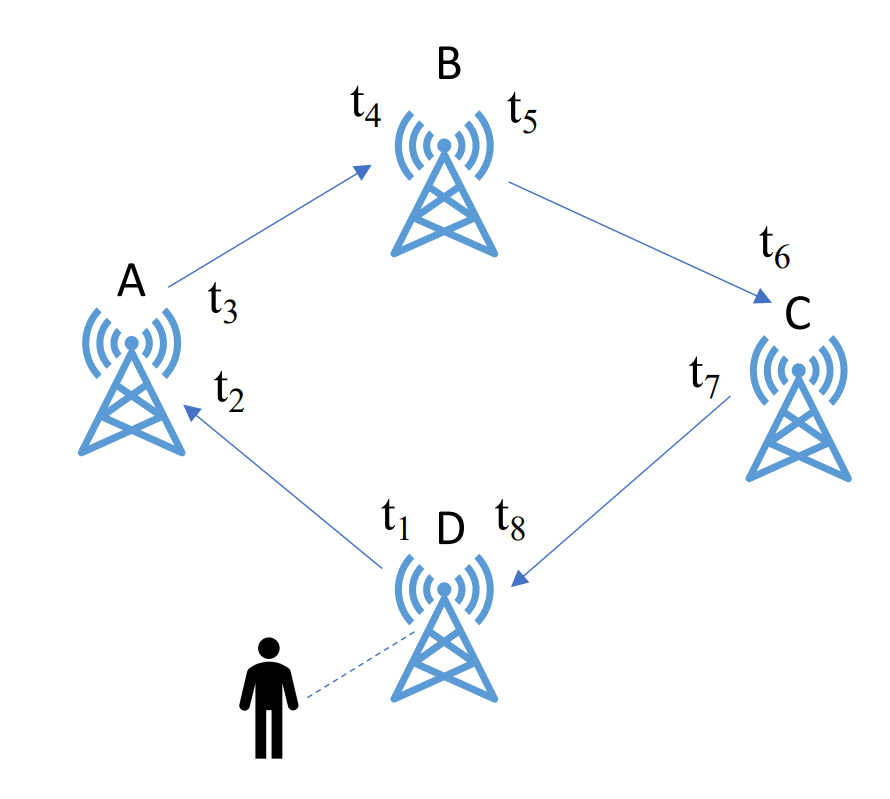
\includegraphics[width=0.9\linewidth]{figs/SFCtimestamp.PNG}
%     \caption{Time stamps of SFC placement in MEC}
%     \label{fig:timestampsMEC}
% \end{figure}


% We use the contextual combinatorial bandit framework to characterize the placement options that the user can choose from. This framework allows the user to employ the reinforcement learning and account for the relation between the perceived quality of service in terms of delay and the service type, traffic rate, and the mobility. Also,
\chapter{\textbf{Delay Estimation framework}}
\label{chap:estimation}
As already mentioned before, to decide on a solution (super arm), we need first to gain estimation for each individual's arms. In our problem, we assume that by selecting a super arm, we are able to get an estimation of every single arm in it (i.e: computing delay and link delay) and update the estimated values accordingly. 
In this chapter, we present our design of a time-stamped based estimation framework to measure the delay in the network, which we implement and apply for each Mininet-WiFi experiment conducted in chapter \ref{chapter: Mininet-wifi Experiments}. 

%\subsection{Related work}
%Probing techniques have been well studied in the literature. We introduce two approaches: \cite{article, alizadeh2014conga} propose two different methods of probing in order to get the link information and use them in routing and load balancing, respectively.
%
%In \cite{alizadeh2014conga}, the authors present Conga, which focuses on the measurement of a link load. The idea of this method to measure a link between two nodes is to send packets and create a feedback loop between the sender and receiver to populate the metrics through the link. To store and estimate the metrics, they use DRE (discounted rate estimator), which maintains a register $X$, that is incremented for each packet sent over the link by the packet size in bytes and is decremented periodically with a multiplicative factor $\alpha$ between 0 and 1: $X = X\times(1-\alpha)$. 
%The metric that needs to be measured in their case is congestion between two nodes.
%
%Authors in HyMAB \cite{article}
%on the other hand, focus on the strategy of finding optimal multi-path for a single flow in routing problem in order to get an optimal throughput. The proposed algorithm HyMAB, treats each multi-path as arms. Each time it chooses one multi-path to probe and get a reward. The arm is chosen based on a multi-arm bandit strategy that is introduced in \cite{auer2002finite}.
%
%After an arm is chosen, which means the multi-path is given, they compute an optimal rate on this path by solving a max rate linear problem.

\section{Time stamp in SFC placement}
Now we present our proposed time-stamp based estimation framework in SFC placement to measure the processing delays on each computing node and the transmission delay on each link. %Estimation of these two metrics will be stored in a SFC capacity vector (denoted by $E$) that returns to the user along with the SFC response.
To estimate the delays in the network, we time-stamp\cite{} one packet and tag it along with the packets we send for each SFC request while keeping track of the time. The estimation is consist of two parts:

1) \textbf{An initial estimation of the whole network.} The user first sends a request to each computing node. Upon receiving the request, the server will each send packets to the other servers and time stamp them. After receiving all the returned packets, the server parses the timestamps in them, calculates the delays, and sends that information back to the user. The user collects all the delay estimations from the servers and saves them as a initial estimation required in the CMAB algorithm.

2) \textbf{Estimation of delays on the nodes and links that have been selected for placeing SFCs.} Like the initial estimation, we also timestamp the packets we send in each SFC request. After the packet is returned from the SFC, the user parses the timestamps and calculate the delays on the SFC. Those estimations will then be used to update the initial estimation according to algorithm~\ref{alg:cccpa}.
We consider a SFC with three different services in this section as an example. The packet format of the packet that's used for estimation is shown in figure \ref{fig:estimation packet format}. Each server on the path appends the timestamps to the packet as the packet traverses. Depending on the length of SFC, say $l$, each estimation packet would occupy $(l+1)*18$ bytes of payload to store all the timestamps because each time stamps takes 18 bytes to store in our implementation.


% \begin{itemize}

%     % \item \textbf{$nid_i (2 bytes)$}: this field is used by the nodes along the path to store the node id of the $i$th node in the SFC.
%     \item \texbf{$\Lambda_i(4bytes)$} : this field is used to store the size of SFC packets
%     \item \textbf{$t_i(4bytes)$}: link capacity, this field is used to store the time stamp.

%     % \item \textbf{DT}: Delay Table, This is a M-M table that stores the transmission delays in the networks at time slot t, specifically for a node i, $T^t_i = [g^t_{i,1}, g^t_{i, 2}, ..., g^t_{i, M}]$, this table will be maintained by destination node based on index: SN and DN, one transmission delay metric will be inserted in this table after destination node receive the probe packet and calculate a delay.    

% \end{itemize}
\begin{figure}
	\centering
	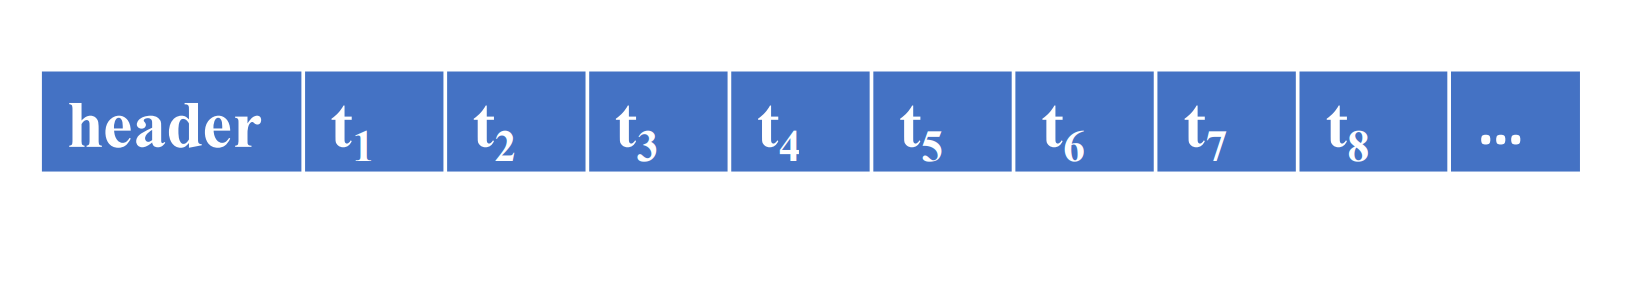
\includegraphics[width=0.9\linewidth]{figs/packetformat.PNG}
	\caption{Estimation packet format}
	\label{fig:estimation packet format}
\end{figure}
% \subsubsection{Delay feedback}
% We use a feedback loop between the source node and the destination node for us to gain estimations for Computing capacity vector and transmission delay table. The probing process is described as follow:
% \begin{enumerate}
%     \item The source node first sends the probe packet to MEC network with the $nid_1$ field set to its node id and $c_i$ set to its computing capacity. 
%     \item As the packet routing through the MEC, each nodes it passes will calculate the link capacity from the last node before it process the packets and add it to f field, it also calculates it own computing capacity and insert it into $C^t$ vector in CC field.
%     \item When the packet is received at the destination node, it will add its transmission delay from last node to the TD field which will be the delay estimation from source node to destination node. Then it will add its computing capacity to the CC field and prepare for piggyback.
%     \item when a packet is sent in the reverse direction, the aggregated delay metric will be inserted to the delay table based on the source node id in SN field and destination node id.
%     \item Finally, the source node received and parse the piggyback packet and get a partial estimation of capacity vector and delay table.
% \end{enumerate}

%\subsection{SFC feedback}
%\subsubsection{SFC-to-user feedback loop}
%In our user-based SFC problem, we use a SFC-to-user feedback loop to obtain the network information. Explicitly we assume that probing process is within the SFC process, that is, when the SFC request is roaming through the VNFs (virtual network functions), the estimation packet will also be passed on the nodes that has the VNFs placed on along with the SFC packets. In the end of a time slot, the user will not only receive a SFC response but also an updated estimation vector, this process is illustrated in figure 5.
%\begin{figure}
%    \centering
%   \includegraphics[width=0.7\textwidth]{probingservicechain.PNG}
%  \caption{Probing in SFC placement}
% \label{fig:my_label}
%\end{figure}
\section{Time-stamped delay estimation example}
We consider a scenario that the VNFs are placed on node A, B, C at the moment and that the user is connected to node D, as shown in figure~\ref{fig:timestampExample}. The SFC request from a mobile user will be time-stamped and saved as a vector as we defined before, as the request is handled along the chain, each processing node will time stamp the packet when: 1) When it receives a packet, 2) After it is done processing. The probing process is described as follow:

1) User generates SFC request packets with size $\lambda_i$ bytes for each service $i$, while inserting the current time to $t_1$ in the last packet.

2) Node A receives the request first in the SFC. Upon receiving the last packet, it updates the packet by inserting its current time to $t_2$ and starts processing the packets. When the processing is done, node A inserts the current time $t_3$ to the same packet. Then it sets the destination to node B as the next service handler and forwards all the packets.

3) Node B process the second requested task and inserts timestamps $t_4$, $t_5$ before and afterward the task, respectively. Then it sets the destination to C and forwards the packets.

4) Node C processes the last request. It repeats the time-stamping ($t_6$, $t_7$) and sends a SFC response along with a packet that stores all the timestamps in order.

5) the user will then get a response for their services and a list of timestamps while recording the current time $t_8$ upon receiving. Based on the timestamps and SFC packet sizes, the user is able to calculate the corresponding link delay and processing delay.

\begin{figure}
	\centering
	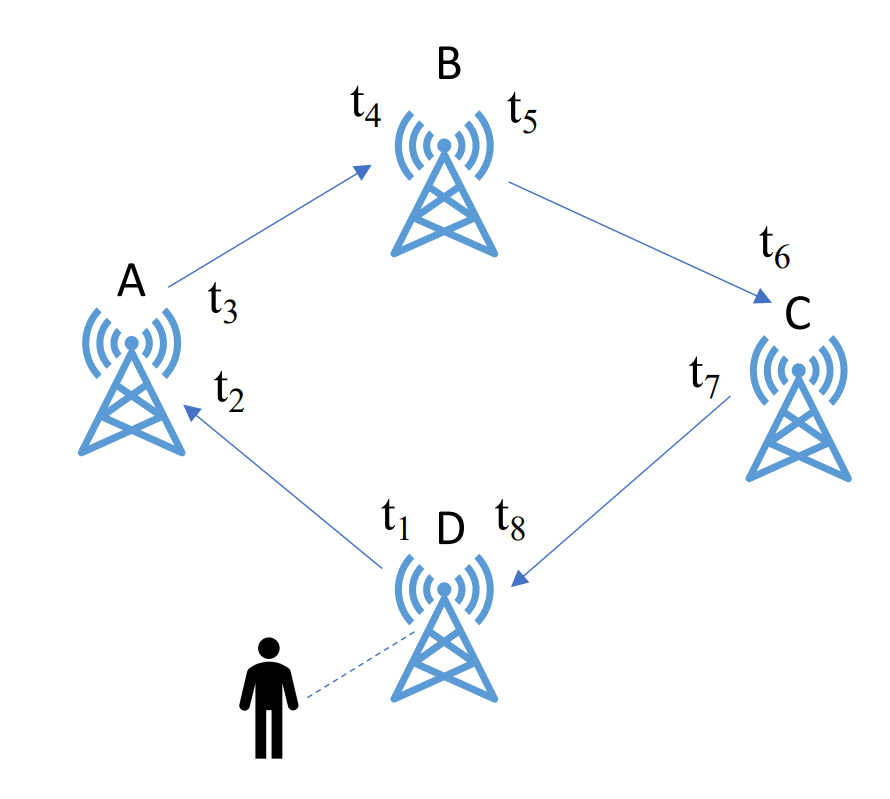
\includegraphics[width=0.9\linewidth]{figs/SFCtimestamp.PNG}
	\caption{Time stamps of SFC placement in MEC}
	\label{fig:timestampExample}
\end{figure}
When the time stamps is returned to user, they can analyze the packet and calculate the delays on the SFC path as follow:
\begin{equation}
	\label{eqn: timestampcalculation}
	\begin{aligned}
		LinkDelay_{D \rightarrow A} &= t_2 - t_1\\
		LinkDelay_{A \rightarrow B} &= t_4 - t_3\\
		LinkDelay_{B \rightarrow C} &= t_6 - t_5\\
		LinkDelay_{C \rightarrow D} &= t_8 - t_7\\
		ProcessingDelay_A           &= (t_3 - t_2)/\lambda_1\\
		ProcessingDelay_B           &= (t_5 - t_4)/\lambda_2\\
		ProcessingDelay_C           &= (t_7 - t_6)/\lambda_3\\
	\end{aligned}
\end{equation}

% We apply an adjustment term to values obtained from above to encouraging exploring for the future rounds. For each link delay and computing delay we estimate from a SFC response, we can record the times of the same element that has been updated, for element $i$, we denote the total number of times it's been updated as $T_$ and apply the following adjustment:
% \begin{equation}
% \label{eqn:adjustment}
%     \bar{\mu_i} = \hat{\mu_i} - e * \sqrt{ \frac{3\ln t}{2T_i}},
% \end{equation}
% where $t$ is the current round number, $e$ is a configurable constant.
\chapter{\textbf{Simulation Results}}
\label{chapter:simulation}
In this chapter, we conduct extensive simulations to demonstrate the performance of our proposed online learning algorithm \myalgorithm\ for user-managed SFC placement on edge, in terms of the convergence performance, scalability, and relative performance against other algorithms under varying parameters. All algorithms are implemented in Python 2.7 and run on an Intel Core i5-7400CPU@3.00GHz machine with 8.00 GB RAM. We utilize the Python interface of Networkx \cite{networkx} to simulate customized network and Gurobi \cite{gurobi} to solve the optimal offline optimizations.


% In this chapter, we evaluate our proposed algorithm. We first conduct a set of simulation experiments to show the performance of \myalgorithm under different environmental settings and scalability. Then we validate the algorithm in a \textit{Mininet-wifi} emulation by showing its performance under real environmental dynamics.
\section{Simulation Settings}
\begin{table}
	\centering
	\caption{Simulation parameters}
		\vspace{\baselineskip}
	\label{tab:Simulation parameters}
	% \resizebox{\columnwidth}{!}
	\begin{tabular}{ll}
		\toprule
		Parameter & Value \\[5pt]
		\midrule
		Number of nodes & 26 (25 edge, 1 cloud)\\[5pt]
		
		Edge VNF proc. delay (ms/kbit) & 0.5 - 1 (uniform)\\[5pt]
		Cloud VNF proc. delay (ms/kbit) & 0.1\\[5pt]
		Number of links & 65\\[5pt]
		Link delay (ms) on edge & 10 - 50 (uniform) \\[5pt]
		Link delay (ms) edge2cloud & 100 - 200 (uniform) \\[5pt]
		Migration delay (ms)& 10 - 200 (uniform)\\[5pt]
		VNFs per SFC requests &  3 - 5\\[5pt]
		VNF request (bits) & [250, 2500, 10000]\\[5pt]
		Mobility model & Random Waypoint \\ [5pt]
		
		\bottomrule
	\end{tabular}
\end{table}

\subsection{Network Settings}
We conduct experiments on a simulated 2km $\times$ 2km grid network area with 25 edge nodes and a cloud node, as shown in figure \ref{fig:simtopology}, this setting is in line with \cite{MABserviceplacement}. 
%
Cloud and each edge server is equipped with computation ability, 
The ratio of processing delay factors $\pi_s$ to node capacities is set appropriately to achieve a processing delay of [0.5, 1]  and  0.1 milliseconds per Kbits of data flow for each edge computing node and 0.1 milliseconds per Kbits of data flow for the cloud. 
%
The link delay of user-to-edge and edge-to-cloud links are uniformly distributed in [10, 50] milliseconds and [100, 200] milliseconds, respectively.  The migration delay is proportional to the link delays and thereby is distributed in [10, 200] milliseconds depending on the link that the VNF is migrated through.

%for each edge server, the processing delay is uniformly distributed in [0.5, 1] ms/kbit, and the processing delay on the cloud is 0.1 ms/kbit. The link delay on the edge is uniformly distributed in [10, 50] ms  and the link delay from each edge to cloud is uniformly distributed in [100, 200] ms. we assume that migration delay is proportional to link delay, therefore uniformly distributed in [10, 200] ms depends on the link that the VNF is migrated through. 
We set these values based on~\cite{SFCsettingsapp} so that the environment can provide the conventional end-to-end delays for existing applications (\eg\ web service $500$ms, video streaming $100$ms, and online gaming $60$ms). 

\begin{figure}
	\centering
	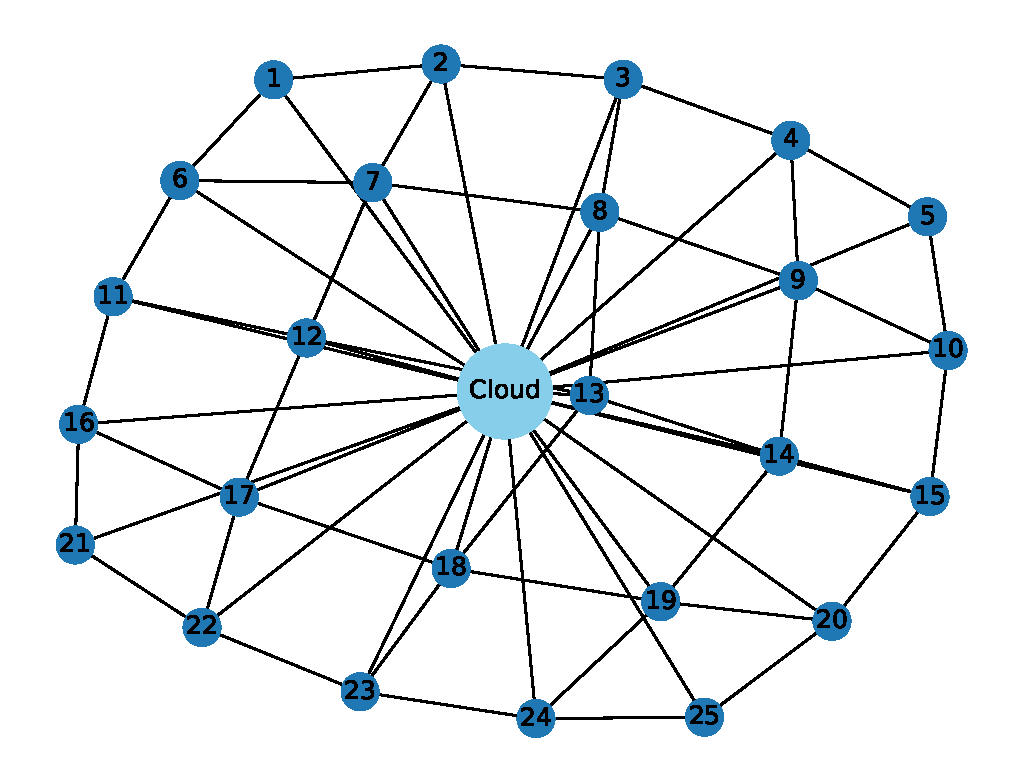
\includegraphics[width=0.9\textwidth]{figs/topology.eps}
		\vspace{\baselineskip}
	\caption{Network topology used in simulation}
	\label{fig:simtopology}
\end{figure}


% For  \textit{networkx}\cite{networkx}. On each node and each link, we add three attributes: actual weight, estimated weight and selected times.
%Actual weights on the nodes are uniformly distributed in  [10, 15] Gbps representing the computing capacity on each nodes, denoted by $c_i$, the capacity on the cloud are set to 100 Gbps. Actual weights on the link represents the
% transmission delay, denoted by $l_{i,j}$. The transmission delay between connected base station or AP is uniformly distributed in [50, 100] ms, the transmission delay to cloud node from each edge node are uniformly distributed in [100, 300] ms. Estimated weights are uniformly distributed in a range based on the actual weight with a noise $n$, that is, $\hat{c}_i^t \sim U(c_i-n, c_i+n)$ and $\hat{l}_{i,j}^t \sim U(l_{i,j} -n, l_{i,j} +n)$, in each timeslot that an arm is being estimated. 



\subsection{SFC Settings}
According to \cite{SFCrequestsetting}, we consider SFC with 3 to 5 different service VNF request. For each request in the SFC, we roughly pick a random choice among three categories: heavy (10000 bytes), medium (2500 bytes), and light (250 bytes) at each timeslot, with regards to the requirements of common service chains such as web services and video streaming, which is summarized in table \ref{tab:SFCexamplereq}.
\begin{table}[htbp]
	\caption{Requirements for common SFCs}
		\vspace{\baselineskip}
	\centering
	\setcellgapes{5pt}\makegapedcells
	\resizebox{\columnwidth}{!}{\begin{tabular}{|c|c|c|c|}
			\hline
			Service Chain & Chained VNFs & Requested Bandwidth &  Maximum Tolerated Latency\\
			\hline
			Web Service  & NAT-FW-TM-WOC-IDPS & 100 kbit/s & 500ms\\
			\hline
			VoIP & NAT-FW-TM-FW-NAT & 64 kbit/s & 100ms \\
			\hline
			Video Streaming & NAT-FW-TM-VOC-IDPS & 4 Mbit/s & 100ms \\
			\hline
			Online Gaming & NAT-FW-VOC-WOC-IDPS & 50 kbit/s & 60ms \\
			\hline
	\end{tabular}}
		\vspace{\baselineskip}
	{\raggedright  \newline
		NAT: \textit{Network Address Translator}, FW: \textit{Firewall}, TM: \textit{Traffic Monitor}, WOC: \textit{WAN Optimization Controller}, IDPS: \textit{Intrusion Detection Prevention System}, VOC: \textit{Video Optimization Controller}  \par}
	\label{tab:SFCexamplereq}
\end{table}

\subsection{User mobility Settings}
To simulate the user's mobility, we use \textit{Random\ Waypoint} mobility model because of its simplicity and wide availability. The random waypoint model has been commonly used as a mobility model in wireless network simulations \cite{bettstetter2004stochastic}. In this model, the user will pause for a fixed number of seconds and then choose a random destination within the network area and a random speed between 1 m/s and 1.5 m/s. The user moves to this destination and again pauses for a period before another random location and speed, as depicted in figure \ref{fig:rwpmodel}. Throughout the movement,
the user is automatically connected to the closest radio base station for communication. 
\begin{figure}
	\centering
	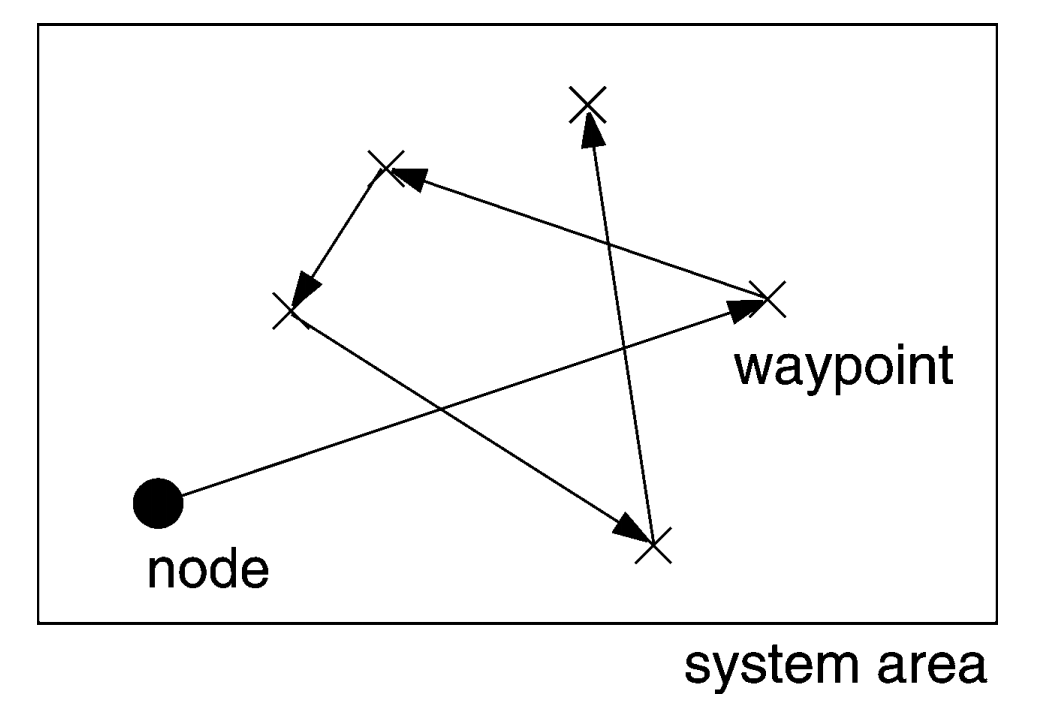
\includegraphics[width=.9\textwidth]{figs/mobilitymodel.PNG}
	\vspace{\baselineskip}
	\caption{Random Waypoint mobility model}
		
	\label{fig:rwpmodel}
\end{figure}


\subsection{Performance Benchmark.}
To evaluate the performance of our algorithm, we compare it to the overall offline optimum that's obtained by solving the optimization formulated in section \ref{section: formulation} using \textit{gurobi}\cite{gurobi}, and the following two edge/cloud-only derivatives of \myalgorithm:
\begin{itemize}
	\item \textbf{Serving on the cloud(SC):} the mobile user would always put the services on the remote cloud to run in order to maximize the computation delay
	\item \textbf{Serving on the edge(SE):} the mobile user would always put the services on the edge servers to run in order to avoid high transmission latency to the cloud. 
\end{itemize}
To show the strength of \myalgorithm\ in terms of scalability, we compare it with the following two greedy learning algorithms:
\begin{itemize}
	\item \textbf{$\epsilon$-greedy.} with a probability of $\epsilon$, randomly choose a super arm, otherwise choose the arm with a maximum average reward
	\item \textbf{Adaptive greedy.} Extension of $\epsilon$-greedy, in which $\epsilon$ is decreasing by time to avoid over-exploring.
\end{itemize}
The parameter used in the simulation is summarized in Table \ref{tab:Simulation parameters}. Nevertheless,  all numeric results are normalized with an appropriate maximum or minimum value from each experiment.


% \begin{figure}
%     \centering
%     \includegraphics[width=0.9\linewidth]{gridsim3.png}
%     \caption{Network topology in simulation}
%     \label{fig:topology simulation}
% \end{figure}
% \subsection{Oracle searching range}
% To explore the optimal oracle search range so that a minimum running time cost is required while the searching area is still wide enough to find the minimal cost, we compare the time cost with service cost within an Oracle at a certain timeslot that has searching range from 1 hop (minimum) to 10 hops (maximum). As shown in figure 7. The optimal service cost can be obtained within minimum two hops while the time cost increases with search range. Therefore setting search range to 2 hops is a optimal solution in our simulation.  

% \begin{figure}
%     \centering
%     \includegraphics[width=0.7\textwidth]{explore.eps}
%     \caption{Exploring Oracle searching range}
%     \label{}
% \end{figure}



% \subsection{\myalgorithm vs. performance benchmark}

% As shown in figure \ref{fig:learningslotbar}, it is easy to find that \myalgorithm algorithm achieves the best performance among other two online algorithms. SE has the worst performance due to the high computation delay on edge.



% \begin{figure}
%     \centering
%     \includegraphics[width=0.9\linewidth]{figs/learningslot1.eps}
%     \caption{The service costs within a certain period}
%     \label{fig:learningslotbar}
% \end{figure}

% \subsection{number of requests}
%\section{Simulation Results}
%In this subsection, we present our simulation results.



\subsection{Impact of network delays}
We considered five levels of computation and transmission delays to investigate their effect on the service quality. 
%We first analyze how the delays (computation delay and transmission delay) in the network setting affect the service performance, and design five levels of computation delay and transmission delay and apply it to the network simulation setting. 
Figure \ref{fig:computingweightbar} and figure \ref{fig:Transmissionweightbar} show that \myalgorithm\ achieves about $15-20\%$ reduction in end-to-end delay compared with other methods. 
For low delays, SE achieves a comparable result because SFCs can be served on the edge with no switching delay due to migration from and to the cloud. SC becomes more competitive when the delays are higher because the computation power of the cloud becomes more significant. Nevertheless, \myalgorithm\ achieves a proper balance between the resources located at the edge and the cloud.



%it is easy to find that \myalgorithm has a overall better performance than the other two derivatives. Specifically, SE has a better performance when either computation and transmission delay is small due to the facts that SFC requests can be served faster on the edge and no switching to the cloud would be involved. However, with the transmission delay or computation delay increasing, it would cost more time to process a SFC request on the edge and thus it has a much worse performance while few performance changes are seen in \myalgorithm and SC.



% \begin{figure}
%     \centering
%     \includegraphics[width=0.9\linewidth]{figs/computationLevel.eps}
%     \caption{Multiple algorithms under different computation settings on edge}
%     \label{fig:computingweightbar}
% \end{figure}

% \begin{figure}
%     \centering
%     \includegraphics[width=0.9\linewidth]{figs/transmissionLevel1.eps}
%     \caption{Multiple algorithms under different transmission settings on edge}
%     \label{fig:Transmissionweightbar}
% \end{figure}

\begin{figure*}[t]
	\centering
	% \begin{subfigure}[b]{.24\textwidth}
	%     \centering
	%     \includegraphics[width=\linewidth]{figs/learningslot2.eps}
	%     \caption{Multiple algorithms under different slots of learning period }
	%     \label{fig:learningslotbar}
	% \end{subfigure}
	\begin{subfigure}[b]{.45\textwidth}
		\centering
		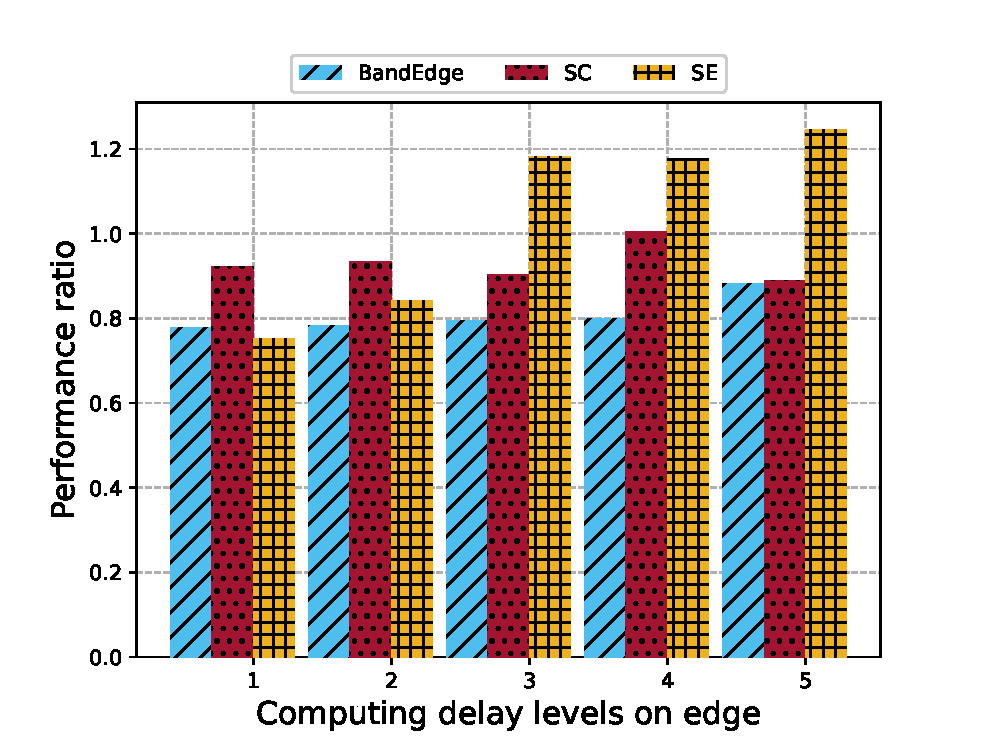
\includegraphics[width=\linewidth]{../icfec21/figs/computationLevel2.eps}
		\caption{Multiple algorithms under different computation settings on edge}
		\label{fig:computingweightbar}
	\end{subfigure}
	\begin{subfigure}[b]{.45\textwidth}
		\centering
		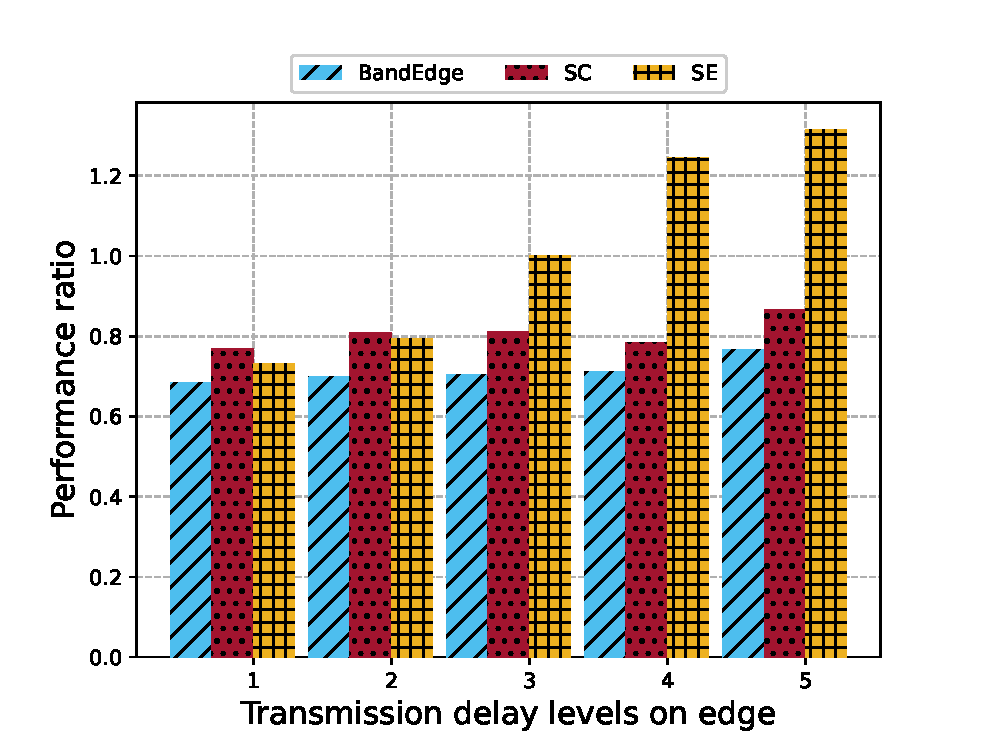
\includegraphics[width=\linewidth]{../icfec21/figs/transmissionLevel2.eps}
		\caption{Multiple algorithms under different transmission settings on edge}
		\label{fig:Transmissionweightbar}
	\end{subfigure}
	% \begin{subfigure}[b]{.45\textwidth}
	%     \centering
	%     \includegraphics[width=\linewidth]{figs/switchingcost2.eps}
	%     \caption{Multiple algorithms under different weights of switching cost}
	%     \label{fig:switchweightbar}
	% \end{subfigure}
		\vspace{\baselineskip}
	\caption{Effect of network delays}
	\label{fig:diff-load}
\end{figure*}


\subsection{Impact of Migration Delay}
Next, we analyze how the switching cost in the network settings affect the service performance. We design five weights of the switching cost to represent the relative importance of migration delay on performance cost while the other setting (\ie, computation and transmission delays) remains the same. As shown in figure \ref{fig:switchweightbar}, the relative performance of all three approaches is similar to that seen in the experiments of delays, which shows that \myalgorithm\ outperform SE and SC in most instances by an overall $20\%$ improvement.
We notice that when the switching weight is high enough (e.g .4.0 or 5.0), \myalgorithm\ has a very similar performance as SC. This is because user prefer to put its services on the same computation node due to high service migration cost and cloud has the most computation capacity.
\begin{figure}
	\centering
	\includegraphics[width=.9\textwidth]{../icfec21/figs/switchingcost2.eps}
		\vspace{\baselineskip}
	\caption{Multiple algorithms under different weights of switching cost}
	\label{fig:switchweightbar}
\end{figure}



Overall, figure \ref{fig:diff-load} and  figure \ref{fig:switchweightbar} shows that \myalgorithm\ is able to jointly consider different types of delay and optimize the
performance with regards to them by jointly utilizing the edge and cloud.

% with the switching cost increasing, the service cost of \myalgorithm become higher compared to SC and SE, particularly, when the weight is at 4.0, the service cost of SC is less than \myalgorithm, this is because SC only put services on the cloud and does not involve service migration at all, while in \myalgorithm and SE, service migration occurs only when the total delay would be dramatically reduced by choosing another computation node or cloud. For example, the service chain demand changes from a light computational service chain task that is served on the edge to a heavy computational service chain task that needs to be migrated to the cloud. Hence the user prefer keep running its service chain on the edge due to a large switching cost to the cloud.



\section{Convergence performance}
\subsection{Comparison with an exact offline approach}
To evaluate the convergence performance of our proposed algorithm, We first trace the average cost of SFC at each timeslot and compare it with a \textit{offline} optimum, which is obtained by solving the exact offline optimization constructed in formulation \ref{formulation:offline}.  Specifically, the offline optimum is calculated after each run of the online algorithm given the whole problem data from the beginning to the end of the learning slots, such as user's demand, mobility, and network capacity on the edge cloud of each online learning experiment.

Figure \ref{fig:Convergence performance} shows that during the learning process, our proposed SFC placement algorithm using \myalgorithm\ gets a decreasing average cost with the time increasing and is gradually converging to a fixed value that is close to the optimum after about 500 time slots. The down-trend indicates that \myalgorithm\ is able to learn the system dynamics and make near-optimal decisions.
% \begin{figure}
%     \centering
%     \includegraphics[width=0.9\linewidth]{figs/replotlearningnormalized.eps}
%     \caption{Time average cost}
%     \label{fig: mainlearningtac}
% \end{figure}

\subsection{Time average regret}
We define the "regret" as the difference between the cumulative estimate cost of the predicted optimal solution at each round calculated using the delay estimates and the actual cost received after playing the predicted solution, denoted by $\hat{c}_t$ and $c_t$ respectively. We can formally define the regret as:
\begin{equation}
	R_T = \sum\limits^T_{t=0} abs(c_t-\hat{c}_t)
\end{equation}
% To analyze the regret, we compare the predicted optimal cost that is calculated using the  delay estimates at each timeslot,  , 
% with an actual cost $c^t_{op}$ obtained by choosing the corresponding optimal estimated arm. The regret is then calculated by $r = \sum^T_{t=0} abs(c^t - c^t_{op})$. In addition, we compare total regret with different values of exploration ration $c$.
From figure \ref{fig:Convergence performance} We can also see a similar trend as the time average cost in total regret during the learning slots, that it increases sharply with learning slots due to the system uncertainty and randomness in the decision making, and gradually converges to a constant value when the time slot is around 2000 times.

\begin{figure}
	\centering
	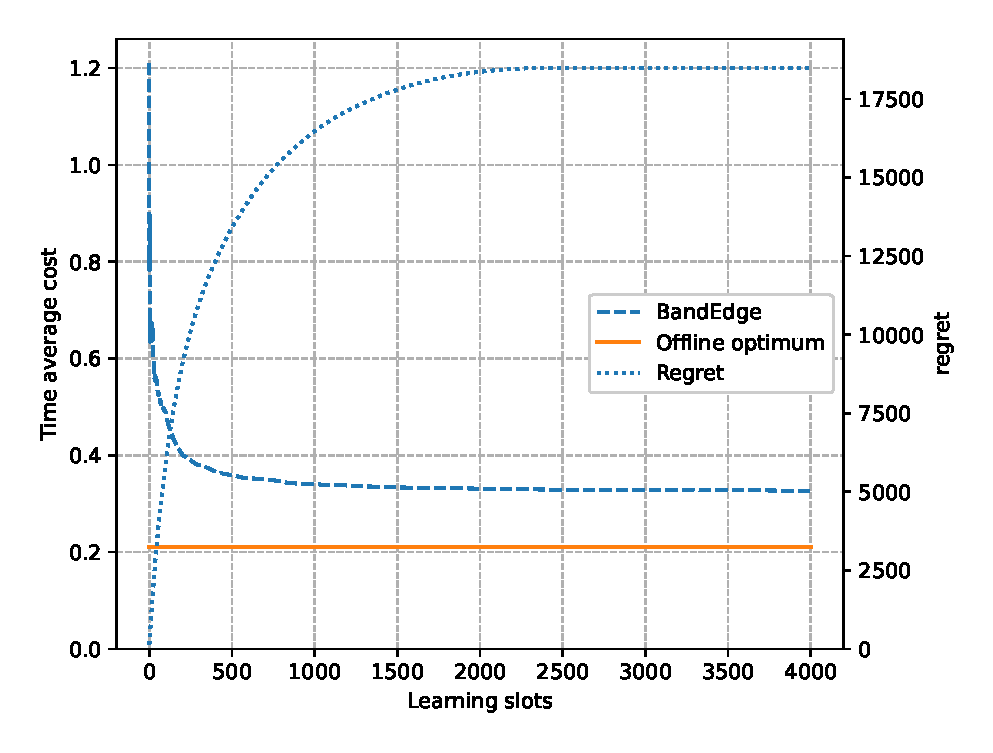
\includegraphics[width=0.9\linewidth]{../icfec21/figs/replotlearningnormalized1.eps}
		\vspace{\baselineskip}
	\caption{Convergence performance: 1) \myalgorithm\ approaching to the offline optimum 2) Algorithm converges around 2000 }
	\label{fig:Convergence performance}
\end{figure}

\subsection{Exploration ratio}
\label{eval:explorationratio}
As mentioned in section\ref{sec:placement algorithm}, exploration level is determined by the ratio $c$ in equation \ref{eqn:delta_hat} when calculating the lower confidence bound for each arm. 
Figure \ref{fig:exploratio} shows how different exploration ratio $c$ influence the total regret of our \myalgorithm\ algorithm. It is observed that a smaller $c$ (e.g, $c = 0.05$) may lead to a lack of exploration, and a bigger $c$ (e.g. $c=1.0$) may lead to over-exploring. We can also see that when $c = 0.3$, the regret converges the fastest. Thus,  it can be used as a fixed value for other experiments. 




\begin{figure}
	\centering
	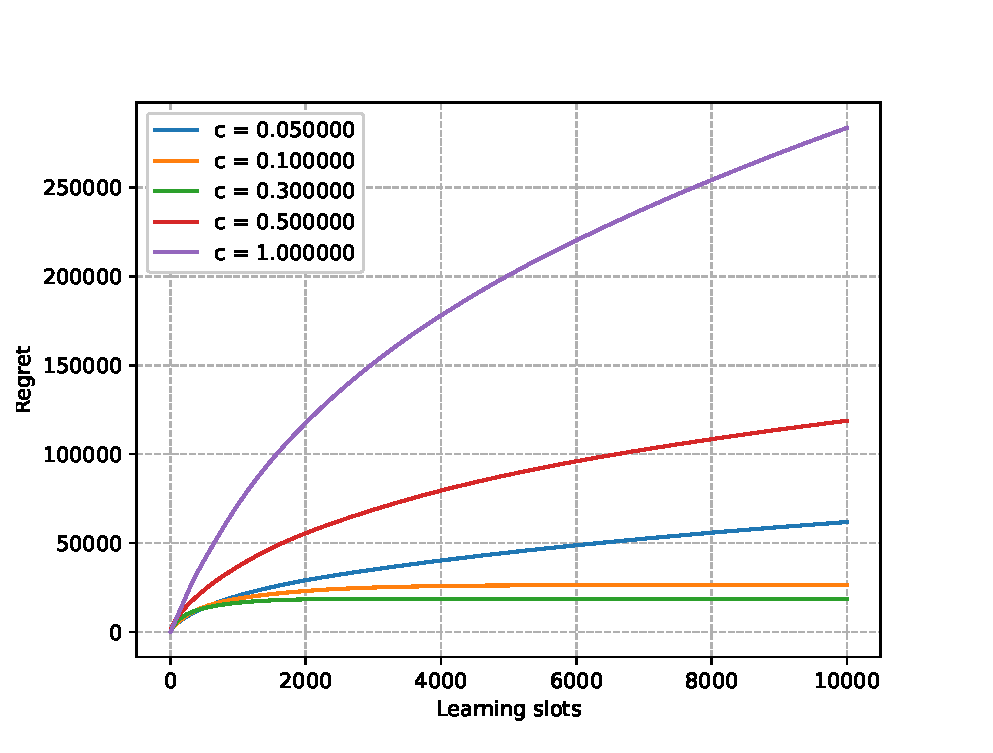
\includegraphics[width=0.9\textwidth]{figs/replotregret1.eps}
		\vspace{\baselineskip}
	\caption{Total regret with different exploration level}
	\label{fig:exploratio}
\end{figure}
% \begin{figure}
%     \centering
%     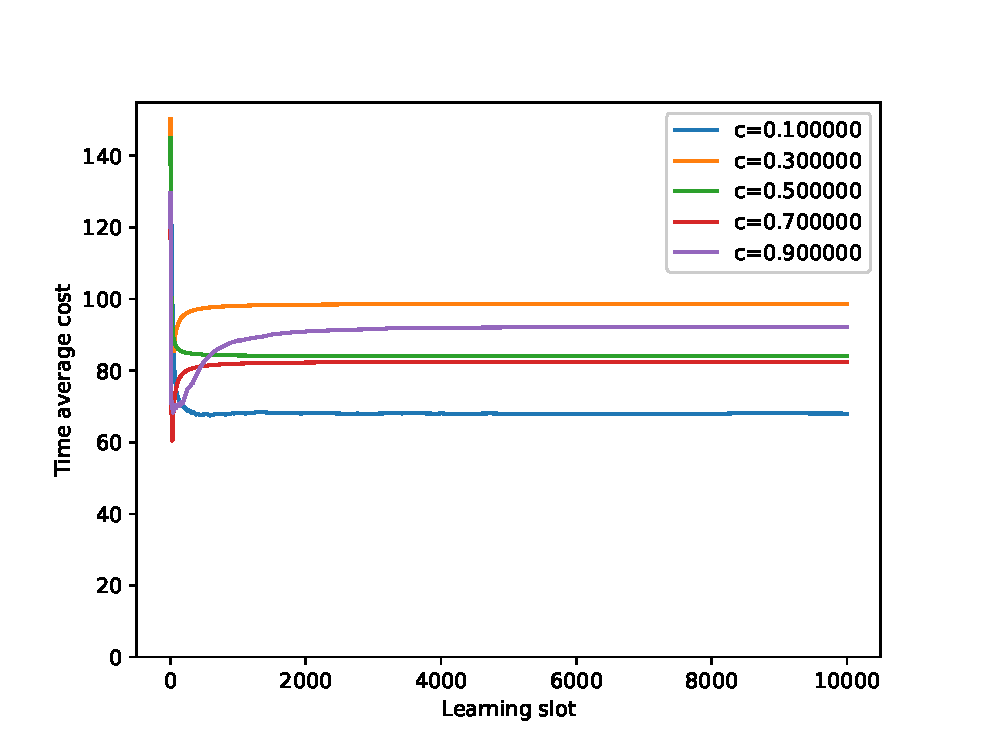
\includegraphics[width=0.9\linewidth]{figs/exploreratio1.eps}
%     \caption{effect of exploration ratio}
%     \label{fig:exploratio}
% \end{figure}

% \begin{figure*}[t]
%     \centering
%     \begin{subfigure}[b]{.45\textwidth}
%         \centering
%         \includegraphics[width=\linewidth]{figs/replotlearningnormalized.eps}
%         \caption{\myalgorithm approaching to the offline optimum}
%         \label{fig: mainlearning}
%     \end{subfigure}
%     \begin{subfigure}[b]{.45\textwidth}
%         \centering
%         \includegraphics[width=\linewidth]{figs/replotsingleregret.eps}
%         \caption{Total regret converges around 2000 learning slots}
%         \label{fig:regret}
%     \end{subfigure}
%     % \begin{subfigure}[b]{.32\textwidth}
%     %     \centering
%     %     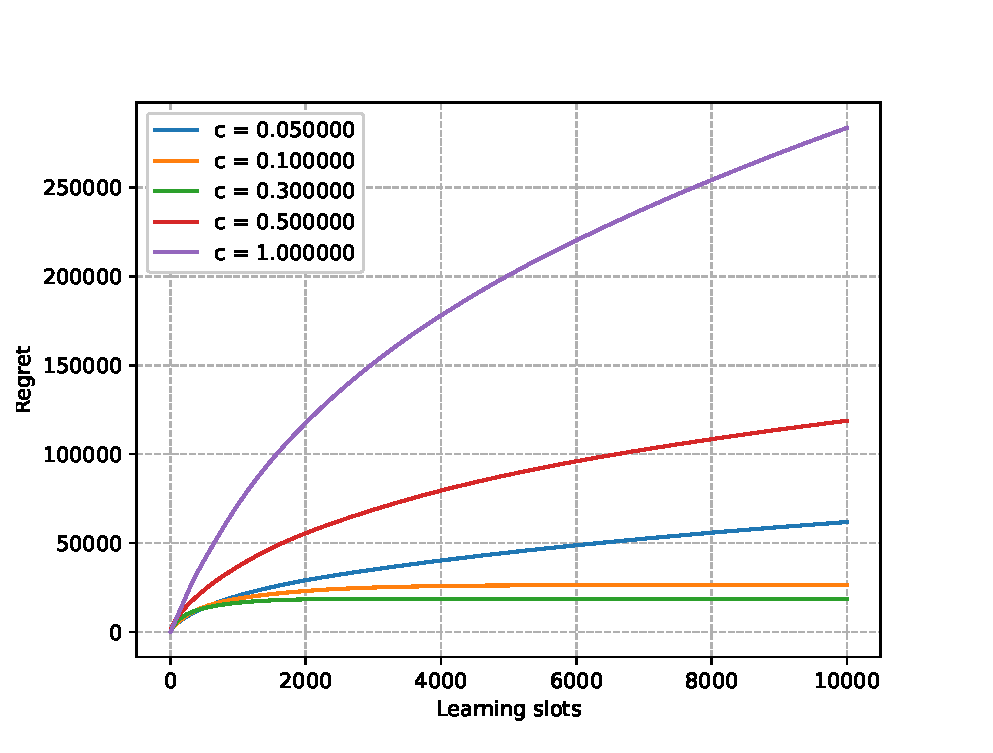
\includegraphics[width=\linewidth]{figs/replotregret1.eps}
%     %     \caption{effect of exploration ratio}
%     %     \label{fig:exploratio}
%     % \end{subfigure}
%     \caption{Convergence performance}
%     \label{fig: Convergence performance}
% \end{figure*}





% \begin{figure}
%     \centering
%     \includegraphics[width=0.9\linewidth]{figs/replotregret.eps}
%     \caption{Regret analysis}
%     \label{fig:regretanalysis}
% \end{figure}
\subsection{Scalability Analysis}
In this section we analyze how \myalgorithm\ is affected by the scale of the problem and compare its performance with the two aforementioned greedy online approaches.

\subsection{Running Time Analysis}
In this experiment, we gradually increased the problem size and computed the running time and cost. 

We increase the network size from 3x3 to 6x6 nodes and specify the number of services on SFC from 3 to 10, then run \myalgorithm\ for 1000 learning slots and calculate the running time. The results are shown in figure \ref{fig:runtimeanalysis}, as expected from the complexity of algorithm \ref{alg:cccpa}, the running time is dominated by the number of available edge servers. Considering that there are 1000 times in this simulation, the average per-time-slot running time is less than 0.3 seconds, which is acceptable for any practical usages.
\begin{figure}
	\centering
	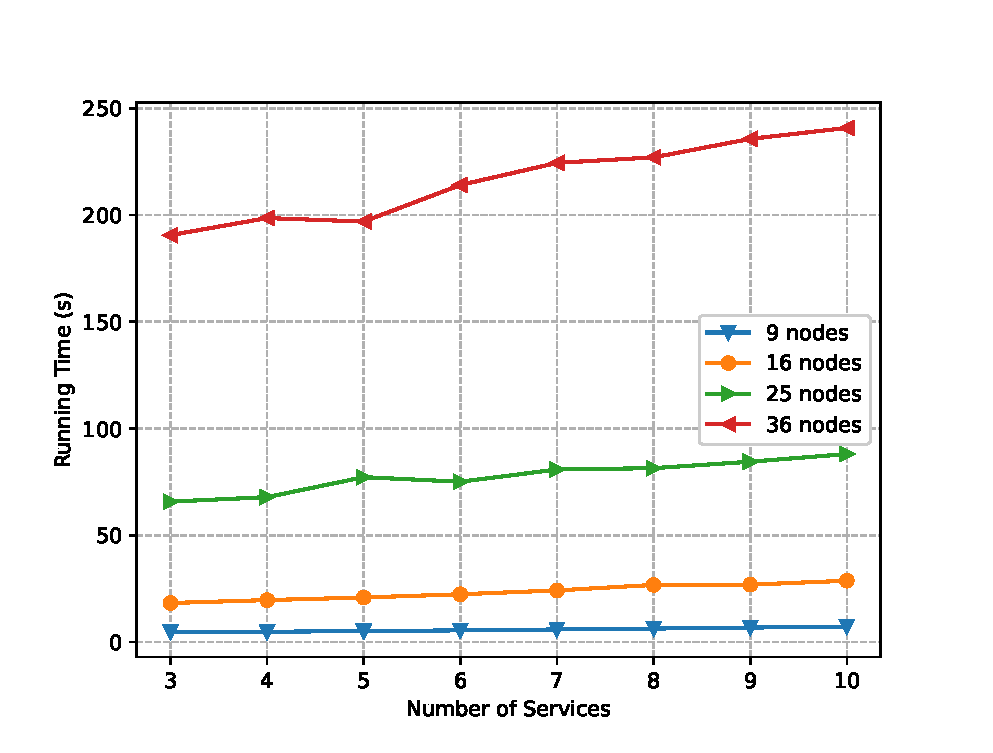
\includegraphics[width=.9\textwidth]{figs/replotruntime_smallfont.eps}
	\vspace{\baselineskip}
	\caption{Run time analysis}
	\label{fig:runtimeanalysis}
\end{figure}





% To analyze how number of services and edge computing nodes influence the algorithm run time, we compute the run time of \myalgorithm with different service number and node number, as shown in figure \ref{fig: runtimeanalysis}, the run time is more influenced by the number of nodes than services, this is due to the time complexity ($O(sn^2)$)of the oracle algorithm.


\subsection{Comparison with the greedy approaches.}
In this experiment, we further compare the cost of \myalgorithm\ with two greedy approaches to show our advantages on performance in terms of problem complexity. As it may be apparent, the difficulty of solving SFC orchestration in our problem depends on the number of services on SFC and the size of the network. Thus, we change these two parameters and see how it affects our algorithm and the greedy algorithms. As shown in figure \ref{fig: scalability}, with the complexity of the problem increases,  the performance of \myalgorithm\ is much less influenced than both greedy algorithms, which shows that our proposed algorithm has better scalability compared to the other two algorithms.
\begin{figure*}[t]
	\centering
	% \begin{subfigure}[b]{.45\textwidth}
	%     \centering
	%     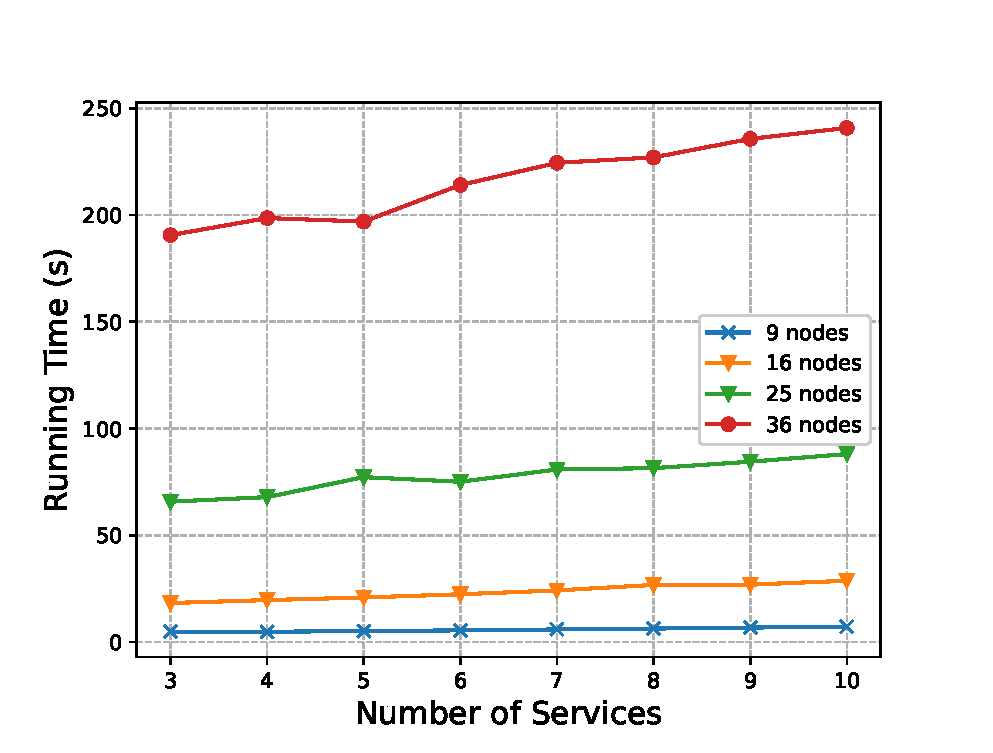
\includegraphics[width=\linewidth]{figs/replotruntime.eps}
	%     \caption{Run time analysis}
	%     \label{fig:runtimeanalysis}
	% \end{subfigure}
	\begin{subfigure}[b]{.45\textwidth}
		\centering
		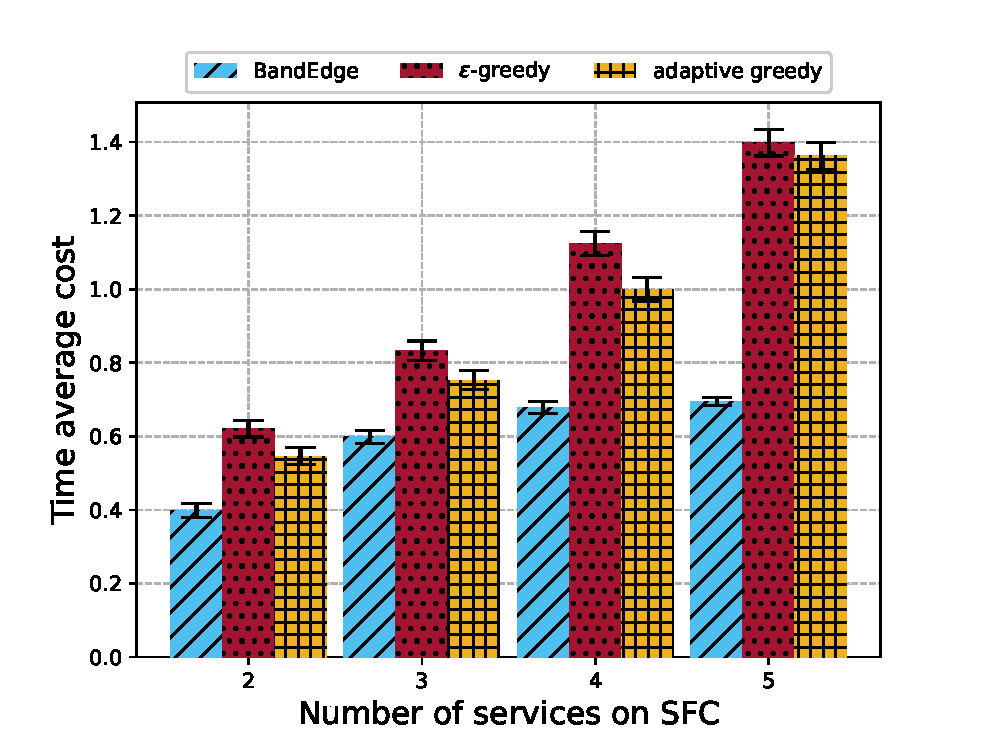
\includegraphics[width=\linewidth]{../icfec21/figs/numservicebar.eps}
		\caption{Number of services on SFC}
		\label{fig:numservicebar}
	\end{subfigure}
	\begin{subfigure}[b]{.45\textwidth}
		\centering
		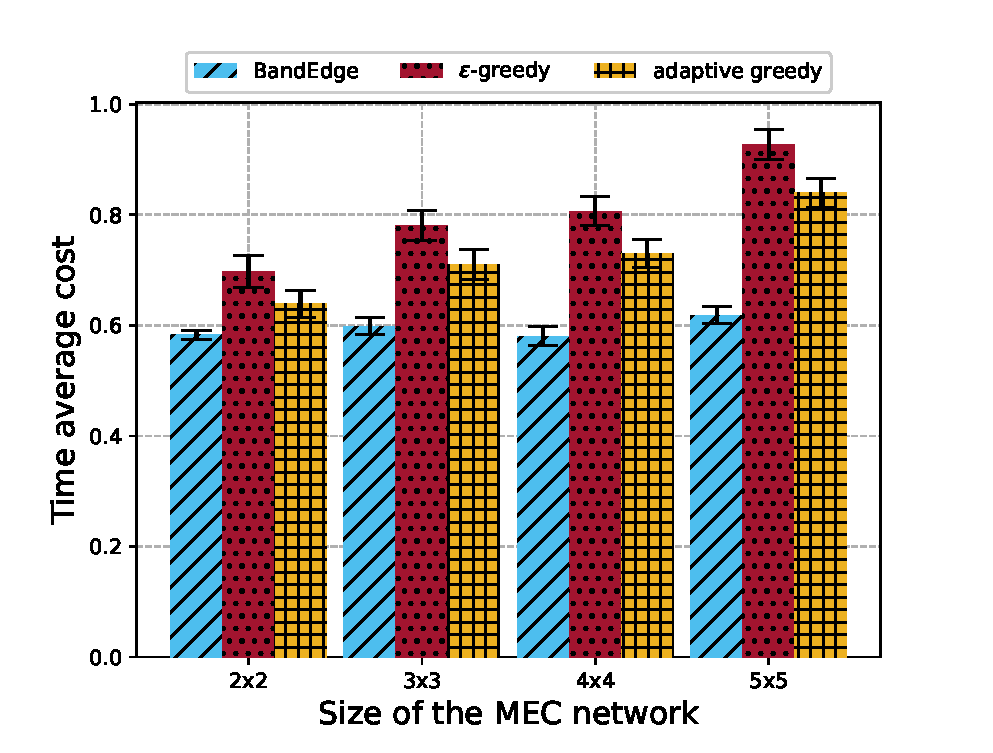
\includegraphics[width=\linewidth]{../icfec21/figs/numnodebar.eps}
		\caption{Size of the MEC network}
		\label{fig:numnodebar}
	\end{subfigure}
	\vspace{\baselineskip}
	\caption{ Performance analysis under different problem scales: a) Number of services on SFC; b) Size of the MEC network}
	\label{fig: scalability}
\end{figure*}





% \begin{figure}
%     \centering
%     \includegraphics[width=0.9\linewidth]{figs/switchingcost.eps}
%     \caption{Multiple algorithms under different weights of switching cost}
%     \label{fig:switchweightbar}
% \end{figure}



% \section{Virtual cluster model}
% Future work discussion
% To simplify the network topology and reduce the number of link arms, we apply $Unison$\cite{vswitch} to convert the grid network topology to a virtual switch cluster topology that is shown in figure 9. All computing nodes including cloud will be connected via a vSwitch.

% \subsubsection{Estimation of the vSwitch and links}


% \begin{figure}
%     \centering
%     \includegraphics[width=0.7\textwidth]{virtualswitch2.png}
%     \caption{Virtual switch cluster}
%     \label{fig:my_label}
% \end{figure}
% \section{Alternative Approaches}
% Besides MAB, we can also apply Reinforcement learning in our model.








\chapter{\textbf{Mininet-WiFi Experiments}}
\label{chapter: Mininet-wifi Experiments}
This chapter describes the Mininet-WiFi experiment we conducted to validate the performance of our proposed user-manged edge-enabled SFC placement in practice. The MEC emulation is implemented as an extension to Mininet-WiFi\cite{mininetwifi}, Mininet-WiFi is a tool that allows researchers to emulate a wireless network environment using SDN technologies. It has supports for the wireless station, Access points, and mobility model. We started by describing the simulation setup and parameters in section \ref{sec:mininetwifisetup}. Then we present the results from the experiments we did in Mininet-WiFi including the learning behavior of \myalgorithm\ in Mininet-WiFi (section \ref{sec:mininetwifilearningbehavior}) and comparison with greedy algorithms under different environmental parameters (section \ref{sec:mobility model experiments}, \ref{sec:mininetwifinetworkdelays}, \ref{sec:mininetwifiSFClength}). 

% In this chapter, we conduct a series of Mininet-WiFi experiments to emulate the MEC wireless network and validate the performance of our SFC placement framework in practice. The MEC emulation is implemented as an extension to Mininet-WiFi\cite{mininetwifi}. Mininet-WiFi is a tool that allow researchers to emulate a wireless network environment using SDN technologies, it has supports for wireless station, Access points and mobility model etc. 



\section{Experiment setup.}
\label{sec:mininetwifisetup}
In our Mininet-WiFi emulation, we create an edge-enabled network with nine wireless base stations that are scattered in a $100\times100$ squared meter area, as shown in figure~\ref{fig:mininettopology}. Each base station is connected to a server that provides computation services. The user, who is connected to the closet base station automatically,  moves with a constant speed that is selected randomly from the interval [1, 5] meters per second. We use the log-distance propagation loss model for wireless connections. We use sockets that run on the edge servers to emulate the computation delay. The user repeatedly sends packets to the closest base station, where the packet is then forwarded to traverse the services in the chain. The last service in the chain sends a response back that allows the user service in the chain sends a response back that allows the user to collect the end-to-end delay (by time-stamping the packets).
The Mininet-WiFi environment is set up in a VM running Ubuntu 16.04.2 LTS with 2 cpu and 4GB RAM. The VM is deployed on a windows 10 machine with i5-7400 and 8GB of RAM.


%we simulate a MEC network that consist of 9 hosts, each of which are attached with an Access Point (AP) that can communicate with mobile user via WiFi and all host are connected using wired Ethernet connections. We then add a moving node as mobile user using a selected mobility model (with a maximum speed of 5 meters/second and minimum speed of 1 meter/s) and propagation model (The Log-Distance Propagation Model) that calculate the power of signal received by the mobile user.
%as show in figure \ref{fig:mininettopology}, the computing nodes are scattered in a 100x100m area with wireless signal range covered the entire area. The Mininet-WiFi environment is set up in a VM running Ubuntu 16.04.2 LTS with 2 cpu and 4GB RAM, which is hosted by a windows 10 machine (i5-7400 \& 8GB RAM).
\begin{figure}
	\centering
	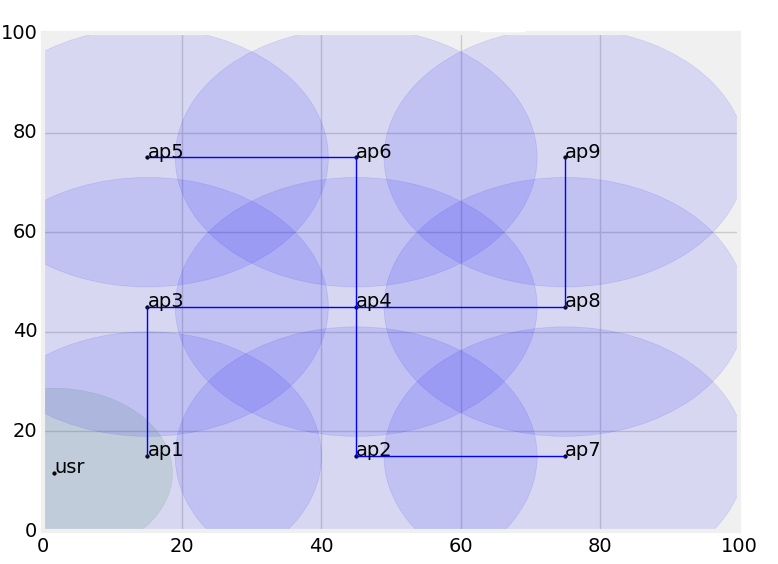
\includegraphics[width=0.9\linewidth]{figs/mininetwifigraph.png}
	\vspace{\baselineskip}
	\caption{Mininet-WiFi Emulation}
	\label{fig:mininettopology}
\end{figure}
%On each edge node, we install server functions that listen for user's request and are configured with different values of computing latency. On user node, we install a client function that sends requests periodically to the servers with dynamic demands and listens for the response.

The parameters used in Mininet-WiFi simulation are summarized as follow:
\begin{itemize}
	\item \textbf{Duration} \textemdash Each experiments ran for 30-60 minutes 
	\item \textbf{Area} \textemdash the spatial area has a dimension $100 \times 100$ meters
	\item \textbf{Mobile stations} \textemdash there is one mobile station representing the mobile user with a mobility model
	\item \textbf{Packet generation rate} \textemdash 25-100 packets per time slot.
	\item \textbf{Packet size} \textemdash fixed to 1 byte.
	\item \textbf{Access Points} \textemdash 9 APs with fixed positions show in figure \ref{fig:mininettopology} with a connection range of 20 meters, which makes 99 \% of the simulation area covered by WiFi, with each of them connected to an edge server.
	\item \textbf{Mobility model} \textemdash five different mobility models analyzed in section \ref{sec:mobility model experiments}, with each configured with a maxmum speed of 5 meters/second and minimum speed of 1 meters/second.
	\item \textbf{Handover policies} \textemdash Active handover, a client station switches WiFi connections to an AP as soon as it finds another connection with closer range, this means that the client is always connected to the closet AP, which is the same as Networx simulation.
	\item \textbf{Propagation model} \textemdash The Log-Distance Propagation Model.
\end{itemize}
%The specifics of The Log-Distance Propagation Model are described as follow:
%
%
%Channel gain, $H$, is calculated by the path-loss with random shadowing,
%\begin{gather}
%    20\times \log{\{\text{distance}^{km}\}} + 28 + \mathcal{N}(0, 5^2), \\
%    H(t)=\frac{10^{-2.8}}{\text{distance}^{2}\times 10^{\mathcal{N}(0, 5^2)/10}}, \\
%    P=10^{1.5}mW.
%\end{gather}
%
%
%Power            = 15 dBm 
%noise            = normal(0,25)
%
%
%P  = 31.6 mW
%H  = 0.01
%Ii = 0.02 mW
%Im = 0.01 mW
%N  = N(0, 25) / 1000 mW
%
%Expect: 
%SNR (signal-to-noise ratio) = (HP)/(Ii+Im+N) = 10
%SNR = 0.316 / (0.03 + N)
%
%Allocated Bandwidth = 1Mhz
%
%Final Bandwidth = 3 Mbps


% \subsection{User machine settings}
% The user machine function as both the SFC request sender and the traffic generator. Specifically,
% the user first send the SFC placement request specifying the SFC placement and the last SFC placement, then a http request that includes all the contextual information above will be generated and sent to the first server on the SFC placement.
% Upon receiving the correct response, the user then start generating traffic and send it to the SFC. It then start listening for a response

% \subsection{Server settings}
% % In our experiment, we implement three VNFs includes an encoder, a decoder and a traffic monitor, which are implemented in Python.
% Accordingly,  the server is also consist of two parts: 
% \begin{enumerate}
%     \item A http server that receives and forwards the SFC placement request, it will also send a VNF migration request to its corresponding server in the last SFC placement; 
%     \item  After the migration and placement is done, the server then start a TCP server that listens for the traffic generated from user, when receiving the traffic, it process each packet with respect to a certain processing delay.
% \end{enumerate}
%  During a SFC placement, the user first sends a SFC placement & migration request, each server that received the request will start listening for traffic while forward the placement request to the next server, when the last server finish placement, it sends a response to user so the user can start sending traffic to the SFC.
%  An example of how the SFC is placed is shown in Figure \ref{fig:SFCplacementdiagramEmulation}, Particularly in Mininet-WiFi emulation, each access point function as both a wireless base station for user and a switch for edge server. 
% \begin{figure}
%     \centering
%     \includegraphics[width=0.9\linewidth]{figs/SFCtrafficmec.PNG}
%     \caption{A placemnent of a simple SFC in MEC}
%     \label{fig:SFCplacementdiagramEmulation}
% \end{figure}

% a TCP server that receives and forwards the traffic
% implemented by python Flask\cite{flask}. Specifically, when running the server, the operator can specify a processing delay, each server will the wait for a SFC request, upon receiving a request, each server will analyze the packet and extract the contextual information such as placement array, last placement array and demand, it first sends a switching request to corresponding server that runs the services in the last timeslot, it the delay the packet for the processing time specified and forward the request to the next placed node according to the placement array. 

% When the last server on the placement array finish its processing, it will return a packet to client.  Upon receiving the return packet, the client will stop recording the time and calculating a end-to-end delay.

% server code will be run on the server hosts

% \subsection{Estimation}
% % Besides SFC request, client can also send a estimation request to a specific computing node, when estimated node receive the request, it will evaluate its processing delay and return it to the client. Client will then calculate the link delay based on the RTT of each estimation packet.

% \subsection{Time stamp based delay estimation}
% To estimate the delays in the network, we simply time-stamp the packets we send and keep track of the time. The estimation are consist of two parts:
% \begin{enumerate}
%     \item An initial estimation of the whole network. The user first sends a request to each computing node, upon receiving the request, the server will each send packets to the other servers and time stamp them. After receiving all the returned packets, the server parse the time stamps in them, calculate the delays and send those information back to the user. The user collect all the delay estimations from the servers and save it as a initial estimation that is required in the \myalgorithm algorithm
%     \item An estimation of delays on the SFCs we have tried. Like the initial estimation, we also time stamp the packets we send in each SFC request, after the packet is returned from the SFC, the user parse the time stamps and calculate the delays on the SFC. Those estimation will then be used to update the initial estimation according to algorithm 1.
% \end{enumerate}
% Due to the noise delay (e.g. time consumed other than transmission and processing) in the network, the estimated processing delay may be higher than the actual delay,  that is 

% \begin{equation}
%     \mu = (\lambda * c_i + n)/\lambda
% \end{equation}

% However, when we estimate the overall processing time, there might be some error depends on the demand $\lambda$, that is:
% \begin{equation}
%     t_{proc} = \mu * \lambda' = (\lambda * c_i + n)/\lambda *\lambda'
% \end{equation}


\section{\myalgorithm\ performance in Mininet-WiFi.}
\label{sec:mininetwifilearningbehavior}
In this experiment, we perform the actual placement of the SFCs on an emulated Mininet-WiFi network topology, as shown in figure 16. Specifically, we first run the time-stamp estimation on the whole network and gain an initial estimation. Based on the initial estimation, we apply \myalgorithm\ to calculate an optimal SFC and perform the placement. When the SFC servers are ready to listen for the traffic, we then assign a corresponding amount of packets to each server on SFC according to the SFC request, forward them through the SFC and record their end-to-end delay s (\textit{i.e.}, by time-stamping the data packets). We keep the trace of the average response time of each request in this experiment and compare the result to the aforementioned offline optimum and $\epsilon$-greedy algorithm. 

The network settings we use in our experiment are shown in table \ref{tab:network settings}. More specifically, each service request on the SFC is randomly chosen from [10, 25, 100] bytes (e.g. for a SFC with three services: [25, 10, 100] bytes). In our emulation, each packet contains one byte of data (e.g. 100 packets will be sent in a SFC request of 100 bytes), we configure the computing delays to be the time it takes for a server to process one packet, which varies from 10 to 50 ms/bytes, and the switch delays to be proportional to link delays, which vary from the range of [100, 500]ms and [400, 2000]ms, respectively.

\begin{table}
	\centering
	\setcellgapes{5pt}
	\caption{Network and VNF setting}
	\label{tab:network settings}
	% \resizebox{\columnwidth}{!}
	\begin{tabular}{ll}
		
		\toprule
		Parameter & Value \\ [5pt]
		\midrule
		VNFs per SFC  &  2-4\\[5pt]
		VNF request (byte) & [10, 25, 100]\\[5pt]
		Link delay (ms)  & 100 - 500 \\[5pt]
		Migration delay (ms) & 400 - 2000 \\[5pt]
		VNF proc.delay (ms/byte) & 10 - 50 \\[5pt]
		Minimum speed & 1 m/s \\[5pt]
		Maximum speed & 5 m/s \\ [5pt]
		\bottomrule
	\end{tabular}
\end{table}

\subsection{Response Time}
Figure \ref{fig:myalgorithm performance} shows the convergence performance of \myalgorithm\ algorithm in an emulated wireless network using the network settings shown in table \ref{tab:network settings}. As anticipated, despite getting unstable averages initially, \myalgorithm\ \ gets a decreasing average cost as the learning slot increases and converges to a stable level, which has similar traits as the convergence performance in simulations. The results also show that \myalgorithm\ outperforms $\epsilon$-greedy over the entire course of 1000 learning slots. This is because $\epsilon$-greedy does not select arms combinatorially, and therefore has more extensive decision space than \myalgorithm, which results in a worse learning performance than \myalgorithm.
\begin{figure}
	\centering
	\includegraphics[width=0.9\linewidth]{../icfec21/figs/MiniwifiLearning1.eps}
	\vspace{\baselineskip}
	\caption{\myalgorithm\ outperform $\epsilon$-greedy in Mininet-WiFi}
	\label{fig:myalgorithm performance}
\end{figure}


% \subsection{effect of service number}
% In this experiment, we compare our estimated response time that is calculated by the estimated network delays using \myalgorithm model with the actual response time we observe from running SFC requests. Specifically, adjustment in equation \ref{eqn:adjustment} will be applied when calculating the estimated response time.
% Figure \ref{fig:EstimationvsEmulation} shows that with the learning slot increasing, average response time in Mininet-WiFi experiment is decreasing, this is expected. The figure also shows that the difference between the estimation and emulation are decreasing and the estimation time is smaller than the emulation. This is because estimation gets more accurate with the learning going further, however, it is still lower than the actual delay because of the noise delay in the network that we did not consider in our model. 



% \noindent\textbf{Practical performance evaluation.}
% In this section we analyze the practical performance of our proposed algorithm and compare it with two greedy algorithms introduced in simulation experiments.

In the next sections, we evaluate the total response time of \myalgorithm\ in Mininet-WiFi under different environmental parameters such as Mobility models, network delay, and length of the SFC, then compare the respnse time with the two aforementioned greedy approaches.

\subsection{User Mobility analysis}
\label{sec:mobility model experiments}
We first investigate how the mobility model affects the end-to-end latency. Specifically, we consider the following mobility models:

\cat{RW} random walk, a variant of the random waypoint model\cite{rwp}, where the user moves directly towards the next waypoint at a certain velocity and choose the next waypoint and velocity randomly. Compared to the random waypoint model, the random walk model has a constant velocity and does not have a wait time.

\cat{RD} random direction, a variant of the random waypoint model, compared to the random waypoint, the only difference is that the user has no wait time. The user travel with a velocity that is uniformly distributed between the minimum velocity and maximum velocity.

\cat{TVC} Time-Variant Community, In this model, the user will periodically re-appear at the same location defined as \say{communities}.

\cat{GM} Gauss Markov, in this model, the velocity of the mobile user is assumed to be correlated over time and modeled as a Gauss-Markov stochastic process.

\cat{RP} Reference Point, this model simulates a group behavior where the user follows a group leader and are randomly distributed around a reference point. The user has a velocity and direction randomly derived from that of the group leader.

\begin{figure}
	\centering
	\includegraphics[width=0.9\linewidth]{../icfec21/figs/mobilitymodel2.eps}
	\vspace{\baselineskip}
	\caption{Effect of mobility models}
	\label{fig:Mobility models}
\end{figure}

Figure \ref{fig:Mobility models} shows the performance of \myalgorithm\ under different mobility models in Mininet-WiFi, from which we can see that different mobility model can result in various average response time for both greedy and \myalgorithm\ algorithms, this is due to multiple parameters in a mobility model such as average velocity, wait time and mobility range. For example, the RD model results in a higher response time than RW because the user's velocity is continuously changing in RD while the RW model sets the user in a constant velocity.

\subsection{Different network delays}
\label{sec:mininetwifinetworkdelays}
In this experiment, we analyze the impact of different delay settings (e.g. per-packet computing delay and transmission delay) on the average response time after 500 timeslots. The response time increase as the link delay increases. The results are shown in figure \ref{fig:link delay bar} and figure \ref{fig:processing delay bar} ,respectively. It can also be observed that the processing delay has a greater impact on the overall response time than transmission delay in Mininet-WiFi emulation, which is often the case in most real-world SFC applications.
\begin{figure*}[t]
	\centering
	\begin{subfigure}[b]{.45\textwidth}
		\centering
		\includegraphics[width=\linewidth]{../icfec21/figs/linkdelaybar.eps}
		
		\caption{Effect of link delay}
		\label{fig:link delay bar}
	\end{subfigure}
	\begin{subfigure}[b]{.45\textwidth}
		\centering
		\includegraphics[width=\linewidth]{../icfec21/figs/prodelaybar.eps}
		
		\caption{Effect of processing delay}
		\label{fig:processing delay bar}
	\end{subfigure}
	% \begin{subfigure}[b]{.45\textwidth}
	%     \centering
	%     \includegraphics[width=\linewidth]{figs/mobilitymodel2.eps}
	%     \caption{Effect of mobility models}
	%     \label{fig:Mobility models}
	% \end{subfigure}
	% \begin{subfigure}[b]{.45\textwidth}
	%     \centering
	%     \includegraphics[width=\linewidth]{figs/numservicebarmininet.eps}
	%     \caption{Effect of the length of SFC}
	%     \label{fig:num service mininet bar}
	% \end{subfigure}
		\vspace{\baselineskip}
	\caption{Effect of Mininet-WiFi network delays: a) link delay; b) processing delay}
	\label{fig:environparameter-mininet}
\end{figure*}
\subsection{Different length of SFC.}
\label{sec:mininetwifiSFClength}
Figure \ref{fig:num service mininet bar} shows the effect of SFC length (e.g the number of VNFs on each SFC) on average response time. As expected, response times increases as the length of SFC increases. 
\begin{figure}
	\centering
	\includegraphics[width=.9\textwidth]{../icfec21/figs/numservicebarmininet.eps}
	\vspace{\baselineskip}
	\caption{Effect of the length of SFC}
	\label{fig:num service mininet bar}
\end{figure}

Overall, figure \ref{fig:environparameter-mininet} and \ref{fig:num service mininet bar} shows that \myalgorithm outruns the two greedy approaches by about 1 to 5 seconds under varying environmental settings.

% \begin{figure}
%     \centering
%     \includegraphics[width=0.9\linewidth]{figs/linkdelaybar.eps}
%     \caption{effect of link delay}
%     \label{fig:link delay bar}
% \end{figure}

% \begin{figure}
%     \centering
%     \includegraphics[width=0.9\linewidth]{figs/prodelaybar.eps}
%     \caption{effect of processing delay}
%     \label{fig:processing delay bar}
% \end{figure}



% \begin{figure}
%     \centering
%     \includegraphics[width=0.9\linewidth]{figs/replot6.eps}
%     \caption{effect of exploration ratio}
%     \label{fig:explorationc}
% \end{figure}
\chapter{\textbf{Conclusion}}

Mobile Edge Computing (MEC) empowers cloud computing by distributing cloud resources (\eg storage and processing capacity) to the edge servers inside the range of radio access network (RAN) and bring them closer to end-users. It provides end-users with swift and powerful computing, energy efficiency, storage capacity, mobility, location, and context awareness support. Network Function Virtualization (NFV) enables scalable resource allocation, agile deployment, and efficient management of network services. It largely reduces the deploying and managing cost. 
Applying NFV to MEC will not only reduce the overall latency for end-users but also provide them with lower cost and flexible management over network services. One of the main considerations when applying NFV to MEC is the placement of Service Function Chains (SFC) on edge, where more changes such as service migration and user mobility need to be addressed. 

%Many existing works in the literature have discussed SFC placement, these works, however, either mainly focus on $system-managed$ SFC placement that system-wide information is known or lack consideration of MEC contexts such as users mobility and service migration. 

In this work, we addressed the problem of user-managed service function chain orchestration with the objective of end-to-end delay optimization in mobile edge computing while considering
the service migration cost and user mobility. We formulated
the problem as an integer linear program and used its solution as an offline performance benchmark.
In order to handle the uncertainties in the real environment, we applied the theory of contextual bandits, which reduces the problem complexity and utilizes the available information to make efficient decisions.
Then, we used an efficient dynamic programming method to perform the chain orchestration task, which computes delay-optimized SFC placements in polynomial time.
At last, through extensive simulations and emulations, we analyzed the utility and performance of our algorithm.

Section \ref{section: thesis summary} of this chapter summarize the thesis with regards to our research focus and Section \ref{section:future work} discuss the future research directions.



\section{Thesis Summary}
\label{section: thesis summary}
In Chapter 1, we discussed the concept of NFV and MEC, as well as the advantages and challenges when applying NFV to MEC. There are three challenges in user-managed SFC placement on edge: Unknown system-wide information such as dynamic network capacities, user's mobility within MEC, and VNF migrations due to the user's mobility.  We also briefly introduced the approaches taken to address the aforementioned challenges and the main contributions of this work.

Chapter 2 provided readers with the background information for acknowledging the work in this thesis. Particularly, we provided a summary of basic knowledge on NFV, SFC, and MEC architecture, then, we introduced the online learning techniques concerned in this work, including Greedy Multi-Arm Bandit learning and Combinatorial Contextual Multi-arm Bandit learning, and the mathematical techniques applied in this work including Binary Integer Linear Program, Binary Product Linearization and Dynamic Programming. We also summarized the software tools used in simulation and emulation, including Networkx simulator, Gurobi Optimizer, and Mininet-WiFi emulator.

In Chapter 3, we review and categorize the previous works that solve the SFC placement into four classes based on their problem model: system-managed edge-agnostic, system-managed edge-enabled, user-managed edge-agnostic, and user-managed edge-enabled. For each work reviewed, we discuss their system model, objective, and the applied optimization approaches and algorithms, as well as their weakness and relevance to our work.

Chapter 4 describes the mathematical models we adopt in this work in order to modelize the SFC placement in the mobile edge computing system,  including network model and demand model, then we formally defined the user-managed edge-enabled SFC placement as a contrained optimization problem with the objective of minimizing the total end-to-end delay, which is formulated as a Binary Integer Linear Program problem. 

In chapter 5, we present our proposed contextual combinatorial bandit formulation for the user-managed edge-enabled SFC placement problem. Specifically, we first utilize an unknown parameter vector for each server and link to capture and learn the system-wide information, including processing and bandwidth capacities. We then associate each server and link with a feature vector that characterizes user's side contextual information such as their service demand, current location, and previous SFC placement.  Then, we define a linear reward function that utilizes the two aforementioned vectors to calculate the delays on each arm (\ie\ each server and link). We further prove that with the proposed combinatorial bandit formulation, the decision space of the user can be considerably reduced compared to a general multi-arm bandit formulation.
Finally, we present our proposed bandit-based algorithm \myalgorithm, that adopts the \textit{upper confidence bound} theory to maintain confidence bound for each arm during the learning slots and uses dynamic programming algorithm to compute the optimal placement solution in polynomial time at every single time slot.

Chapter 6 provides a brief idea and design of the delay estimation framework that is required in the bandit formulation. The main idea of this framework is to use timestamps to record and keep track of the delays experienced on each node and link when network packets are routed through SFCs.

Chapter 7 presents extensive simulation results that demonstrate the performance of our proposed algorithm. The results show that \myalgorithm\ can cope with the system uncertainty and make balanced decisions in terms of migration, exploration, and exploitation under different system dynamics. 
We then study the learning behavior and convergence performance by analyzing the time average cost and total regrets during the learning slots and compare it with an optimal offline benchmark.
We further studied the performance of our proposed algorithm against greedy approaches under different problem sizes. The comparison results show that our proposed algorithm outperforms the greedy approaches by at least 50 percent in terms of scalability.

Chapter 8 reported the results of realistic Mininet-wifi experiments we conduct in order to validate the superior performances of our proposed algorithm under the emulated wireless network environment.
The collected empirical data indicate that our proposed algorithm has a similar learning behavior as simulation.
We further study the performance of \myalgorithm\ under different network delay settings,  mobility models, and SFC lengths. The result of this experiment shows that the performance observed in simulation is indeed achievable in practice.




% In this thesis, we study the SFC placement problem in a NFV-enabled MEC. We focus on a user-managed SFC placement problem and seek to optimize the end-to-end delay while taken migration, user's mobility and user specific demands taken into consideration. For which we proposed an exact offline problem formulation and an online learning approaches that is based on multi-arm bandit theory. 
% In order to characterize the attribute on each computing node and link, we formulate the placement problem as a contextual combinatorial MAB problem and balancingly explore and exploit the value on each feature by updating its upper confidence bound at each round. Furthermore, we designed a dynamic program based SFC allocation approach that is able to find per-time-slot optimum in a polynomial time and integrate it the learning frame. Lastly, through extensive simulations and emulations, we are able to demonstrate the superior performance of our algorithm.


\section{Future work}
\label{section:future work}

\cat{SFC placement Strategies}
We resort to using a dynamic programming approach to compute the placement solution at every single time slot. While we can attain the exact optimum using this approach, developing approximate placement algorithms that achieve near-optimum performance can result in less run time cost when the problem size is very large.



\cat{Network Topologies}
The edge computing network topology we used in our simulation and emulation experiments were designed to be squared grid structures. An interesting research direction would be to consider other types of network topologies (\eg, cluster topology) in the experiments. 


\cat{Cooperation in Practice}
In this work, we analyze the performance of \myalgorithm\ on both model-driven simulation and realistic Mini-WiFi emulations. A valuable next step is to implement and deploy such algorithm in a real-world MEC network for more empirical analysis.




\appendix
%%\fancyhead[RO,LE]{\thepage}
%\fancyfoot{}

\chapter{First Appendix}

%Start the body text
Lorem ipson dolor sic amet sec in consetum epsom nunc ad valorem. Lorem ipson dolor sic amet
sec in consetum nunc ad valorem. Lorem epsom ipson dolor sic amet sec in consetum nunc ad valorem.
Lorem ipson dolor sic amet sec in consetum nunc ad valorem. Lorem ipson dolor sic amet
sec in consetum nunc ad valorem. Lorem ipson dolor sic amet sec in epsom consetum nunc ad valorem.

Lorem ipson dolor sic amet sec in consetum epsom nunc ad valorem. Lorem ipson dolor sic amet
sec in consetum nunc ad valorem. Lorem epsom ipson dolor sic amet sec in consetum nunc ad valorem.
Lorem ipson dolor sic amet sec in consetum nunc ad valorem. Lorem ipson dolor sic amet
sec in consetum nunc ad valorem. Lorem ipson dolor sic amet sec in epsom consetum nunc ad valorem.
Lorem ipson dolor sic amet sec in consetum epsom nunc ad valorem. Lorem ipson dolor sic amet
sec in consetum nunc ad valorem. Lorem epsom ipson dolor sic amet sec in consetum nunc ad valorem.
Lorem ipson dolor sic amet sec in consetum nunc ad valorem. Lorem ipson dolor sic amet
sec in consetum nunc ad valorem. Lorem ipson dolor sic amet sec in epsom consetum nunc ad valorem.
Lorem ipson dolor sic amet sec in consetum epsom nunc ad valorem. Lorem ipson dolor sic amet
sec in consetum nunc ad valorem. Lorem epsom ipson dolor sic amet sec in consetum nunc ad valorem.
Lorem ipson dolor sic amet sec in consetum nunc ad valorem. Lorem ipson dolor sic amet
sec in consetum nunc ad valorem. Lorem ipson dolor sic amet sec in epsom consetum nunc ad valorem.

Lorem ipson dolor sic amet sec in consetum epsom nunc ad valorem. Lorem ipson dolor sic amet
sec in consetum nunc ad valorem. Lorem epsom ipson dolor sic amet sec in consetum nunc ad valorem.
Lorem ipson dolor sic amet sec in consetum nunc ad valorem. Lorem ipson dolor sic amet
sec in consetum nunc ad valorem. Lorem ipson dolor sic amet sec in epsom consetum nunc ad valorem.
Lorem ipson dolor sic amet sec in consetum epsom nunc ad valorem. Lorem ipson dolor sic amet
sec in consetum nunc ad valorem. Lorem epsom ipson dolor sic amet sec in consetum nunc ad valorem.
Lorem ipson dolor sic amet sec in consetum nunc ad valorem. Lorem ipson dolor sic amet
sec in consetum nunc ad valorem. Lorem ipson dolor sic amet sec in epsom consetum nunc ad valorem.
\begin{figure}
Place the figure here
\caption{Figure in the appendix}
\end{figure}

Lorem ipson dolor sic amet sec in consetum epsom nunc ad valorem. Lorem ipson dolor sic amet
sec in consetum nunc ad valorem. Lorem epsom ipson dolor sic amet sec in consetum nunc ad valorem.
Lorem ipson dolor sic amet sec in consetum nunc ad valorem. Lorem ipson dolor sic amet
sec in consetum nunc ad valorem. Lorem ipson dolor sic amet sec in epsom consetum nunc ad valorem.
Lorem ipson dolor sic amet sec in consetum epsom nunc ad valorem. Lorem ipson dolor sic amet
sec in consetum nunc ad valorem. Lorem epsom ipson dolor sic amet sec in consetum nunc ad valorem.
Lorem ipson dolor sic amet sec in consetum nunc ad valorem. Lorem ipson dolor sic amet
sec in consetum nunc ad valorem. Lorem ipson dolor sic amet sec in epsom consetum nunc ad valorem.

Lorem ipson dolor sic amet sec in consetum epsom nunc ad valorem. Lorem ipson dolor sic amet
sec in consetum nunc ad valorem. Lorem epsom ipson dolor sic amet sec in consetum nunc ad valorem.
Lorem ipson dolor sic amet sec in consetum nunc ad valorem. Lorem ipson dolor sic amet
sec in consetum nunc ad valorem. Lorem ipson dolor sic amet sec in epsom consetum nunc ad valorem.
Lorem ipson dolor sic amet sec in consetum epsom nunc ad valorem. Lorem ipson dolor sic amet
sec in consetum nunc ad valorem. Lorem epsom ipson dolor sic amet sec in consetum nunc ad valorem.
Lorem ipson dolor sic amet sec in consetum nunc ad valorem. Lorem ipson dolor sic amet
sec in consetum nunc ad valorem. Lorem ipson dolor sic amet sec in epsom consetum nunc ad valorem.

Lorem ipson dolor sic amet sec in consetum epsom nunc ad valorem. Lorem ipson dolor sic amet
sec in consetum nunc ad valorem. Lorem epsom ipson dolor sic amet sec in consetum nunc ad valorem.
Lorem ipson dolor sic amet sec in consetum nunc ad valorem. Lorem ipson dolor sic amet
sec in consetum nunc ad valorem. Lorem ipson dolor sic amet sec in epsom consetum nunc ad valorem.
Lorem ipson dolor sic amet sec in consetum epsom nunc ad valorem. Lorem ipson dolor sic amet
sec in consetum nunc ad valorem. Lorem epsom ipson dolor sic amet sec in consetum nunc ad valorem.
Lorem ipson dolor sic amet sec in consetum nunc ad valorem. Lorem ipson dolor sic amet
sec in consetum nunc ad valorem. Lorem ipson dolor sic amet sec in epsom consetum nunc ad valorem.
\begin{table}
\caption{Table in the appendix}
\center{Place the table here}
\end{table}
Lorem ipson dolor sic amet sec in consetum epsom nunc ad valorem. Lorem ipson dolor sic amet
sec in consetum nunc ad valorem. Lorem epsom ipson dolor sic amet sec in consetum nunc ad valorem.
Lorem ipson dolor sic amet sec in consetum nunc ad valorem. Lorem ipson dolor sic amet
sec in consetum nunc ad valorem. Lorem ipson dolor sic amet sec in epsom consetum nunc ad valorem.
Lorem ipson dolor sic amet sec in consetum epsom nunc ad valorem. Lorem ipson dolor sic amet
sec in consetum nunc ad valorem. Lorem epsom ipson dolor sic amet sec in consetum nunc ad valorem.
Lorem ipson dolor sic amet sec in consetum nunc ad valorem. Lorem ipson dolor sic amet
sec in consetum nunc ad valorem. Lorem ipson dolor sic amet sec in epsom consetum nunc ad valorem.

Lorem ipson dolor sic amet sec in consetum epsom nunc ad valorem. Lorem ipson dolor sic amet
sec in consetum nunc ad valorem. Lorem epsom ipson dolor sic amet sec in consetum nunc ad valorem.
Lorem ipson dolor sic amet sec in consetum nunc ad valorem. Lorem ipson dolor sic amet
sec in consetum nunc ad valorem. Lorem ipson dolor sic amet sec in epsom consetum nunc ad valorem.
Lorem ipson dolor sic amet sec in consetum epsom nunc ad valorem. Lorem ipson dolor sic amet
sec in consetum nunc ad valorem. Lorem epsom ipson dolor sic amet sec in consetum nunc ad valorem.
Lorem ipson dolor sic amet sec in consetum nunc ad valorem. Lorem ipson dolor sic amet
sec in consetum nunc ad valorem. Lorem ipson dolor sic amet sec in epsom consetum nunc ad valorem.


Lorem ipson dolor sic amet sec in consetum epsom nunc ad valorem. Lorem ipson dolor sic amet
sec in consetum nunc ad valorem. Lorem epsom ipson dolor sic amet sec in consetum nunc ad valorem.
Lorem ipson dolor sic amet sec in consetum nunc ad valorem. Lorem ipson dolor sic amet
sec in consetum nunc ad valorem. Lorem ipson dolor sic amet sec in epsom consetum nunc ad valorem.
Lorem ipson dolor sic amet sec in consetum epsom nunc ad valorem. Lorem ipson dolor sic amet
sec in consetum nunc ad valorem. Lorem epsom ipson dolor sic amet sec in consetum nunc ad valorem.
Lorem ipson dolor sic amet sec in consetum nunc ad valorem. Lorem ipson dolor sic amet
sec in consetum nunc ad valorem. Lorem ipson dolor sic amet sec in epsom consetum nunc ad valorem.




\bibliographystyle{plainurl}
\bibliography{ref}
\end{document}
